\section{ÔN TẬP THPTQG 2026 - GÓC - KHOẢNG CÁCH - THỂ TÍCH}
\subsection{Ví dụ}
\begin{vd}%[1H8H5-2]
Cho hình chóp $A.BCD$ có cạnh $AC \perp (BCD)$ và $BCD$ là tam giác đều cạnh bằng $a$. Biết $AC=a\sqrt{2}$ và $M$ là trung điểm của $BD$. Xét tính đúng, sai các khẳng định sau:
\choiceTF[1t]
{$\mathrm{d}(C,BD)=\dfrac{a\sqrt{2}}{2}$}
{Khoảng cách từ $A$ đến $BD$ là $\dfrac{a\sqrt{11}}{3}$}
{\True $\mathrm{d}(B,AD)=\mathrm{d}(D,AB)$}
{\True Khoảng cách từ $C$ đến $AM$ là $a\sqrt{\dfrac{6}{11}}$}
\loigiai
{ \begin{center}
\begin{tikzpicture}[scale=1.0, font=\footnotesize, line join=round, line cap=round, >=stealth]
\draw (0,0) node[left]{$C$}circle (1pt);
\draw (2,-2) node[below]{$B$}circle (1pt);
\draw (6,0) node[right]{$D$}circle (1pt);
\draw (0,4) node[left]{$A$}circle (1pt);
\draw (4,-1) node[below right]{$M$}circle (1pt);
\draw (2.67,0.67) node[right]{$H$}circle (1pt);
\fill (2,-2) circle (1pt);
\fill (6,0) circle (1pt);
\fill (0,4) circle (1pt);
\fill (2.67,0.67) circle (1pt);
\fill (4,-1) circle (1pt);
\coordinate (C) at (0,0);
\coordinate (B) at (2,-2);
\coordinate (D) at (6,0);
\coordinate (H) at (2.67,0.67);
\coordinate (M) at (4,-1);
\coordinate (A) at (0,4);
\draw (B)--(A)--(C)--(B) (A)--(M) (B)--(D) (A)--(D) ;
\draw[dashed] (D)--(C) (C)--(M) (C)--(H);
\draw ($ (C)!5pt!(B)$)--($(C)!2!($($(C)!5pt!(B)$)!.5!($(C)!5pt!(A)$)$)$)--($(C)!5pt!(A)$);
\draw ($ (C)!5pt!(D)$)--($(C)!2!($($(C)!5pt!(D)$)!.5!($(C)!5pt!(A)$)$)$)--($(C)!5pt!(A)$);
\draw ($ (H)!5pt!(C)$)--($(H)!2!($($(H)!5pt!(C)$)!.5!($(H)!5pt!(A)$)$)$)--($(H)!5pt!(A)$);
\draw ($ (M)!5pt!(D)$)--($(M)!2!($($(M)!5pt!(D)$)!.5!($(M)!5pt!(A)$)$)$)--($(M)!5pt!(A)$);
\draw ($ (M)!5pt!(D)$)--($(M)!2!($($(M)!5pt!(D)$)!.5!($(M)!5pt!(C)$)$)$)--($(M)!5pt!(C)$);
\end{tikzpicture}
\end{center}
\centerline
{

}
\begin{itemchoice}
\itemch \textbf{Sai}. Do tam giác $BCD$ đều nên $CM \perp BD \Rightarrow \mathrm{d}(C, BD)=CM=\dfrac{a\sqrt{3}}{2}$.
\itemch \textbf{Sai}. Ta có $\heva{& AC \perp BD\\&CM\perp BD} \Rightarrow BD \perp AM \Rightarrow \mathrm{d}(A, BD)=AM$.\\
Ta có  $CM=\dfrac{a\sqrt{3}}{2}$ nên $AM=\sqrt{AC^2+MC^2}=\dfrac{a\sqrt{11}}{2}$.\\
Vậy khoảng cách từ $A$ đến $BD$ là $\dfrac{a\sqrt{11}}{2}$.
\itemch \textbf{Đúng}. Do $M$ là trung điểm của $BD$, mà $AM \perp BD$ nên tam giác $ABD$ cân tại $A$.\\
Suy ra $\mathrm{d}(B,AD)=\mathrm{d}(D,AB)$.
\itemch \textbf{Đúng}. Dựng $CH \perp AM \Rightarrow \mathrm{d}(C,AM)=CH$.\\
Vì $\triangle BCD$ là tam giác đều cạnh $a$ và $M$ là trung điểm của $BD$ nên dễ tính được $CM=\dfrac{a\sqrt{3}}{2}$.\\
Xét $\triangle ACM$ vuông tại $C$ có $CH$ là đường cao, ta có:\\
$\dfrac{1}{CH^2}=\dfrac{1}{CA^2}+\dfrac{1}{CM^2} \Rightarrow CH=a\sqrt{\dfrac{6}{11}}$.\\
Vậy $\mathrm{d}(A, BD')=a\sqrt{\dfrac{6}{11}}$.

\end{itemchoice}
}
\end{vd}

\begin{vd}%[1H8H5-4]
Cho hình chóp tứ giác đều $S.ABCD$ có đáy là hình vuông tâm $O$, cạnh bằng $2a$. Cạnh bên $SA=a \sqrt{5}$.
\choiceTF
{Độ dài $SO=a \sqrt{5}$}
{\True $BD\perp(SAC)$}
{$OC$ là đoạn vuông góc chung của $BD$ và $SC$}
{\True Khoảng cách giữa hai đường thẳng $BD$ và $SC$ bằng $\dfrac{a \sqrt{30}}{5}$}
\loigiai{
Ta có $SO=\sqrt{SC^2-OC^2}=a \sqrt{3}$.\\
Ta có $BD\perp SO$, $BD\perp AC\Rightarrow BD\perp(SAC)$.\\
Kẻ $OH\perp SC(H\in SC) \Rightarrow BD\perp OH$.\\
Khi đó $OH$ là đoạn vuông chung của $BD$ và $SC$.\\
Suy ra $OH=\dfrac{SO\cdot OC}{\sqrt{SO^2+OC^2}}=\dfrac{a \sqrt{6}}{\sqrt{5}}=\dfrac{a \sqrt{30}}{5}$.
}
\end{vd}

\begin{vd}%[1H8H5-2]
Cho hình lập phương $ABCD.A'B'C'D'$ có cạnh $a$. Gọi $H$ là hình chiếu vuông góc của $B$ lên $B'D$. Khi đó
\choiceTF
{\True Khoảng cách từ điểm $B$ đến đường thẳng $DB'$ là  $BH$}
{Độ dài đoạn $BH=\dfrac{a\sqrt{6}}{4}$}
{\True $\mathrm{d}(B,AC)=\dfrac{1}{2}AC$}
{$\mathrm{d}(B,AA')=BA'$}
\loigiai{
\begin{center}
\begin{tikzpicture}[>=stealth,line join=round,line cap=round,font=\footnotesize,scale=0.7]
\coordinate (A) at (0,0);
\coordinate (B) at (-2,-3);
\coordinate (D) at (7,0);
\coordinate (C) at ($(B)+(D)-(A)$);
\coordinate (A') at ($(A)+(0,6)$);
\coordinate (B') at ($(B)+(0,6)$);
\coordinate (C') at ($(C)+(0,6)$);
\coordinate (D') at ($(D)+(0,6)$);
\coordinate (H) at ($(B')!0.2!(D)$);
\coordinate (O) at (intersection of A--C and B--D);
\draw(B)--(C)--(C')--(B')--cycle (B')--(A')--(D')--(C') (C)--(D)--(D');
\draw[dashed,thin](B)--(A)--(A') (D)--(A)--(C) (B)--(D) (B')--(D) (B)--(H);
\pic[draw,thin,angle radius=3mm] {right angle = B'--H--B};
\foreach \i/\g in {A/180,B/-90,C/-90,D/0,A'/90,C'/90,D'/90,B'/180,H/90,O/90}{\draw[fill=black](\i) circle (1pt) ($(\i)+(\g:3mm)$) node[scale=1]{$\i$};}
\end{tikzpicture}
\end{center}
\begin{itemchoice}
\itemch \textbf{Đúng}.\\Ta có $BH \perp B'D$ $\Rightarrow \mathrm{d}(B, B'D)=BH$.
\itemch
\textbf{Sai}.\\
Ta có $\triangle BB'D$ là tam giác vuông tại $B$ và $BB'=a$, $BD=a\sqrt{2}$.\\
Áp dụng hệ thức lượng trong tam giác vuông ta có
\[BH=\dfrac{BB'\cdot BD}{\sqrt{BB'^2+BD^2}}=\dfrac{a\cdot a\sqrt{2}}{a\sqrt{3}}=\dfrac{a\sqrt{6}}{3}.\]
\itemch
\textbf{Đúng}.\\Ta có $BD \perp AC$ tại $O$ \\
Suy ra $\mathrm{d}(B,AC)=BO=\dfrac{1}{2}BD=\dfrac{1}{2}AC$.
\itemch
\textbf{Sai}.\\
Ta có $BA \perp AA' \Rightarrow \mathrm{d}(B,AA')=BA.$
\end{itemchoice}
}
\end{vd}

\begin{vd}%[1H8H5-3]
Kim tự tháp bằng kính tại bảo tàng Louvre ở Paris có dạng hình chóp tứ giác đều với cạnh bên là $32{,}32$ m và cạnh đáy là $34$ m.
\begin{center}
\begin{tikzpicture}[line join = round,scale=0.7]
\definecolor{vang}{HTML}{f2e6bc}
\path[bottom color=gray!90,top color=gray!70!black]
(5,0.1)--(5.4, 2.51) -- (7.2, 2.89) .. controls +(0:0) and +(-135:0) .. (7.19, 3.02) .. controls +(70:0) and +(0:0) .. (7.3, 3.06) -- (7.3, 3.79) .. controls +(180:0) and +(-90:0) .. (7.16, 3.98) .. controls +(90:0) and +(-170:0.12) .. (7.38, 4.18) .. controls +(90:0.23) and +(-150:0.23) .. (7.59, 4.75) -- (8.14, 5.31) -- (8.16, 5.56) -- (9.4, 6.03)--(9.4,0.1)--cycle;
\path (-3, 0.2) coordinate (A) -- (0, 0) coordinate (B) -- (2.14, 4.8) coordinate (C)
(8.8, 0.1) coordinate (D);
\path[inner color=vang,outer color=vang!60!white] (A)--(B)--(C)--cycle;
\path[inner color=vang,outer color=vang!60!white] (D)--(B)--(C)--cycle;
\foreach \i in {1,...,18}{
\pgfmathsetmacro{\tiso}{\i/19}
\draw[vang!65!orange,opacity=0.65] ($(B)!\tiso!(C)$)--($(B)!\tiso!(A)$);
\draw[vang!65!orange,opacity=0.65]($(A)!\tiso!(C)$)--($(A)!\tiso!(B)$);
\draw[vang!65!orange,opacity=0.65] ($(B)!\tiso!(C)$)--($(B)!\tiso!(D)$);
\draw[vang!65!orange,opacity=0.65]($(D)!\tiso!(C)$)--($(D)!\tiso!(B)$);
}
\draw[ultra thick,black!65!gray] (B)--(D)--(C) (A)--(B)--(C)--cycle;
\foreach \diem/\goc in {A/-90, B/-90, C/90, D/-90}{
\fill (\diem) circle (1pt) node[shift={(\goc:7pt)}]{$\diem$};
}
\end{tikzpicture}
\end{center}
Giả sử người ta kí hiệu hình chóp tứ giác đều là $S.ABCD$ tâm $O$ như hình vẽ.
\begin{center}
\begin{tikzpicture}[declare function={goc=-150; a=5; b=a/2; h=0.9*a;}, line join=round, line cap=round, >=stealth, scale=0.8]
\path (0,0) coordinate (A)
(a,0) coordinate (B)
(goc:b) coordinate (D)
+(a,0) coordinate (C)
($(A)!.5!(C)$) coordinate (O)--+(0,h) coordinate (S);
\draw[dashed]  (S)--(A) (D)--(A)--(B) (S)--(O) (A)--(C) (D)--(B);
\draw (S)--(D)--(C)--(S)--(B)--(C)--cycle;
\foreach \x/\goc in {S/90,A/150,B/0,C/-60,D/-180,O/-90}
\fill (\x) node[shift={(\goc:7pt)}]{$\x$} circle (1pt);
\end{tikzpicture}
\end{center}
Khi đó:
\choiceTF
{Chiều cao của kim tự tháp là $SA$}
{\True Khoảng cách từ đỉnh tháp đến mặt phẳng đáy là $SO$}
{\True Chiều cao của kim tự tháp là $\sqrt{SB^2-OB^2}$}
{Chiều cao của kim tự tháp là gần bằng $24,2$ (Kết quả làm tròn đến hàng phần chục)}
\loigiai{
\begin{itemchoice}
\itemch Sai.\\
Chiều cao của kim tự tháp là khoảng cách từ đỉnh tháp đến mặt phẳng đáy là $SO$ vì $SO\perp (ABCD)$.
\itemch Đúng.\\
Khoảng cách từ đỉnh tháp đến mặt phẳng đáy là $SO$ vì $SO\perp (ABCD)$.
\itemch Đúng.\\
$\triangle SBO$ vuông tại $O$ nên theo Pitago ta có $SO=\sqrt{SB^2-OB^2}$.
\itemch Sai.\\
Chiều cao của kim tự tháp là
\[SO=\sqrt{SB^2-OB^2}=\sqrt{32{,}32^2-\left(\dfrac{34\sqrt{2}}{2} \right)^2} \approx 21{,}6\,\text{(m)}.
\]
\end{itemchoice}
}
\end{vd}

\begin{vd}%[Dự án 17 -TN-ĐS-KQ - TeamTeXHoa - Quan On]%[1H8H5-3]
Cho hình chóp $S.ABCD$ có đáy $ABCD$ là hình thoi tâm $O$, cạnh $a$, $\widehat{ABC} = 60^\circ$, $SO \perp (ABCD)$ và $SO = \dfrac{3a}{4}$, đặt $x = \mathrm{d}(O,(SAB))$, $y = \mathrm{d}(D,(SAB))$, $z = \mathrm{d}(CD,SA)$. Các mệnh đề sau đúng hay sai?
\choiceTF
{$x = \dfrac{3a}{4}$}
{\True $y = 2x$}
{$y = z + x$}
{\True $x + y + z = \dfrac{15a}{8}$}
\loigiai{
\immini{
Tam giác $ABC$ đều cạnh $a$ nên đường cao $CM = \dfrac{a\sqrt{3}}{2}$.\\
Gọi $N$ là trung điểm của $AM$.\\
Khi đó $ON \perp AB$; $ON = \dfrac{a\sqrt{3}}{4}$.\\
Kẻ $OH \perp SN \Rightarrow \mathrm{d}(O,(SAB)) = OH$.\\
Ta có $ON = \dfrac{1}{2}CM = \dfrac{a\sqrt{3}}{4}$; $SO = \dfrac{3a}{4}$.\\
Xét $\triangle SON$ vuông tại $O$, ta có
}{
\begin{tikzpicture}[>=stealth,line join=round,line cap=round,font=\footnotesize,scale=0.8]
\path
(0,0) coordinate (C)
(-2,-2) coordinate (D)
(2.7,-2) coordinate (A)
($(C)-(D)+(A)$) coordinate (B)
(intersection of A--C and B--D) coordinate (O)
($(O)+(0,3.5)$) coordinate (S)
($(A)!0.5!(B)$) coordinate (M)
($(A)!0.5!(M)$) coordinate (N)
($(S)!0.7!(N)$) coordinate (H)
;
\draw (S)--(D)--(A)--(B)--(S)--(A) (S)--(N);
\draw[dashed] (D)--(C)--(B)--(D) (A)--(C)--(M) (C)--(S)--(O)--(N) (O)--(H);
\foreach \d/\g in {A/-45,D/-135,C/-90,B/0,S/90,O/-90,M/0,N/0,H/0} \fill (\d)node[shift={(\g:0.3)}]{$\d$} circle(1pt);
\pic[draw,angle radius=2mm,angle eccentricity=1.5] {right angle = S--H--O};
\end{tikzpicture}
}
\[ \dfrac{1}{OH^2} = \dfrac{1}{SO^2} + \dfrac{1}{ON^2} \Rightarrow OH = \dfrac{SO\cdot ON}{\sqrt{SO^2 + ON^2}} = \dfrac{\dfrac{3a}{4}\cdot\dfrac{a\sqrt{3}}{2}}{\sqrt{\left(\dfrac{3a}{4}\right)^2 + \left(\dfrac{a\sqrt{3}}{2}\right)^2}} = \dfrac{3a}{8}.\]
\begin{itemchoice}
\itemch $x = \mathrm{d}(O,(SAB)) = \dfrac{3a}{8}$.
\itemch $y = \mathrm{d}(D,(SAB)) = 2\cdot \mathrm{d}(O,(SAB)) = 2x$.
\itemch $z = \mathrm{d}(CD,SA) = \mathrm{d}(D,(SAB)) = 2x$.
\itemch $x + y + z = 5x = \dfrac{15a}{8}$.
\end{itemchoice}
}
\end{vd}

\begin{vd}%[1H8H6-1]
Cho hình chóp $S.ABC$ có đáy $ABC$ là tam giác đều cạnh $a$. Biết $SA=a\sqrt{2}$ và $SA$ vuông góc với mặt đáy. Gọi $M$ là trung điểm của $BC$ và $H$ là hình chiếu vuông góc của $A$ lên $SM$.
\choiceTF[t]
{\True Đường thẳng $AH$ vuông góc với mặt phẳng $(SBC)$}
{\True Đường thẳng $SH$ là hình chiếu của đường thẳng $SA$ lên mặt phẳng $(SBC)$}
{Độ dài đoạn thẳng $AH$ bằng $\dfrac{6a}{11}$}
{Cosin góc tạo bởi đường thẳng $SA$ và mặt phẳng $(SBC)$ bằng $\dfrac{\sqrt{11}}{33}$}
\loigiai{
\immini{
\begin{itemchoice}
\itemch {\bf{Đúng}}. Vì $ABC$ là tam giác đều nên $BC \perp AM$.\\
Lại có $BC \perp SA$, nên $BC \perp (SAM)\Rightarrow  BC \perp AH$.\\
Mặt khác $AH \perp SM$, do đó $AH \perp (SBC)$.
\itemch {\bf{Đúng}}. Vì $AH \perp (SBC)$ nên hình chiếu của $SA$ lên $(SBC)$ là $SH$.
\itemch {\bf{Sai}}. $AM$ là đường trung tuyến của tam giác đều $ABC$ nên $AM=\dfrac{a\sqrt{3}}{2}$.\\
Tam giác $SAM$ vuông tại $A$, có $AH$ là đường cao nên \[AH=\dfrac{SA\cdot AM}{\sqrt{SA^2+AM^2}}=\dfrac{a\sqrt{2}\cdot \dfrac{a\sqrt{3}}{2}}{\sqrt{2a^2+\dfrac{3a^2}{4}}}=\dfrac{a\sqrt{66}}{11}.\]
\itemch {\bf{Sai}}. Hình chiếu của $SA$ lên $(SBC)$ là $SM$ nên \[\cos\left(SA,(SBC)\right)=\cos(SA,SM)=\cos\widehat{ASM}=\dfrac{SA}{SM}=\dfrac{a\sqrt{2}}{\sqrt{2a^2+\dfrac{3a^2}{4}}}=\dfrac{2\sqrt{22}}{11}.\]
\end{itemchoice}
}
{
\begin{tikzpicture}[scale=1, font=\footnotesize, line join=round, line cap=round, >=stealth]
\def\a{3} \def\b{1.8} \def\h{2.2}
\path
(0:0) coordinate (A)
(0:\a) coordinate (C)
(-60:\b) coordinate (B)
($(A)+(90:\h)$) coordinate (S)
($(B)!1/2!(C)$) coordinate (M)
($(S)!1/2.2!(M)$) coordinate (H)
;
\draw (S)--(A)--(B)--(C)--(S)--(B) (S)--(M);
\draw[dashed] (A)--(C) (M)--(A)--(H);
\foreach \x/\g in {S/90,A/180,B/-90,C/0,M/-45,H/45}
\fill[black] (\x) circle(1pt) ($(\x)+(\g:3mm)$) node{$\x$};
\draw pic[draw,blue,angle radius=2mm] {right angle = A--H--M};
\end{tikzpicture}
}
}
\end{vd}

\begin{vd}%[1H8H6-2]
Cho hình chóp $S.ABCD$ có đáy $ABCD$ là hình vuông cạnh bằng $a$, $SA\perp(ABCD)$, $SA=\dfrac{a\sqrt{2}}{2}$.
\choiceTF
{Số đo của góc nhị diện $[S,AB,D]$ bằng số đo góc $SDA$}
{\True Số đo của góc nhị diện $[S,AD,B]$ bằng $90^{\circ}$}
{Số đo của góc nhị diện $[S,BD,C]$ bằng số đo của góc $SCO$}
{\True Số đo của góc nhị diện $[S,BD,C]$ bằng $135^{\circ}$}
\loigiai{
\begin{center}
\begin{tikzpicture}[scale=1, font=\footnotesize, line join=round, line cap=round, >=stealth]
\path
(0,0) coordinate (A)
(-1,-1) coordinate (B)
(3,-1) coordinate (C)
($(C)+(A)-(B)$)coordinate (D)
($(A)+(0,3)$)coordinate (S)
($(A)!.5!(C)$)coordinate (O)
;
\draw (S)--(B)--(C)--(D)--(S)--(C);
\draw[dashed] (S)--(A)--(B) (C)--(A)--(D) (B)--(D) (S)--(O);
\foreach \d/\g in {A/160, D/0, C/-40, B/-140, S/90,O/-90}
\fill (\d) circle(1pt) + (\g:.3) node{$\d$};
\foreach \x/\y/\z in {S/A/D,A/B/C,A/D/C} \draw pic[draw,angle radius=2mm] {right angle= \x--\y--\z};
\end{tikzpicture}
\end{center}
\begin{itemchoice}
\itemch Ta có $SA\perp AB$, $AD\perp AB$.\\
Do đó, góc phẳng nhị diện $[S,AB,D]$ bằng góc $SAD$.
\itemch Ta có $SA\perp AD$, $AB\perp AD$.\\
Do đó, số đo của góc nhị diện $[S,AD,B]$ bằng số đo góc $\widehat{SAB}=90^{\circ}$.
\itemch Gọi $O$ là giao điểm của $AC$ và $BD$, khi đó $CO\perp BD$, $SO\perp BD$.\\
Do đó, góc phẳng nhị diện $[S,BD,C]$ bằng góc $SOC$.
\itemch Xét $\triangle SAO$, có $AO=\dfrac{a\sqrt{2}}{2}=SA$ và góc $SAO$ là góc vuông, suy ra $\triangle SAO$ là tam giác vuông cân tại $A$.\\
Do đó $\widehat{SOA}=45^{\circ}$, $\widehat{SOC}=135^{\circ}$.\\
Vậy số đo của góc nhị diện $[S,BD,C]$ bằng $135^{\circ}$.
\end{itemchoice}
}
\end{vd}

\begin{vd}%[1H8H6-2]
Cho hình chóp $S.ABCD$ có $SA\perp \left(ABCD\right)$, $ABCD$ là hình vuông tâm $O$, cạnh $AB=a$, $SA=a$. Gọi $H$ là hình chiếu vuông góc của $A$ trên cạnh $SD$.
\choiceTF
{\True $BC\perp SA$}
{ Góc giữa $SB$ và $CD$ bằng góc $\widehat{SAB}$}
{$AC\perp \left(SBD\right)$}
{\True $AH\perp \left(SCD\right)$}
\loigiai{
\begin{center}
\begin{tikzpicture}[scale=0.6,>=stealth,line join=round,line cap=round,font=\footnotesize]
\path
(0,0) coordinate (A)
++ (-120:3) coordinate (B)
++(0:5) coordinate (C)
++(60:3) coordinate (D)
(A)++(90:4) coordinate (S)
($(A)!0.5!(C)$) coordinate (O)
($(S)!0.5!(D)$) coordinate (H)
;
\draw (S)--(B)--(C)--(D)--cycle (S)--(C);
\draw[dashed](S)--(A)--(C) (B)--(A)--(D) (A)--(H) (B)--(D) (S)--(O);
\pic[draw,thin,angle radius=2mm] {right angle = A--H--D} ;
\foreach \i/\g in {S/90,A/180,B/-90,C/-60,D/30,H/30,O/-90}{\draw[fill=white](\i) circle (1.5pt) ($(\i)+(\g:3mm)$) node[scale=1]{$\i$};}
\end{tikzpicture}
\end{center}
\begin{itemchoice}
\itemch \textbf{Đúng}.\\
Ta có $\heva{&BC\parallel AD\\& SA\perp AD}\Rightarrow BC\perp SA$.
\itemch \textbf{Sai}.\\
Ta có $CD\parallel AB$ nên  góc giữa $SB$ và $CD$ bằng góc giữa $SB$ và $AB$ bằng góc $\widehat{SBA}$.
\itemch  \textbf{Sai}. \\
Ta có $SA\perp\left(ABCD\right)\Rightarrow SA\perp AC$ tại $A$.\\
Suy ra $\triangle SAO$ vuông tại $A$. Do đó $\widehat{SOA}<90^\circ$.\\
Suy ra $AC\not\perp SO\subset(SBD)$. Do đó $AC\not\perp\subset(SBD)$.
\itemch \textbf{Đúng}. \\
Ta có $\heva{&CD\perp SA\\&CD\perp AD}\Rightarrow CD\perp \left(SAD\right)\Rightarrow CD\perp AH\subset \left(SBD\right)$.\\
Theo đề bài ta có $AH\perp SD$.\\
Suy ra $AH\perp \left(SCD\right)$.

\end{itemchoice}}
\end{vd}

\begin{vd}%[1H8H6-1]
Cho hình chóp $S.ABCD$ có đáy là hình chữ nhật có cạnh $AB = a$, $AD = 2a$, tam giác $SAB$ đều và nằm trong mặt phẳng vuông góc với đáy. Gọi $M$, $N$ lần lượt là trung điểm $SC$ và $SD$.
\choiceTF
{\True Đường thẳng $MN$ song song với mặt phẳng $(SAB)$}
{Góc giữa $MN$ và $(ABCD)$ là $60^\circ$}
{Góc giữa $SA$ và $(ABCD)$ là $45^\circ$}
{Góc phẳng nhị diện $[S, MN, D]$ bằng $30^\circ$}
\loigiai{
\immini{Gọi $H$ là trung điểm $AB$. Ta có tam giác $SAB$ đều nên $SH \perp AB$.\\
Mặt khác $(SAB) \perp (ABCD)$, suy ra $SH \perp (ABCD)$.
}{
\begin{tikzpicture}[scale=0.7,baseline=0pt,>=stealth, font=\footnotesize, line join=round, line cap=round]
\path (0,0) coordinate (A) (-1.5,-1.5) coordinate (B) (3,-1.5) coordinate (C);
\coordinate (D) at ($(A)+(C)-(B)$);
\coordinate (H) at ($(A)!0.5!(B)$);
\coordinate (S) at ($(H)+(0,4)$);
\coordinate (M) at ($(S)!0.5!(C)$);
\coordinate (N) at ($(S)!0.5!(D)$);
\draw (S)--(B)--(C)--(D)--cycle (S)--(C) (M)--(N);
\draw[dashed] (S)--(A) (A)--(B) (A)--(D) (S)--(H);
pic[draw,angle radius=5]{right angle=S--H--A};
\foreach \x/\y in {S/180,A/150,B/180,C/-90,D/-90,H/150,M/90,N/60} \fill (\x) circle(1pt) ($(\x)+(\y:0.4cm)$) node{$\x$};
\end{tikzpicture}
}
\begin{itemchoice}
\itemch Ta có $MN$ là đường trung bình của tam giác $SCD$ nên $MN \parallel CD$.\\
Do $ABCD$ là hình chữ nhật nên $AB \parallel CD$.\\
Suy ra $MN \parallel AB$.\\
Vì $AB \subset (SAB)$ nên $MN \parallel (SAB)$.
\itemch Ta có $MN \parallel CD$ mà $CD \subset (ABCD)$ suy ra $MN \parallel (ABCB)$.\\
Vậy góc giữa $MN$ và $(ABCD)$ là $0^\circ$. Suy ra mệnh đề trên sai.
\itemch Ta có $SH \perp (ABCD)$ nên góc giữa $SA$ và $(ABCD)$ là góc giữa $SA$ và hình chiếu $HA$.\\
Do đó $(SA,(ABCD))=\widehat{SAH}$. Mà tam giác $SAB$ đều nên $\widehat{SAH}=60^{\circ}$.
\itemch Góc phẳng nhị diện $[S, MN, D]$ là góc giữa mặt phẳng $(SMN)$ và $(DMN)$.\\
Mà $(SMN)$ và $(DMN)$ cùng nằm trong mặt phẳng $(SCD)$.\\
Vậy góc phẳng nhị diện $[S, MN, D]$ bằng $0^\circ$.
\end{itemchoice}
}
\end{vd}

\begin{vd}%[1H8H6-7]
\immini{
Hình ảnh máy tính xách tay đang mở ở hình vẽ bên gợi nên góc nhị diện và số đo góc $BAC$ được gọi là độ mở của máy tính.
}{
\definecolor{arsenic}{rgb}{0.23, 0.27, 0.29}
\definecolor{darkcyan}{rgb}{0.0, 0.55, 0.55}

\begin{tikzpicture}[line join=round, line cap=round,scale=.7,transform shape]
\clip (-5,-3) rectangle (4,3);
%\draw[gray!50] (-5,-3) grid (4,3);

\tikzset{lap_top/.pic={
\def\V{
(-3.75,2.1)%C
--(-.2,1.95)--(.6,-.65)--(-2.55,-1.15)--(-2.6,-1.25)--cycle
;
}
\fill[arsenic] \V;
\draw \V;
\def\N{
(-3.6,1.9)--(-.25,1.8)--(.43,-.45)--(-2.63,-.92)--cycle
;
}
\fill[arsenic!40] \N;
\draw \N;
%---------------------
\def\D{
(-2.55,-1.15)--(-2.6,-1.25)--(.35,-2.2)--(3.55,-1.35)
..controls +(60:.02) and +(-50:.02) ..(3.55,-1.23)%4
--(.32,-2.07)%3
--cycle
;
}
\fill[darkcyan] \D;
\draw[black] \D;
\draw (.32,-2.07)--(.35,-2.2);

\path
(.6,-.65) coordinate (A)
(-2.55,-1.15) coordinate (B)
(.32,-2.07) coordinate (C)
(3.55,-1.23) coordinate (D)
($(A)!.2!(D)$) coordinate (N)
($(A)!.6!(D)$) coordinate (M)
($(B)!.2!(C)$) coordinate (N')
($(B)!.6!(C)$) coordinate (M')

(-3.75,2.1) coordinate (P)  %C
(-2.6,-1.25) coordinate (Q) %A
(.35,-2.2) coordinate (R)   %B
;
\draw[fill=darkcyan!80] (A)--(N)--(N')--(B)--cycle;
\draw[fill=arsenic!80] (M)--(N)--(N')--(M')--cycle;
\draw[fill=darkcyan!80] (D)--(M)--(M')--(C)--cycle;
\draw[red] (P)--(Q)--(R)--cycle;
\node at (P) [left]{$A$};
\node at (Q) [below]{$B$};
\node at (R) [below]{$C$};
\path
(2,-1.15) coordinate (E)
(2.8,-1.35) coordinate (F)
(1.9,-1.58) coordinate (G)
(1.1,-1.37) coordinate (H);
\draw[fill=arsenic!80] (E)--(F)--(G)--(H)--cycle;
\draw[fill=white] (-1.7,1.92) circle (.05);
}}

\path (0,0)pic[scale=1]{lap_top};
\end{tikzpicture}
}
\choiceTF[t]
{$\cos\widehat{BAC}=-\dfrac{AB^2+AC^2-BC^2}{2AB\cdot AC}$}
{\True Nếu $AB=AC=30$ cm và $BC=30\sqrt{3}$ cm thì $\cos\widehat{BAC}=-\dfrac{1}{2}$}
{Nếu $\cos\widehat{BAC}=-\dfrac{1}{2}$ thì $\widehat{BAC}=60^{\circ}$}
{\True Độ mở của máy tính là $120^{\circ}$ nếu $AB=AC=30$ cm và $BC=30\sqrt{3}$ cm}
\loigiai
{
Ta có $\cos\widehat{BAC}=\dfrac{AB^2+AC^2-BC^2}{2AB\cdot AC}$.\\
Nếu $AB=AC=30$ cm và $BC=30\sqrt{3}$ cm thì $\cos\widehat{BAC}=\dfrac{30^2+30^2-30^2\cdot 3}{2\cdot 30\cdot 30}=-\dfrac{1}{2}$.\\
Suy ra $\widehat{BAC}=120^{\circ}$, khi đó độ mở của máy tính là $120^{\circ}$.
}
\end{vd}

\begin{vd}%[1H8H7-5]
Cho hình lăng trụ tứ giác đều $ABCD.A'B'C'D'$ có $AB=a$, $AA'=a\sqrt{3}$.
\choiceTF
{\True $BD \perp\left(ACC'A'\right)$}
{$(ADD')\perp\left(ACC'A'\right)$}
{Khoảng cách giữa đường thẳng $BC$ và mặt phẳng $\left(ADC'B'\right)$ bằng $\dfrac{a\sqrt{2}}{3}$}
{\True Thể tích khối lăng trụ $ABC.A'B'C'$ bằng $\dfrac{a^3\sqrt{3}}{2}$}
\loigiai{\begin{tikzpicture}[font=\footnotesize, line join=round, line cap=round, >=stealth, scale=.8]
\def\a{3}
\def\b{6}
\path
(0:0) coordinate (A)
++(0:\b) coordinate (B)
++(-150:\a) coordinate (C)
($(A)+(C)-(B)$) coordinate (D)
(A)++(90:\b) coordinate (A')
++(0:\b) coordinate (B')
++(-150:\a) coordinate (C')
($(A')+(C')-(B')$) coordinate (D')
($(B')!0.5!(A)$) coordinate (K)
($(B)!0.5!(D)$) coordinate (O)
;
\draw[dashed]
(A')--(A)--(D) (B')--(A)--(B)--(K) (D')--(A)--(C) (B)--(D)
;
\draw 	(D')--(D)--(C)--(C')--(D)
(C)--(B)--(B')
(A')--(B')--(C')
(C')--(A')--(D')--(C');
\foreach \x/\g in {A/-90,D/-90,C/-45,B/0,A'/90,D'/135,C'/110,B'/45,K/140}
\fill[black] 	(\x) circle (1pt)
($(\g:3mm)+(\x)$) node {$\x$};
\draw pic[draw,angle radius=2mm]{right angle=B--K--A};
\draw pic[draw,angle radius=2.5mm]{right angle=D--O--C};
\end{tikzpicture}
\begin{itemchoice}
\itemch \textbf{Đúng.}\\
Vì $ABCD$ là hình vuông nên $BD\perp AC$.\\
Mặt khác $BD\perp AA'$ nên $BD\perp (ACC'A')$.
\itemch \textbf{Sai.}\\
Vì $(ADD')\equiv (ADD'A')$ và $ \left(\left(ADD'A'\right),\left(ACC'A'\right)\right)=45^{\circ}$
\itemch	\textbf{Sai.}\\
Vì $ABCD.A'B'C'D'$ là lăng trụ tứ giác đều nên $AD\perp (ABB'A')$.\\ Do đó $ \left(ADC'B'\right)\perp \left(ABB'A'\right)$.\\
Gọi $K$ là hình chiếu của $B$ trên đường thẳng $AB'$. Suy ra $BK\perp \left(ADC'B'\right)$.\\ $\Rightarrow $ $\mathrm{d}\left( (BC,\left(ADC'B'\right)\right)=BK$.\\
Xét tam giác $ABB'$ vuông tại $B$ có $AB=a$, $AA'=a\sqrt{3}$ và đường cao $BK$.\\
Áp dụng hệ thức lượng ta tính được $BK=\dfrac{AB\cdot BB'}{\sqrt{{AB}^2+{BB'}^2}}=\dfrac{a\sqrt{3}}{2}$.\\
Vậy $\mathrm{d}\left( (BC,\left(ADC'B'\right)\right)=\dfrac{a\sqrt{3}}{2}$.
\itemch \textbf{Đúng.}\\
Ta có $ V_{ABC.A'B'C'}=\dfrac{1}{2}V_{ABCD.A'B'C'D'}=\dfrac{1}{2}\cdot a^2\cdot a\sqrt{3}=\dfrac{a^3\sqrt{3}}{2}$.
\end{itemchoice}
}
\end{vd}

\begin{vd}%[1H8H7-4]
Cho khối lăng trụ đứng $ABC.A'B'C'$ có đáy $ABC$ là tam giác vuông cân tại $B$ có $BA=BC=2a$; $AA'=2a$; $M$ là trung điểm của $BC$. Khi đó
\choiceTF
{\True Đường cao của khối lăng trụ là $AA'$}
{Diện tích tam giác $ABM$ bằng diện tích tam giác $ABC$}
{Thể tích khối chóp $A'.ABC$ bằng thể tích khối lăng trụ $ABC.A'B'C'$}
{\True Thể tích khối lăng trụ $ABC.A'B'C'$ là $4a^3$}
\loigiai{
\begin{center}
\begin{tikzpicture}[line join=round, line cap=round,thick]
\coordinate (A) at (0,0);
\coordinate (B) at (-50:2);
\coordinate (C) at (0:5);
\coordinate (A') at (90:4);
\coordinate (B') at ($(A')+(-50:2)$);
\coordinate (C') at ($(A')+(0:5)$);
\coordinate (M) at ($(B)!0.5!(C)$);
\foreach \i/\j in {A/B,B/C,A/A',B/B',C/C',A'/B',B'/C',C'/A',A'/B}{\draw (\i)--(\j);}
\foreach \i/\j in {A/C,A/M,A'/C,A'/M}{\draw[dashed] (\i)--(\j);}
\foreach \i/\g in {A/180,B/-90,C/0,A'/180,B'/-50,C'/0,M/-50}{\draw[fill=black](\i) circle (1.0pt) ($(\i)+(\g:3mm)$) node[scale=1]{$\i$};}
\end{tikzpicture}
\end{center}
\begin{itemchoice}
\itemch
Do $ABC.A'B'C'$ là lăng trụ đứng nên suy ra $AA' \perp (ABC)$.\\
Suy ra $A$ là hình chiếu của $A'$ trên $(ABC)$.\\
Suy ra $AA'$ là đường cao của khối chóp.
\itemch
Ta có tam giác $ABM$ vuông tại $B$ nên $S_{\triangle ABM}=\dfrac{1}{2}AB\cdot BM$.\\
Mặt khác, $M$ là trung điểm $BC$ nên $BM=\dfrac{1}{2}BC$.\\
Suy ra, $S_{\triangle ABM}=\dfrac{1}{2}AB\cdot \dfrac{1}{2}BC=\dfrac{1}{2}\cdot \dfrac{1}{2} AB \cdot BC=\dfrac{1}{2} S_{\triangle ABC}$.
\itemch
Ta có $V_{A'.ABC}=\dfrac{1}{3}S_{\triangle ABC}\cdot AA'=\dfrac{1}{3}\cdot V_{ABC.A'B'C'}$.
\itemch
Ta có $V_{ABC.A'B'C'}=S_{\triangle ABC}\cdot AA'=\dfrac{1}{2}\cdot BA\cdot BC \cdot AA'=\dfrac{1}{2}\cdot 2a\cdot 2a\cdot 2a=4a^3$.
\end{itemchoice}
}
\end{vd}

\begin{vd}%[1H8H7-3]
\immini{Cho hình chóp $S.ABCD$ có đáy $ABCD$ là hình vuông cạnh $a$. Mặt bên $SAB$ là tam giác đều và $SH\perp (ABCD)$ với $H$ là trung điểm của $AB$. Các mệnh đề sau đúng hay sai?
\choiceTF
{\True $SH\perp BD$}
{$AB\perp (SAD)$}
{\True $(SAB)\perp (SAD)$}
{\True Thể tích khối chóp $S.ABC$ là $\dfrac{a^3\sqrt{3}}{12}$}
}
{\begin{tikzpicture}[>=stealth,line join=round,line cap=round,font=\footnotesize,scale=0.4]
%\def\r{6.5};
\clip (-5,-5) rectangle (10,7);
\path
(0,0) coordinate (A)
(-4,-4) coordinate (B)
(5,-4) coordinate (C)
(9,0) coordinate (D)
(-2,-2) coordinate (H)
(-2,6) coordinate (S)
;
\draw  (S)--(B)--(C)--(D)--(S)--(C);
\draw[dashed](B)--(A)--(D)(A)--(S)--(H)(A)--(C)(B)--(D);
\fill[black] (A) circle (1.5pt) node[above left]{$A$}(C) circle (1.5pt) node[below right]{$C$}(B) circle (1.5pt) node[below left]{$B$}(S) circle (1.5pt) node[above]{$S$}(H) circle (1.5pt) node[below right]{$H$}(D) circle (1.5pt) node[below right]{$D$};
\draw pic[draw, opacity = .7, angle radius = 5pt] {right angle =S--H--A};
\end{tikzpicture}}
\loigiai{
\begin{itemize}
\item Đúng. Vì $SH\perp (ABCD)$ nên $SH\perp BD$.
\item Sai. Do $\triangle SAB$ đều nên $AB \not \perp SA\Rightarrow AB \not \perp (SAD)$.
\item Đúng. Ta có $\heva{&AD\perp AB\\&AD\perp SH}\Rightarrow AD\perp (SAB)\Rightarrow (SAD)\perp (SAB)$.
\item Đúng. Ta có $V_{S.ABC}=\dfrac{1}{3}\cdot SH\cdot S_{ABC}$.
Tam giác $SAB$ đều cạnh $a$ nên $SH=\dfrac{a\sqrt{3}}{2}$. Lại có $S_{ABC}=\dfrac{a^2}{2}$. Do đó
\[V_{S.ABC}=\dfrac{1}{3}\cdot \dfrac{a\sqrt{3}}{2}\cdot \dfrac{a^2}{2} =\dfrac{a^3\sqrt{3}}{12}.\]
\end{itemize}
}
\end{vd}

\begin{vd}%[1H8H7-3]
Cho hình chóp $S.ABCD$  có đáy $ABCD$ là hình chữ nhật với $AB=a\sqrt{2}$, $AC=a\sqrt{3}$. Cạnh bên $SA=2a$ và vuông góc với mặt đáy $(ABCD)$. Các mệnh đề sau đúng hay sai?
\choiceTF[t]
{\True$AD \parallel (SBC)$}
{Khoảng cách từ $D$ đến $(SBC)$  bằng $\dfrac{a\sqrt{3}}{3}$}
{\True Khoảng cách giữa hai đường thẳng $SD$, $AB$  bằng $\dfrac{2a\sqrt{5}}{5}$}
{\True Thể tích khối chóp $S.ABCD$ bằng $\dfrac{a^3\sqrt{2}}{3}$}
\loigiai{
\begin{center}
\begin{tikzpicture}[>=stealth,line join=round,line cap=round,font=\footnotesize,scale=1]
\def\a{3}
\def\b{1}
\path (0,0)coordinate (O)
+(140:\b)coordinate (A)
(A)+(0:\a)coordinate (D) (A)+(90:\a)coordinate (S)
($(A)!2!(O)$)coordinate (C)
($(D)!2!(O)$)coordinate (B)
($(S)!.5!(B)$)coordinate (H)
($(S)!.4!(D)$)coordinate (K)
($(S)!.7!(O)$)coordinate (E)
(intersection of H--K and S--O)coordinate (X)
(intersection of A--X and S--C)coordinate (F)
;
\draw (S)--(B)--(C)--(D)--cycle (S)--(C);
\draw[dashed](S)--(A)--(D) (A)--(B) (A)--(C)(B)--(D)
(S)--(O)
(A)--(H)(A)--(K)
;
\draw pic[draw,angle radius=2mm] {right angle = A--H--B}
pic[draw,angle radius=2mm] {right angle = A--K--D};
\foreach \x/\g in {S/90,A/-90,B/210,C/-30,D/0,O/-90,H/180,K/0} \fill (\x) circle (0.03)+(\g:3mm) node[scale=.9] {$\x$};
\end{tikzpicture}
\end{center}
\begin{itemchoice}
\itemch Đúng.\\  $ABCD$ là hình chữ nhật nên $AD\parallel BC$ mà $AD$ không nằm trong $(SBC)$ suy ra $AD\parallel (SBC)$.
\itemch Sai.\\ Từ $A$ kẻ $AH\perp SB$ ($H\in SB$),
ta có $CB\perp BA$, $CB\perp SA$ nên $CB\perp SH$.\\
Suy ra $AH\perp (SBC)$.\\
Do $AD\parallel (SBC)$ nên $\mathrm{d}(D,(SBC))=\mathrm{d}(A,(SBC))=AH$.\\
Tam giác $SAB$ vuông tại $A$, $AH$ là đường cao nên
\[AH=\dfrac{AS\cdot AB}{\sqrt{AS^2+AB^2}}=\dfrac{2a\cdot a\sqrt{2}}{\sqrt{4a^2+2a^2}}=\dfrac{2a\sqrt{3}}{3}.\]
\itemch  Đúng.\\ Do $AB\parallel CD$ nên $AB\parallel (SCD)$, suy ra $\mathrm{d}(SD,AB)=\mathrm{d}((SCD),AB)=\mathrm{d}(A,(SCD))$.\\
Kẻ $AK\perp SD$ ($K\in SD$), ta có $CD\perp AD$, $CD\perp SA$ nên $CD\perp (SAD)$, suy ra $CD\perp AK$.\\
Do đó, $AK\perp (SCD)$  hay $\mathrm{d}(A,(SCD))=AK$.\\
Ta có $AD=\sqrt{AC^2-CD^2}=\sqrt{3a^2-2a^2}=a$,
tam giác $SAD$ vuông tại $A$, $AK$ là đường cao nên
\[AK=\dfrac{AS\cdot AD}{\sqrt{AS^2+AD^2}}=\dfrac{2a\cdot a}{\sqrt{4a^2+ a^2}}=\dfrac{2a\sqrt{5}}{5}.\]
\itemch Đúng.\\ Thể tích khối chóp $S.ABCD$ là
\[V=\dfrac{1}{3}SA\cdot S_{ABCD}=\dfrac{1}{3}\cdot 2a\cdot \dfrac{1}{2}\cdot a\sqrt{2}\cdot a=\dfrac{a^3\sqrt{2}}{3}.\]
\end{itemchoice}
}
\end{vd}

\begin{vd}%[1H8H7-4]
Cho hình lăng trụ tam giác đều $ABC.A'B'C'$ có cạnh đáy bằng $2a$, khoảng cách từ điểm $A'$
đến mặt phẳng $(AB'C')$ bằng $\dfrac{a\sqrt{3}}{2}$. Khi đó:
\choiceTF[t]
{\True Trong mặt phẳng $(A'B'C')$, kẻ $A'H\perp B'C'$ tại $H$. Khi đó, $B'C'\perp (AA'H)$            }
{\True $\mathrm{d}\left( \left(ABC \right) ,\left(A'B'C' \right) \right)=a$}
{Diện tích đáy của lăng trụ là $a^2\sqrt{5}$}
{\True Thể tích khối lăng trụ là $a^3\sqrt{3}$}
\loigiai{
\begin{center}
\begin{tikzpicture}[>=stealth,line join=round,line cap=round,font=\footnotesize,scale=0.8]
\def\c{4}
\def\goc{90}
\path (0,0)coordinate (A)
(5,0)coordinate (B)
(2,2)coordinate (C)
(C)+(\goc:\c)coordinate (C')
(A)	+(\goc:\c)coordinate (A')
(B)+(\goc:\c)coordinate (B')
($(B')!.6!(C')$)coordinate (H)
($(A)!.4!(H)$)coordinate (K)

;
\draw (A')--(B')--(C')--cycle (H)--(A')--(A)--(B)--(B')
(A)--(B')

;
\draw pic[draw,angle radius=2mm] {right angle = A'--H--C'};
\draw[dashed](A)--(C)--(B) (C)--(C')--(A)--(H) (A')--(K);
\draw pic[draw,angle radius=2mm] {right angle = A'--K--A};
\foreach \x/\g in {A'/180,B'/0,C'/90,A/180,B/0,C/40,H/0,K/0} \fill (\x) circle (0.03)+(\g:3mm) node[scale=.9] {$\x$};
\end{tikzpicture}
\end{center}
\begin{itemchoice}
\itemch	 Đúng.\\
Do $AA'\perp (A'B'C')$ nên $AA'\perp B'C'$, mà $B'C'\perp A'H$ nên $B'C'\perp (AA'H)$.
\itemch	 Đúng.\\
Kẻ $A'K\perp AH$, ($K\in AH$), ta có $B'C'\perp A'K$ ($B'C'\perp (AA'H) $), suy ra $A'K\perp (AB'C')$\\ hay $\mathrm{d}(A',(AB'C'))=A'K$, suy ra $A'K=\dfrac{a\sqrt{3}}{2}$.\\
Tam giác $AA'H$ vuông tại $A'$, $A'H=\dfrac{2a\sqrt{3}}{2}=a\sqrt{3}$, $A'H$ là đường cao nên
\[\dfrac{1}{A'K^2}=\dfrac{1}{AA'^2}+\dfrac{1}{A'H^2}\Rightarrow AA'=\dfrac{A'H\cdot A'K}{\sqrt{A'H^2-A'K^2}}=\dfrac{a\sqrt{3}\cdot \dfrac{a\sqrt{3}}{2}}{\sqrt{3a^2-\dfrac{3a^2}{4}}}=a.\]
Vậy $\mathrm{d}\left( \left(ABC \right) ,\left(A'B'C' \right) \right)=a$.
\itemch	Sai.\\
Diện tích đáy của hình lăng trụ là
\[S_{\text{đáy}}=\dfrac{(2a)^2\sqrt{3}}{4}=a^2\sqrt{3}.\]
\itemch Đúng.\\
Thể tích khối lăng trụ là $V=AA'\cdot S_{\text{đáy}}=a\cdot a^2\sqrt{3}=a^3\sqrt{3}$.
\end{itemchoice}

}
\end{vd}

\subsection{Bài tập trả lời ngắn}
\begin{ex}%[1H8V5-3]
Cho hình chóp $S.ABCD$, đáy $ABCD$ là hình thoi cạnh $2$. Tam giác $ABC$ đều, hình chiếu vuông góc $H$ của đỉnh $S$ trên mặt phẳng $ABCD$ trùng với trọng tâm tam giác $ABC$. Đường thẳng $SD$ hợp với mặt phẳng đáy một góc $30^\circ$. Tính khoảng cách từ $B$ đến mặt phẳng $\left(SCD\right)$. (làm tròn đến hàng phần trăm)
\shortans{$1{,}31$}
\loigiai{
\begin{center}
\begin{tikzpicture}[line join=round,line cap=round,>=stealth,font=\footnotesize,scale=.8]
\coordinate (A) at (0,0);
\coordinate (B) at (-2,-1.5);
\coordinate (D) at (6,0);
\coordinate (C) at ($(B)+(D)-(A)$);
\coordinate (T) at ($(A)!.5!(B)$);
\coordinate (O) at (intersection of A--C and B--D);
\coordinate (H) at (intersection of T--C and B--D);
\coordinate (S) at ($(H)+(0,6)$);
\coordinate (K) at ($(S)!(H)!(C)$);
\draw(S)--(B) (S)--(C) (S)--(D) (B)--(C)--(D);
\pic[draw,angle radius=2mm] {right angle = H--K--S};
\draw[dashed] (C)--(H)--(S)--(A) (A)--(B) (A)--(D) (B)--(D) (A)--(C) (H)--(K);
\foreach \i/\g in {S/90,A/140,B/180,C/-45,D/0,O/50,H/150,K/70}{\draw[fill=black](\i) circle (1.5pt) ($(\i)+(\g:4mm)$) node[scale=1]{$\i$};}
\end{tikzpicture}
\end{center}
Gọi $H$ là trọng tâm tam giác đều $ABC \Rightarrow SH \bot \left(ABCD\right)$\\
$\Rightarrow HD$ là hình chiếu của $SD$ lên $\left(ABCD\right)$.\\
$\Rightarrow \widehat{\left(SD;\left(ABCD\right) \right)}=\widehat{\left(SD;HD\right)}=\widehat{SDH}={{30}^\circ}$\\
Ta có: $\dfrac{BH}{BO}=\dfrac{2}{3} \Rightarrow \dfrac{BH}{BD}=\dfrac{1}{3} \Rightarrow \dfrac{HD}{BD}=\dfrac{2}{3}$.\\
Mà $BH \cap \left(SCD\right)= D \Rightarrow \dfrac{\mathrm{d}\left(B;\left(ABCD\right) \right)}{\mathrm{d}\left(H;\left(SCD\right) \right)}=\dfrac{BD}{HD}=\dfrac{3}{2}$\\
$\Rightarrow \mathrm{d}\left(B;\left(SCD\right) \right)=\dfrac{3}{2} \mathrm{d}\left(H;\left(SCD\right) \right)$.\\
Ta có $H$ là trọng tâm tam giác đều $ABC$ nên $HC\bot AB$.\\
Mà $AB \parallel CD$ nên $HC\bot CD$.\\
Trong $\left(SHC\right)$ kẻ $HK\bot SC$.\\
Ta có $\heva{&CD\bot CH\\& CD\bot SH} \Rightarrow CD \bot \left(SHC\right)\Rightarrow CD\bot HK$.\\
$\heva{& HK\bot SC\\& HK\bot CD} \Rightarrow HK\bot \left(SCD\right) \Rightarrow \mathrm{d}\left(H;\left(SCD\right) \right)=HK$.\\
Vì tam giác $ABC$ đều cạnh bằng $2$ nên $HC=\dfrac{2}{3}\cdot\dfrac{2\sqrt{3}}{2}=\dfrac{2\sqrt{3}}{3}$.\\
Ta có: $\dfrac{HD}{BD}=\dfrac{2}{3}$, mà $BD=2BO=2\cdot\dfrac{2\sqrt{3}}{2}=2\sqrt{3}\Rightarrow HD=\dfrac{2}{3}BD=\dfrac{2\cdot 2 \sqrt{3}}{3}=\dfrac{4\sqrt{3}}{3}$.\\
Xét tam giác vuông $SHD$ ta có:\\ $SH=HD\cdot\tan{30^\circ}=\dfrac{4\sqrt{3}}{3}\cdot\dfrac{\sqrt{3}}{3}=\dfrac{4}{3}$.\\
Áp dụng hệ thức lượng trong tam giác vuông $SHC$ ta có:\\
$\dfrac{1}{HK^2}=\dfrac{1}{SH^2}+\dfrac{1}{HC^2}=\dfrac{1}{\dfrac{{{4\cdot2}^2}}{9}}+\dfrac{1}{\dfrac{2^2}{3}}=\dfrac{21}{16}$.\\
$\Rightarrow HK=\dfrac{4\sqrt{21}}{21}$.\\
Vậy $\mathrm{d}\left(B;\left(SCD\right) \right)=\dfrac{3}{2}HK=\dfrac{6\sqrt{21}}{21}\approx 1{,}31$}
\end{ex}

\begin{ex}%[1H8V5-4]
Cho hình chóp $S.ABCD$ có đáy là hình thoi cạnh bằng $1$, $\widehat{ABC}=60^{\circ}$. Mặt bên $SAB$ là tam giác đều và nằm trong mặt phẳng vuông góc với mặt phẳng đáy. Gọi $M$, $N$ lần lượt là trung điểm của $SA$ và $CD$. Khoảng cách giữa hai đường thẳng $BM$ và $SN$ bằng bao nhiêu? (\textit{làm tròn kết quả đến hàng phần trăm}).
\par\shortans[0]{0,33}
\loigiai{	\begin{center}
\begin{tikzpicture}[line join = round, line cap=round,>=stealth,font=\footnotesize,scale=0.9]
\tikzset{declare function={a=5; b=3; h=4;}}
\path (0,0) coordinate (A)
(a,0) coordinate (D)
(-135:b) coordinate (B)
($(B)+(D)$) coordinate (C)
($(0,h)+(-135:{0.35*b})$) coordinate (S)
($(A)!0.5!(B)$) coordinate (H)
($(A)!0.5!(S)$) coordinate (M)
($(C)!0.5!(D)$) coordinate (N);
\path (barycentric cs:A=1,B=1,S=1) coordinate (G);
\path ($(H)!1/3!(N)$) coordinate (E);
\draw[dashed] (B)--(A)--(D) (A)--(S) (H)--(N) (S)--(H) (M)--(B) (B)--(G)--(E)--cycle ;
\draw (S)--(B)--(C)--(D)--cycle (S)--(C) (S)--(N);
\foreach \t/\g in {A/60,B/-90,C/-90,D/90,S/90,H/-90,M/0,N/0,G/0,E/-90}{
\draw[fill=black] (\t) circle (1pt) node[shift={(\g:7pt)},font=\scriptsize]{$\t$};
}
\end{tikzpicture}
\end{center}
Gọi $H$ là trung điểm của $AB$, $G$ là giao điểm của $SH$ và $BM$, khi đó $G$ là trọng tâm của tam giác $SAB$.\\
Tam giác $SAB$ đều nên $SH\perp AB$. Do $(SAB)\perp (ABCD)$ nên suy ra $SH\perp (ABCD)$.\\
Trong mặt phẳng $(SHN)$, kẻ đường thẳng đi qua $G$ và song song với $SN$, cắt $HN$ tại $E$.\\
Ta có $SN\parallel \left(BGE\right)$ nên
\[\mathrm{d}\left(BM,SN\right)=\mathrm{d}\left(SN,\left(BGE\right)\right)=\mathrm{d}\left(S,\left(BGE\right)\right).\]
Do $G$ là trọng tâm của tam giác $SAB$ nên \[\dfrac{\mathrm{d}\left(S,\left(BGE\right)\right)}{\mathrm{d}\left(H,\left(BGE\right)\right)}=\dfrac{SG}{HG}=2\Rightarrow\mathrm{d}\left(S,\left(BGE\right)\right)=2\mathrm{d}\left(H,\left(BGE\right)\right).\]
Ta có $HE=\dfrac{1}{3} HN=\dfrac{1}{3}$ nên $S_{\triangle BHE}=\dfrac{1}{2}\cdot BH\cdot HE\cdot\sin 120^{\circ}=\dfrac{\sqrt{3}}{24}$.\\
Thể tích của tứ diện $GBHE$ là $V_{GBHE}=\dfrac{1}{3} GH\cdot S_{\triangle BHE}=\dfrac{1}{3}\cdot\dfrac{\sqrt{3}}{6}\cdot\dfrac{\sqrt{3}}{24}=\dfrac{1}{144}$.\\
Mặt khác $V_{GBHE}=\dfrac{1}{3}\cdot \mathrm{d}\left(H,\left(BGE\right)\right)\cdot S_{\triangle BGE}$.\\
Ta có $BE^2=BH^2+HE^2-2BH\cdot HE\cdot\cos 120^{\circ}=\dfrac{19}{36}$, $BG=\dfrac{\sqrt{3}}{3}$,\\ $GE=\dfrac{1}{3} SN=\dfrac{1}{3} \sqrt{SH^2+HN^2}=\dfrac{1}{3} \sqrt{\dfrac{3}{4}+1}=\dfrac{\sqrt{7}}{6}$.\\
Vì $BE^2=BG^2+GE^2$ nên tam giác $BGE$ vuông tại $G$, $S_{\triangle BGE}=\dfrac{1}{2} BG\cdot GE=\dfrac{\sqrt{21}}{36}$.\\
Do đó $\mathrm{d}\left(H,\left(BGE\right)\right)=\dfrac{3V_{GBHE}}{S_{\triangle BGE}}=\dfrac{3}{4\sqrt{21}}$.\\
Vậy $\mathrm{d}\left(BM,SN\right)=2\cdot\dfrac{3}{4\sqrt{21}}=\dfrac{\sqrt{21}}{14} \approx 0{,}33$.
}
\end{ex}

\begin{ex}%[1H8V5-3]
Cho hình chóp $S.ABCD$ có đáy $ABCD$ là hình thang vuông tại $A$ và $B$ với $AB=2$, $BC=\dfrac{3}{2}$, $AD=3$. Hình chiếu vuông góc của $S$ lên mặt phẳng $\left(ABCD\right)$ là trung điểm $H$ của $BD$. Biết góc giữa mặt phẳng $\left(SCD\right)$ và mặt phẳng $\left(ABCD\right)$ bằng $60^\circ$. Tính khoảng cách từ điểm $C$ đến mặt phẳng $\left(SBD\right)$ (làm tròn đến hàng phần trăm)
\shortans{$0{,}83$}
\loigiai{
\begin{center}
\begin{tikzpicture}[line join=round,line cap=round,>=stealth,font=\footnotesize,scale=1]
\coordinate (A) at (0,0);
\coordinate (B) at (1.5,-3);
\coordinate (D) at (7,0);
\coordinate (C) at ($(B)+.5*(D)-(A)$);
\coordinate (M) at ($(A)!.5!(D)$);
\coordinate (H) at ($(B)!.5!(D)$);
\coordinate (S) at ($(H)+(0,7)$);
\draw (S)--(A)--(B)--(S)--(C) (S)--(D) (B)--(C)--(D);
\draw[dashed] (A)--(D)--(B) (M)--(C) (A)--(H)--(S);
\pic[draw,angle radius=2mm] {right angle = S--H--D} pic[draw,angle radius=2mm] {right angle = S--H--A};
\path (B)--(H) node[midway,sloped]{$||$};
\path (D)--(H) node[midway,sloped]{$||$};
\foreach \i/\g in {S/90,A/180,B/-115,C/-45,D/0,M/90,H/-110}{\draw[fill=black](\i) circle (1.5pt) ($(\i)+(\g:4mm)$) node[scale=1]{$\i$};}
\end{tikzpicture}
\begin{tikzpicture}[line join=round,line cap=round,>=stealth,font=\footnotesize,scale=1]
\coordinate (A) at (0,0);
\coordinate (B) at (0,-4);
\coordinate (D) at (6,0);
\coordinate (C) at ($(B)+.5*(D)-(A)$);
\coordinate (M) at ($(A)!.5!(D)$);
\coordinate (H) at ($(B)!.5!(D)$);
\coordinate (I) at ($(B)!(C)!(D)$);
\coordinate (K) at ($(A)!(B)!(H)$);
\draw (H)--(A)--(B)--(B)--(C)--(D)
(A)--(D)--(B)--(K)
(M)--(C)--(I)
;
\pic[draw,angle radius=2mm] {right angle = M--C--B}
pic[draw,angle radius=2mm] {right angle = A--B--C}
pic[draw,angle radius=2mm] {right angle = B--A--M}
pic[draw,angle radius=2mm] {right angle = B--I--C}
pic[draw,angle radius=2mm] {right angle = B--K--A};
\foreach \i/\g in {A/150,B/-115,C/-45,D/0,M/90,H/-45,I/90,K/90}{\draw[fill=black](\i) circle (1.5pt) ($(\i)+(\g:4mm)$) node[scale=1]{$\i$};}
\end{tikzpicture}
\end{center}
Ta có $SH \bot \left(ABCD\right) \Rightarrow \left(SBD\right) \bot \left(ABCD\right)$ theo giao tuyến $AH$.\\
Trong mặt phẳng $\left(ABCD\right)$, kẻ $BK\bot AH$ tại $K$, ta có \\
$BK\bot \left(SAH\right)\Rightarrow BK=\mathrm{d}\left(B,\left(SAH\right) \right)$.\\
Tam giác $ABD$ vuông tại $A$ nên $BD^2=AB^2+AD^2=13\Rightarrow BD=\sqrt{13}\Rightarrow BH=\dfrac{\sqrt{13}}{2}$.\\
Gọi $M$ là trung điểm của $AD$, ta có $\heva{& CM\parallel AB\\& HM\parallel AB}\Rightarrow$ ba điểm $C$, $H$, $M$ thẳng hàng.\\
Ta có $HM=\dfrac{AB}{2}=1\Rightarrow CH=1$.\\
Suy ra tam giác $BCH$ vuông tại $C$. Do đó, ta có
$CI=\dfrac{CH \cdot CB}{BH}=\dfrac{3\sqrt{13}}{13}$.\\
Vậy $\mathrm{d}\left(C,\left(SBD\right) \right)=CI=\dfrac{3\sqrt{13}}{13}\approx 0{,}83$.}
\end{ex}

\begin{ex}%[1H8V5-4]
Cho hình chóp $S.ABC$ có đáy $ABC$ là tam giác đều cạnh $a$, $SA$ vuông góc với mặt phẳng đáy và $SA=\dfrac{a}{2}$. Khoảng cách giữa hai đường thẳng $SA$ và $BC$ bằng bao nhiêu? (Kết quả làm tròn đến hàng phần trăm)
\par
\shortans{$0{,}87$}
\loigiai{
\begin{center}
\begin{tikzpicture}[declare function={a=5; b=0.45*a; h=0.65*a;}, line join=round, line cap=round, >=stealth, scale=0.8]
\path (0,0) coordinate (A)
(a,0) coordinate (C)
(-45:b) coordinate (B)
($(A)+(0,h)$) coordinate (S);
\path ($(C)!0.5!(B)$) coordinate (M);
\draw[dashed] (M)--(A)--(C);
\draw (S)--(B) (S)--(A)--(B)--(C)--cycle;
\path pic[draw,angle radius=5pt]{right angle= M--A--S};
\path pic[draw,angle radius=5pt]{right angle= A--M--B};
\foreach \x/\goc in {S/90,A/190,B/-90,C/0,M/-45}
\fill (\x) node[shift={(\goc:7pt)}]{$\x$} circle (1pt);
\end{tikzpicture}
\end{center}
Gọi $M$ là trung điểm cạnh $BC$.\\
Ta có $\heva{&AM\perp BC \\&AM\perp SA}$ suy ra $AM$ là đoạn vuông góc chung của hai đường thẳng $SA$ và $BC$.\\
Ta có $BM=\dfrac{1}{2} BC=\dfrac{a}{2}$ và $AM=\sqrt{AB^2-BM^2}=\sqrt{a^2-\left(\dfrac{a}{2} \right)^2}=\dfrac{a\sqrt{3}}{2}$.\\
Do đó $AM=\mathrm{d}(SA, BC)=\dfrac{a\sqrt{3}}{2}$.\\
Vậy $\mathrm{d}(SA, BC)=\dfrac{a\sqrt{3}}{2}$.
}
\end{ex}

\begin{ex}%[1H8V5-4]
Cho hình chóp $S.ABCD$ có đáy $ABCD$ là hình vuông cạnh $a$, $SD=\dfrac{a\sqrt{17}}{2}$, hình chiếu vuông góc $H$ của $S$ trên mặt phẳng  $(ABCD)$  là trung điểm của đoạn $AB.$ Gọi $K$ là trung điểm của đoạn $AD$. Khi $a=5\sqrt{3}$ khoảng cách $h$ giữa hai đường thẳng $HK$ và $SD$ bằng bao nhiêu?
\shortans[0]{$1$}
\loigiai{
\begin{center}
\begin{tikzpicture}[declare function={a=2.65;b=4.5;h=3;},line join=round]
\path (0,0) coordinate (A)
(-135:a) coordinate (B)
(b,0) coordinate (D)
($(D)-(A)+(B)$) coordinate (C)
($(A)!.5!(B)$) coordinate (H)
($(H)+(0,h)$) coordinate (S)
($(A)!.5!(D)$) coordinate (K)
($(B)!.3!(D)$) coordinate (E)
($(S)!.4!(E)$) coordinate (F)
;
\foreach \x/\y/\z in {H/E/B,H/F/E}{
\path pic[draw,angle radius=5pt]{right angle= \x--\y--\z};
}
\draw[dashed] (S)--(A)--(B) (A)--(D) (S)--(H)--(K) (B)--(D) (H)--(E)--(S) (H)--(F);
\draw (B)--(C)--(D) (B)--(S)  (D)--(S)--(C);
\foreach \t/\g in {A/160,B/-90,C/-90,D/0,S/90,H/-90,K/90,E/-90,F/180}{
\draw[fill=black] (\t) circle (1pt) node[shift={(\g:7pt)},font=\scriptsize]{$ \t $};
}
\end{tikzpicture}
\end{center}
Ta có $SH\perp (ABCD)\Rightarrow SH\perp HD$.\\
Suy ra $ SH=\sqrt{SD^2-HD^2}=\sqrt{SD^2-\left(HA^2+DA^2\right)}=\sqrt{\dfrac{17a^2}{4}-\left(\dfrac{a^2}{4}+a^2\right)}=a\sqrt{3}$.\\
Do $HK\parallel BD\Rightarrow HK\parallel (SBD)$ $\Rightarrow \mathrm{d}\left(HK,SD\right)=\mathrm{d}\left(HK,(SBD)\right)=\mathrm{d}\left(H,(SBD)\right)$. $\qquad(1)$\\
Kẻ $HE\perp BD$ ($E\in BD$) suy ra  $(SHE)\perp(SBD)$  và  $(SHE)\cap(SBD)=SE$. \\
Kẻ $HF\perp SE~  (F\in SE) $ khi đó  $HF\perp(SBD)$.\\
Suy ra $\mathrm{d}\left(H,(SBD)\right)=HF$. $\qquad(2)$\\
Xét tam giác $HEB$, ta có $HE=HB\sin\widehat{HBE}=\dfrac{a}{2}\cdot \sin45^\circ=\dfrac{a}{2\sqrt{2}}$.\\
Xét tam giác $SHE$, ta có \\ $\dfrac{1}{HF^2}=\dfrac{1}{SH^2}+\dfrac{1}{HE^2}=\dfrac{1}{3a^2}+\dfrac{8}{a^2}=\dfrac{25}{3a^2}\Rightarrow HF=\dfrac{a\sqrt{3}}{5}$. $\qquad(3)$\\
Từ $(1)$, $(2)$, $(3)$ suy ra $\mathrm{d} (HK,SD) =\dfrac{a\sqrt{3}}{5}\xrightarrow{a=5\sqrt{3}}\mathrm{d} (HK,SD)=1$.
}
\end{ex}

\begin{ex}%[1H8V5-4]
Cho hình chóp tứ giác đều $S.ABCD$ có cạnh đáy bằng $2$, cạnh bên bằng $2 \sqrt{2}$. Khoảng cách giữa hai đường thẳng $AB$ và $SD$ bằng bao nhiêu? (\textit{làm tròn kết quả đến hàng đơn vị}).
\par
\shortans[0]{2}
\loigiai{
\begin{center}
\begin{tikzpicture}[scale=0.85, font=\footnotesize, line join=round, line cap=round]
\def\a{4}
\path 	(0:0) coordinate (A)
++(0:\a) coordinate (D)
++(-140:.55*\a) coordinate (C)
($(A)+(C)-(D)$) coordinate (B)
(intersection of A--C and B--D) coordinate (O)
($(O)+(90:\a)$) coordinate (S)
($(C)!.5!(D)$) coordinate (M)
($(S)!.6!(M)$) coordinate (H);
\draw[dashed] 	(B)--(A)--(D)	(A)--(S)
(A)--(C)	(B)--(D)	(S)--(O)	(M)--(O)--(H);
\draw	(B)--(C)--(D)	(B)--(S)	(C)--(S)	(D)--(S)	(S)--(M);
\foreach \x/\g in {A/135,B/-135,C/-45,D/45,S/90,O/-90,M/-45,H/15}
\fill[black] 	(\x) circle (1pt)
($(\g:3mm)+(\x)$) node {$\x$};
\draw pic[draw,angle radius=2mm]{right angle=A--O--S}
pic[draw,angle radius=2mm]{right angle=O--H--M}
pic[draw,angle radius=2mm]{right angle=O--M--C}
pic[draw,angle radius=2mm]{right angle=S--M--D};
\end{tikzpicture}
\end{center}
Gọi $O$ là tâm hình vuông $ABCD$.\\
Ta có $AB \parallel (SCD) \Rightarrow \mathrm{d}(AB, SD)=\mathrm{d}\big(AB,(SCD)\big)=\mathrm{d}\big(A,(SCD)\big)=2\cdot \mathrm{d}\big(O,(SCD)\big)$.\\
Mặt khác, gọi $M$ là trung điểm của $CD$ thì
\begin{itemize}
\item $OM \perp CD$ (do $\triangle OCD$ cân tại $O$).
\item $SM \perp CD$ (do $\triangle SCD$ cân tại $S$).
\end{itemize}
Suy ra $CD\perp(SOM)$.\\
Mà $CD\subset(SCD)$ nên $(SOM)\perp (SCD)$ và  $(SOM)\cap(SCD)=SM$.\\ Trong mặt phẳng $(SOM)$, dựng $OH \perp SM$ tại $H$ thì $OH \perp (SCD) \Rightarrow OH=\mathrm{d}(O,(SCD))$.\\
Xét $\triangle SOM$ vuông tại $O$, ta có
\begin{itemize}
\item $OM=1$, $SO=\sqrt{6}$.
\item $\dfrac{1}{OH^2}=\dfrac{1}{OM^2}+\dfrac{1}{SO^2} \Rightarrow OH=\dfrac{\sqrt{42}}{7}$.
\end{itemize}
Vậy $\mathrm{d}(AB, SD)=2\cdot \mathrm{d}\big(O,(SCD)\big)=2\cdot OH=\dfrac{2 \sqrt{42}}{7} \approx 2$.
}
\end{ex}

\begin{ex}%[1H8V5-4]
Cho hình chóp đều $S.ABCD$ có đáy $ABCD$ là hình vuông cạnh bằng $1$ và cạnh bên $SA = 2$. Tính khoảng cách giữa hai đường thẳng $SD$ và $AB$. (Kết quả làm tròn đến hàng phần trăm)
\par
\shortans[0]{0{,}97}
\loigiai{
\begin{center}
\begin{tikzpicture}[scale=1, font=\footnotesize, line join=round, line cap=round, >=stealth]
\def\a{4}
\def\h{4.5}
\path 	(0:0) coordinate (A)
++(0:\a) coordinate (D)
++(-130:\a/2) coordinate (C)
($(A)+(C)-(D)$) coordinate (B)
(intersection of A--C and B--D) coordinate (O)
($(O)+(90:\h)$) coordinate (S)
($(C)!.5!(D)$) coordinate (M)
($(S)!.7!(M)$) coordinate (H);
\draw[dashed] 	(B)--(A)--(D)	(A)--(S)
(A)--(C)	(B)--(D)	(S)--(O) (O)--(M) (O)--(H)	;
\draw	(B)--(C)--(D) (S)--(M)
(B)--(S)	(C)--(S)	(D)--(S);
\foreach \x/\g in {A/135,B/-135,C/-45,D/45,S/90,O/-90,M/-30,H/30}
\fill[black] 	(\x) circle (1.5pt)
($(\g:3mm)+(\x)$) node {$\x$};
\draw pic[draw,angle radius=2mm]{right angle=O--H--M};
\end{tikzpicture}
\end{center}
Gọi $O$ là tâm hình vuông $ABCD$ và $M$ là trung điểm $CD$.\\
Ta có $\heva{& AB\parallel CD\\
&SD\subset (SCD)}\Rightarrow AB\parallel (SCD)\Rightarrow \mathrm{d}(AB,SD)=\mathrm{d}(AB,(SCD))=\mathrm{d}(A,(SCD))$.\\
Mặt khác $OA$ cắt $(SCD)$ tại $C$ nên $\dfrac{\mathrm{d}(A,(SCD))}{\mathrm{d}(O,(SCD))} = \dfrac{CA}{CO}=2$.\\
Do đó $\mathrm{d}(A,(SCD))=2\mathrm{d}(O,(SCD))$.\\
Ta có $\heva{&CD \perp OM\\ &CD \perp SO }\Rightarrow CD\perp (SOM)$.\\
Trong $(SOM)$, kẻ $OH\perp SM$ tại $H$.\\
Khi đó $\heva{&OH\perp SM\\
&OH \perp CD \text{ do }CD \perp (SOM) }\Rightarrow OH\perp SM$ tại $H$.\\
Suy ra $\mathrm{d}(O,(SCD))=OH$.\\
Ta có $SO=\sqrt{SA^2 - OA^2}=\sqrt{2^2 - \left(\dfrac{\sqrt{2}}{2} \right)^2}=\dfrac{\sqrt{14}}{2}$.\\
Xét tam giác $SOM$ vuông tại $O$ có $OH$ là đường cao
\begin{align*}
\dfrac{1}{OH^2}=\dfrac{1}{SO^2}+\dfrac{1}{OM^2}=\dfrac{1}{\left(\dfrac{\sqrt{14}}{2} \right)^2 } + \dfrac{1}{\left(\dfrac{1}{2} \right)^2 }=\dfrac{30}{7}\Rightarrow OH=\dfrac{\sqrt{210}}{30}.
\end{align*}
Vậy $\mathrm{d}(A,(SCD))=2\mathrm{d}(O,(SCD))=2OH=\dfrac{\sqrt{210}}{15}\approx 0{,}97$.
}
\end{ex}

\begin{ex}%[1H8V5-4]
Cho hình lăng trụ $ABC.A'B'C'$ có đáy $ABC$ là tam giác vuông tại đỉnh $A$. Hình chiếu vuông góc của $A'$ lên mặt phẳng $(ABC)$ là trung điểm $M$ của đoạn thẳng $BC$. Biết diện tích tam giác $A' BC$ bằng $3$ (đơn vị diện tích), khoảng cách giữa hai đường thẳng $A' M$ và $BB'$ là $1$ (đơn vị độ dài). Tính thể tích lăng trụ $ABC.A' B' C'$. (nhập đáp án vào ô trống)
\shortans{3}
\loigiai{
\immini{
Do $AA' \parallel BB'$ nên \[\mathrm{d}\left(A' M, BB'\right)=\mathrm{d}\left(BB',\left(AA' M\right)\right)=\mathrm{d}\left(B,\left(AA' M\right)\right).\]
Kẻ $BH\perp AM~(H\in AM) \Rightarrow BH\perp\left(AA' M\right)$.\\
Suy ra $\mathrm{d}\left(B,\left(AA' M\right)\right)=BH$.\\
Khi đó, ta có
\begin{align*}
V_{\mathrm{lt}}&=A' M\cdot S_{ABC}
\\
&=2A' M\cdot S_{ABM}
\\
&=A' M\cdot BH\cdot AM
\\
&=\dfrac{1}{2} BH\cdot A' M\cdot BC
\\
&=BH\cdot S_{A' BC}=3\cdot 1=3~\text{(đơn vị thể tích)}.
\end{align*}
}
{
\begin{tikzpicture}[declare function={goc=-45;  a=5; b=0.45*a; h=4;}]
\path
(0,0) coordinate (A)
(a,0) coordinate (C)
(goc:b) coordinate (B)
($(B)!.5!(C)$) coordinate (M)
($(M)+(0,h)$) coordinate (A')
($(A')+(C)-(A)$) coordinate (C')
($(A')+(B)-(A)$) coordinate (B')
($(A)!0.7!(M)$)  coordinate (H)
;
\draw[dashed] (A)--(C) (A)--(M)--(A')--(C) (B)--(H);
\draw (A)--(B)--(C)--(C')--(A')--(B')--(B) (A)--(A')--(B)  (B')--(C');
\foreach \x/\goc in {A/-180,B/-90,C/0,A'/-180,B'/-30,C'/0,M/-30,H/90}
\draw[fill=black] (\x) node[shift={(\goc:7pt)},font=\scriptsize]{$\x$} circle (1pt);
\end{tikzpicture}
}
}
\end{ex}

\begin{ex}%[1H8V5-6]
Một cây cầu dành cho người đi bộ có mặt sàn cầu cách mặt đường $3{,}5$ m, khoảng cách từ đường thẳng $a$ nằm trên tay vịn của cầu đến mặt sàn cầu là $0{,}9$ m. Gọi $b$ là đường kẻ chia làn đường. Tính khoảng cách giữa hai đường thẳng $a$ và $b$ theo mét.
\begin{center}
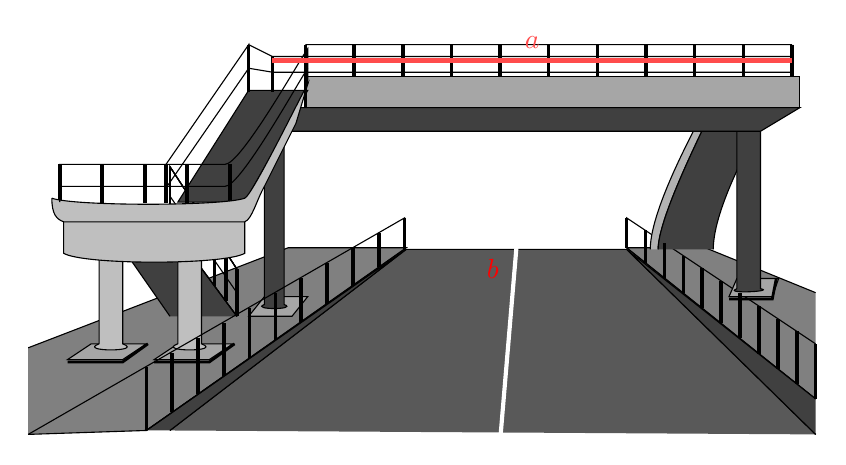
\begin{tikzpicture}
\draw[fill=gray]
(-5,-1.55)--(-1.7,-0.28)--(-0.2,-0.28)--(-3.5,-2.6)--(-5,-2.65);
\draw[fill=gray]
(5,-2.2)--(2.6,-0.28)--(3.6,-0.28)--(5,-0.85);
\draw (5,-2.2)--(2.6,-0.28)--(2.6,0.1)--(5,-1.5);
\draw[fill=gray!70!black]
(-3.2,-2.6)--(-0.2,-0.3)--(2.6,-0.3)--(5,-2.65);
\draw[fill=gray!50!black]
(-3.5,-2.6)--(-0.2,-0.3)--(-3.2,-2.6);
\draw[fill=gray!50!black]
(5,-2.2)--(2.6,-.3)--(5,-2.65);
\draw[fill=gray!60!white] (3,-0.3)..controls++(90:0.4)and++(-110:0.1)..(3.6,1.3)--(3.6,1.5)..controls++(-110:0.1)and++(90:0.55)..(2.9,-0.3);
\draw[fill=gray!50!black] (3,-0.3)..controls++(90:0.4)and++(-110:0.1)..(3.6,1.3)--(4.3,1.3)..controls++(-110:0.1)and++(90:0.55)..(3.7,-0.3);
\draw[fill=gray!70!white] (3.9,-.9)--(4.45,-.9)--(4.53,-0.67)--(4,-0.67)--cycle;
\draw[fill=gray!50!black] (4,-0.8)..controls++(-160:0.2)and++(-10:0.2)..(4.3,-0.8)--(4.3,1.3)--(4,1.3)--(4,-0.8);
\draw[line width=1pt] (3.9,-0.93)--(4.45,-0.93)--(4.5,-0.67);

\draw[white,line width=1.5pt](1,-2.65)--(1.2,-0.28);
\draw[fill=gray!50!black]
(-2.35,-1.15)--(-3.2,0)--(-4,0)--(-3.2,-1.15);
\draw (-2.35,-1.15)--(-2.35,-0.55)--(-3.2,0.75)--(-3.2,0);
\draw (-2.35,-1.15)--(-2.35,-0.55)foreach \i in{0,1,2}{coordinate[pos=\i/2](E\i)};
\draw (-3.2,0)--(-3.2,.75)foreach \i in{0,1,2}{coordinate[pos=\i/2](F\i)};
\foreach \i in{0,1,2}
\draw (E\i)--(F\i);
\draw (-2.35,-1.15)--(-2.35,-0.55)--(-3.2,0.75)--(-3.2,0);
\draw (-2.35,-1.15)--(-3.2,0)foreach \i in{0,1,2,...,6}{coordinate[pos=\i/6](G\i)};
\draw (-2.35,-0.55)--(-3.2,0.75)foreach \i in{0,1,2,...,6}{coordinate[pos=\i/6](H\i)};
\foreach \i in{0,1,2}
\draw[line width=1.3pt] (G\i)--(H\i);
\draw[fill=gray!70!white] (-4.5,-1.7)--(-3.8,-1.7)--(-3.5,-1.5)--(-4.2,-1.5)--cycle;
\draw[line width=1pt] (-4.5,-1.73)--(-3.8,-1.73)--(-3.48,-1.5);
\draw[fill=gray!50!white] (-4.1,-1.5)..controls++(-160:0.3)and++(-20:0.3)..(-3.8,-1.5)--(-3.8,-0.4)--(-4.1,-0.4)--(-4.1,-1.5);
\draw[fill=gray!70!white] (-3.4,-1.7)--(-2.7,-1.7)--(-2.4,-1.5)--(-3.1,-1.5)--cycle;
\draw[line width=1pt] (-3.4,-1.73)--(-2.7,-1.73)--(-2.38,-1.5);
\draw[fill=gray!70!white] (-2.2,-1.15)--(-1.65,-1.15)--(-1.45,-0.9)--(-2,-0.9)--cycle;
\draw[fill=gray!50!black]
(-2,1.2)--(4.3,1.2)--(4.8,1.5)--(-2,1.5) (-2,1.2)--(-2,-1)..controls++(-160:0.2)and++(-20:0.2)..(-1.75,-1)--(-1.75,1.2);
\draw [fill=gray!70!white]  (-1.5,1.5)--(4.8,1.5)--(4.8,1.9)--(-1.5,1.9);
\draw[fill=gray!50!black] (-2.2,1.72)--(-1.45,1.72)--(-2.25,0.3)--(-3.1,0.3)--cycle;
\path (-4.6,0.78)--(-2.44,0.78) foreach \i in{0,1,2,...,4}{coordinate[pos=\i/4](I\i)};
\path (-4.6,0.29)--(-2.44,0.29) foreach \i in{0,1,2,...,4}{coordinate[pos=\i/4](J\i)};
\foreach \i in{0,1,2,...,4}
\draw[line width=1.3pt] (I\i)--(J\i);
\draw (-3.25,0.29)--(-3.25,0.78)--(-2.2,2.3)--(-2.2,1.7)(-3.25,0.48)--(-2.2,2);
\draw[line width=1.3pt]  (-3.25,0.29)--(-3.25,0.78);
\draw [fill=gray!50!white](-3.1,-1.5)..controls++(-160:0.3)and++(-20:0.3)..(-2.8,-1.5)--(-2.8,-0.4)--(-3.1,-0.4)--(-3.1,-1.5);
\draw[fill=gray!50!white] (-4.55,0.05)--(-4.55,-0.35)..controls++(-30:0.3)and++(-150:0.3)..(-2.25,-0.35)--(-2.25,0.05);
\draw[fill=gray!50!white] (-4.7,0.35)..controls++(-90:0.2)and++(160:0.1)..(-4.55,0.05)--(-2.25,0.05)..controls++(20:0.1)and++(-120:0.2)..(-2,0.5)--(-1.6,1.3)--(-1.45,1.8)..controls++(-120:0.2)and++(20:0.1)..(-2.25,0.35)..controls++(-160:0.3)and++(-20:0.3)..(-4.7,0.35);
\draw (-4.6,0.3)--(-4.6,0.78)--(-2.5,0.78)..controls++(0:0.2)and++(-125:0.2)..(-1.45,2.25)--(-1.45,1.8);
\draw (-4.6,0.5)--(-2.5,0.5)..controls++(0:0.2)and++(-125:0.2)..(-1.45,2);
\path (-3.5,-2.6)--(-0.22,-0.3)	foreach \i in{0,1,2,...,10}{coordinate[pos=\i/10](A\i)};
\path (-3.5,-1.8)--(-.22,0.1)foreach \i in{0,1,2,...,10}{coordinate[pos=\i/10](B\i)};
\foreach \i in{0,1,2,...,10}
\draw[line width=1.3pt] (A\i)--(B\i);
\path (5,-2.2)--(2.6,-0.28)	foreach \i in{0,1,2,...,10}{coordinate[pos=\i/10](C\i)};
\path (5,-1.5)--(2.6,0.1)foreach \i in{0,1,2,...,10}{coordinate[pos=\i/10](D\i)};
\foreach \i in{0,1,2,...,10}
\draw[line width=1.3pt] (C\i)--(D\i);
\draw (-3.5,-2.6)--(-0.22,-0.3)--(-.22,0.1)--(-5,-2.65);
\draw[line width=1.3pt] (-1.48,1.5)--(-1.48,2.3)(-2.2,1.7)--(-2.2,2.3)(-1.9,2.15)--(-1.9,1.7)(4.7,2.3)--(4.7,1.9);
\draw (-2.2,2.3)--(-1.9,2.15)--(4.7,2.15)(-1.48,2.3)--(4.7,2.3)(-2.2,2)--(-1.9,1.95)--(4.7,1.95);
\path (-1.48,1.9)--(4.7,1.9)	foreach \i in{0,1,2,...,10}{coordinate[pos=\i/10](M\i)};
\path (-1.48,2.3)--(4.7,2.3)foreach \i in{0,1,2,...,10}{coordinate[pos=\i/10](N\i)};
\foreach \i in{0,1,2,...,10}
\draw[line width=1.3pt] (M\i)--(N\i);
\draw[red!70,line width=1.7pt] (-1.9,2.1)--(4.7,2.1)node[pos=0.5,above]{$a$};
\draw[red] (1.1,-0.8)node[above left]{$b$};
\end{tikzpicture}
\end{center}
\par \shortans{2}
\loigiai{
Vì tay vịn cầu song song với mặt đường và đường kẻ chia làn đường nằm trên mặt đường nên khoảng cách giữa hai đường thẳng $a$ và $b$ chính bằng khoảng cách từ đường thẳng $a$ xuống mặt đường.\\
Khoảng cách giữa hai đường thẳng $a$ và $b$ bằng $3{,}5+0{,}9=4{,}4$ (m).
}
\end{ex}

\begin{ex}%[1H8V5-4]
Cho hình chóp $S.ABCD$ có $SD=x$ và tất cả các cạnh còn lại bằng $1$. Biết $SD$ tạo với mặt phẳng $(ABCD)$ góc $60^\circ$. Tính khoảng cách giữa hai đường thẳng $AC$, $SB$ (kết quả làm tròn đến hàng phần trăm).
\shortans[oly]{$0{,}43$}
\loigiai{\begin{center}
\begin{tikzpicture}[scale=.7, font=\footnotesize, line join=round, line cap=round, >=stealth]
\path (0,0) coordinate (A) (-2,-2) coordinate (B) (4,-2) coordinate (C) (6,0) coordinate (D) (2,4) coordinate (S) (2,-1) coordinate (O) (0,1) coordinate (K);
\draw[dashed] (S)--(O) (S)--(A)--(D)--(B)--(A)--(C) (O)--(K);
\draw (S)--(B)--(C)--(D)--(S)--(C)--(D);
\foreach \x/\y in {S/90,A/-90,B/180,C/-60,D/0,O/-90,K/180}{\fill (\x)node[shift={(\y:3mm)}]{$\x$}circle(1.2pt);}
\draw pic[draw, angle radius = 12pt, "$60^\circ$", angle eccentricity = 1.5]{ angle = S--D--B};
\draw[thin] pic[draw, angle radius = 6pt]{right angle = O--K--S};
\end{tikzpicture}
\end{center}
Ta có $ABCD$ là hình thoi, gọi $O=AC\cap BD$ trong mặt phẳng $(ABCD)$. Khi đó $O$ là trung điểm của $AC$ và $BD$.\\
Do $AB=BC=1$ nên $\triangle ABC$ cân tại $B$. Suy ra $BO$ là đường trung trực của $\triangle ABC$.\\
Hình chóp $S.ABC$ có $SA=SB=SC=1$ nên hình chiếu $H$ của $S$ lên mặt phẳng $(ABC)$ nằm trên đường trung trực $BO$ của $\triangle ABC$.\\
Do đó $\big(SD,(ABCD)\big)=\widehat{SDH}=60^\circ$.\\
Tam giác $SBD$ cân tại $S$ có $\widehat{SDB}=60^\circ$ nên $\triangle SBD$ đều. Do đó $H\equiv O$ và $x=SB=BD=1$.\\
Khi đó $SO=\dfrac{\sqrt{3}}{2}$ và $BO=\dfrac{1}{2}$.\\
Trong mặt phẳng $(SBD)$, dựng $OK\perp SB$ ($K\in SB$). Dễ chứng minh được $AC\perp (SBD)$, từ đó suy ra $OK$ là đoạn vuông góc chung của hai đường thẳng $AC$ và $SB$.\\
Do đó $d(SB,AC)=OK=\dfrac{SO\cdot BO}{\sqrt{SO^2+BO^2}}=\dfrac{\sqrt{3}}{4}=\approx0{,}43$.
}
\end{ex}

\begin{ex}%[1H8V5-3]
\immini{Mở một mô hình kim tự tháp hình chóp tứ giác đều có chiều cao bằng $4$ và trải nó trên mặt phẳng ta được hình dạng như hình bên. Biết $TH=11$. $H$ là trung điểm của một cạnh đáy. Hỏi khoảng cách từ tâm của đáy kim tự tháp đến mặt bên của kim tự tháp bằng bao nhiêu?
\shortans{$2{,}4$}}{
\begin{tikzpicture}[line join=round, line cap=round,>=stealth,font=\footnotesize,scale=0.6]
\def\d{2}
\path
(0,0) coordinate (A)
(150:\d) coordinate (Q)
(0:\d) coordinate (B)
++(30:\d) coordinate (N)
(90:\d) coordinate (D)
++(60:\d) coordinate (P)
($(D)+(B)-(A)$) coordinate (C)
(-60:\d) coordinate (M)
(0:\d/2) coordinate (H)node[below]{$H$};
\draw
(A)--(B)--(C)--(D)--(A)--(M)--(B)--(N)--(C)--(P)--(D)--(Q)--(A) (P)--(H);
\pic[draw,angle radius=0.3cm]{right angle=B--H--P};
\end{tikzpicture}
}
\loigiai{
\begin{center}
\begin{tikzpicture}[line join=round, line cap=round,>=stealth,font=\footnotesize,scale=0.6]
\path
(0,0) coordinate (A)
(0:4) coordinate (D)
(-140:3) coordinate (B)
($(B)+(D)-(A)$) coordinate (C)
($(A)!0.5!(C)$) coordinate (O)
++(90:4) coordinate (T)
($(D)!0.5!(C)$) coordinate (K)
($(A)!0.5!(B)$) coordinate (H)
($(T)!(O)!(K)$) coordinate (E)
;
\draw(T)--(B) (T)--(C) (T)--(D) (B)--(C)--(D) (T)--(K);
\draw[dashed,thin](T)--(A) (A)--(B) (A)--(D) (A)--(C) (B)--(D) (T)--(O)--(E) (K)--(H);
\pic[draw,angle radius=0.3cm]{right angle=T--O--H} pic[draw,angle radius=0.3cm]{right angle=T--E--O};
\foreach \i/\g in {T/90,A/135,B/-90,C/-90,D/0,O/-90,K/-90,E/45,H/90}{\draw[fill=black](\i) circle (1pt) ($(\i)+(\g:3mm)$) node[scale=1]{$\i$};}
\end{tikzpicture}
\end{center}
Ta mô hình hóa bài toán như hình vẽ.\\
Gọi $K$ là trung điểm của $CD$.\\
Gọi độ dài cạnh đáy của kim tự tháp là $2x$ $ (\text{với }2x<11)$.\\
Vì $TK+KH=11\Rightarrow KH=11-2x$.\\
Áp dụng định lí Pythagore cho $\triangle TOK$ ta có
\[TK^2=TO^2+KO^2 \Leftrightarrow (11-2x) ^2=x^2+4^2.\]
Suy ra phương trình $3x^2-44x+105=0 \Rightarrow \hoac{&x=3\\&x=\dfrac{35}{3}\quad(\text{loại}).}$\\
Hạ $OE\perp TK$.\\
Suy ra $OE \perp (TCD)$.\\
Hay $\mathrm{d}\big(O,(TCD)\big)=OE=\dfrac{OK\cdot OT}{\sqrt{OK^2+OT^2}}=\dfrac{4\cdot 3}{\sqrt{4^2+3^2}}=\dfrac{12}{5}=2{,}4$.
}
\end{ex}

\begin{ex}%[1H8V5-4]
Cho hình chóp $S.ABCD$ có đáy $ABCD$ là hình chữ nhật, $SA\perp (ABCD)$ và $AB=$, $AD=\sqrt{3}$, góc giữa mặt phẳng $(SBD)$ và $(ABCD)$ bằng $60^\circ$. Biết khoảng cách giữa hai đường thẳng $AC$ và $SD$ là $a$. Tìm $a$
\shortans{$0{,}75$}
\loigiai{
\immini{
Lấy điểm $E$ thuộc $AB$ sao cho $DE\parallel AC$ thì $AE=AB=1$.\\
Khi đó $AC\parallel (SDE)$ nên $\mathrm{d}(AC,SD)=\mathrm{d}(AC,(SDE))=\mathrm{d}(A,(SDE))$.\\
Kẻ $SH\perp BD$ tại $H$ thì ta có $(SAH)\perp BD\Rightarrow AH\perp BD$.\\
Khi đó $((SBD),(ABCD))=(AH,SH)=\widehat{SHA}=60^\circ$.\\
Lại có $\dfrac{1}{AH^2}=\dfrac{1}{AB^2}+\dfrac{1}{AD^2}=\dfrac{4}{3}\Rightarrow AH=\dfrac{\sqrt{3}}{2}$,\\
nên $SA=AH\cdot\tan\widehat{SHA}=AH\cdot\tan60^\circ=\dfrac{3}{2}$.\\
Trong tứ diện vuông $A.SDE$ kẻ đường cao $AK\perp(SDE)$, khi đó\[\dfrac{1}{AK^2}=\dfrac{1}{AS^2}+\dfrac{1}{AE^2}+\dfrac{1}{AD^2}=\dfrac{16}{9}\] nên $\mathrm{d}(AC,SD)=\mathrm{d}(A,(SDE))=AK=\dfrac{3}{4}=0{,}75$.
}{\begin{tikzpicture}[>=stealth,line join=round,line cap=round,font=\footnotesize,scale=0.6]
\path (0,0) coordinate (A)
(-2.5,-1.4) coordinate (D)
(5,0) coordinate (B)
($(B)+(D)-(A)$) coordinate (C)
($(A)!0.5!(C)$) coordinate (O)
($(A)+(0,6)$)coordinate (S)
($(A)+(D)-(C)$) coordinate (E)
($(D)!0.5!(E)$) coordinate (I)
($(B)!0.3!(D)$) coordinate (H)
($(S)!0.65!(I)$) coordinate (K)
;
\draw (D)--(E)--(S)--(B)--(C)--(S)--(D)--(C) (S)--(I);
\draw[dashed] (E)--(A)--(H)--(S)--(A)--(B)--(D)--(A)--(C) (K)--(A)--(I);
\foreach \p / \r in {A/65,B/45,C/-45,S/90,H/-80,I/-135,D/-135,K/135,E/135}
\fill (\p) circle (1.2pt) node[shift={(\r:2mm)}]{$\p$};
\pic[draw,angle radius=2mm,angle eccentricity=1.5] {right angle = B--H--S};
\pic[draw,angle radius=2mm,angle eccentricity=1.5] {right angle = D--I--A};
\pic[draw,angle radius=2mm,angle eccentricity=1.5] {right angle = A--K--S};
\foreach \x/\y/\z in {S/H/A} \draw pic[draw,angle radius=3mm]{angle=\x--\y--\z};
\draw ($(H)+(140:1)$)node{$60^\circ$};
\end{tikzpicture}}
}
\end{ex}

\begin{ex}%[1H8V5-4]
Cho hình chóp $S.ABC$ có đáy $ABC$ là tam giác vuông tại $A$, $AB=1$, $SA$ vuông góc với mặt phẳng đáy. Gọi $M$ là trung điểm của $BC$. Biết rằng khoảng cách giữa hai đường thẳng $AC$ và $SM$ bằng $\dfrac{\sqrt{2}}{3}$. Tính $SA$? (Kết quả làm tròn đến hàng phần trăm)
\par
\shortans{$1{,}41$}
\loigiai{
\begin{center}
\begin{tikzpicture}[declare function={a=5; b=0.45*a; h=0.65*a;}, line join=round, line cap=round, >=stealth, scale=1]
\path (0,0) coordinate (A)
(a,0) coordinate (C)
(-45:b) coordinate (B)
($(A)+(0,h)$) coordinate (S);
\path ($(C)!0.5!(B)$) coordinate (M);
\path ($(A)!0.5!(B)$) coordinate (N);
\path ($(S)!0.6!(N)$) coordinate (H);
\draw[dashed] (N)--(M)--(A)--(C);
\draw (N)--(S)--(B) (M)--(S)--(A)--(B)--(C)--(S) (A)--(H);
\foreach \x/\goc in {S/90,A/190,B/-90,C/0,M/-45,N/-135,H/180}
\fill (\x) node[shift={(\goc:7pt)}]{$\x$} circle (1pt);
\end{tikzpicture}
\end{center}
Gọi $N$ là trung điểm của $AB$.\\
Ta có $\heva{&MN\parallel AC \\&MN\subset (SMN)} \Rightarrow AC\parallel (SMN)$.\\
Khi đó $\mathrm{d}(AC,SM)=\mathrm{d}\left(AC,(SMN)\right)=\mathrm{d}\left(A,(SMN)\right)$.\\
Kẻ $AH\perp SN$ ($H\in SN$).\\
Ta có $\heva{&MN\perp AB \\&MN\perp SA} \Rightarrow MN\perp (SAB)\Rightarrow MN\perp AH$.\\
Lại có $\heva{&MN\perp AH \\&SN\perp AH} \Rightarrow AH\perp (SMN)\Rightarrow \mathrm{d}\left(A,(SMN)\right)=AH=\dfrac{\sqrt{2}}{3}$.\\
Xét tam giác vuông $SAN$ vuông tại $A$ có
\[\dfrac{1}{AH^2}=\dfrac{1}{SA^2}+\dfrac{1}{AN^2} \Rightarrow \dfrac{1}{SA^2}=\dfrac{1}{AH^2}-\dfrac{1}{AN^2}=\dfrac{1}{\left(\dfrac{\sqrt{2}}{3} \right)^2}-\dfrac{1}{\left(\dfrac{1}{2}\right)^2}=\dfrac{1}{2} \Rightarrow SA=\sqrt{2}.\]
}
\end{ex}

\begin{ex}%[1H8V5-3]
Cho hình chóp $S.ABCD$ có đáy $ABCD$ là hình chữ nhật, $AB=a, AD=2a\sqrt{3}$. Cạnh bên $SA$ vuông góc với đáy, biết tam giác $SAD$ có diện tích $S=3a^2$. Khi $a=\sqrt{51}$ thì khoảng cách từ $C$ đến $(SBD)$ bằng bao nhiêu?
\shortans[0]{$6$}
\loigiai{
\immini{
Do $S_{SAD}=3a^2=\dfrac{1}{2}\cdot SA\cdot  AD\Rightarrow SA=\dfrac{6a^2}{2a\sqrt{3}}=a\sqrt{3}$.\\
Mặt khác ta có $\mathrm{d}\left(C,(SBD)\right)=\mathrm{d}\left(A,(SBD)\right)$.\\
Kẻ $AH\bot BD$ tại $H$, $AK\bot SH$ tại $K$ $\Rightarrow \mathrm{d}\left(A,(SBD)\right)=AK$.\\
$BD=\sqrt{AB^2+AD^2}=a\sqrt{13}$\\
$ \Rightarrow AH=\dfrac{AB\cdot AD}{BD}=\dfrac{a\cdot 2a\sqrt{3}}{a\sqrt{13}}=\dfrac{2a\sqrt{39}}{13}$.\\
$\Rightarrow AK=\dfrac{SA.AH}{\sqrt{SA^2+AH^2}}=\dfrac{a\sqrt{3}\cdot \dfrac{2a\sqrt{39}}{13}}{\sqrt{\left(a\sqrt{3} \right)^2+\left(\dfrac{2a\sqrt{39}}{13} \right)^2}}=\dfrac{2a\sqrt{51}}{17}$.\\
}{
\begin{tikzpicture}[rotate=0, scale=0.8, line join=round, line cap=round, >=stealth,line width=.8pt]
\coordinate (A) at (0,0);
\coordinate (S) at (0,4);
\coordinate (B) at (-1.6,-2);
\coordinate (D) at (5,0);
\coordinate (C) at ($(B)+(D)-(A)$);
\coordinate (H) at ($(B)!0.4!(D)$);
\coordinate (K) at ($(S)!0.7!(H)$);
\draw(S)--(B)--(C)--(D)--(S)--(C);
\draw[dashed](S)--(A)--(B)--(D)--(A)--(H)--(S) (A)--(K);
\foreach \x/\g in {A/180,B/-120,C/0,D/0,H/-90,K/20,S/90}\fill[black](\x) circle (1pt)($(\x)+(\g:2.5mm)$) node[scale = 0.7]{$\x$};
\draw pic[draw,angle radius=2mm] {right angle = A--H--B};
\draw pic[draw,angle radius=2mm] {right angle = S--K--A};
\path (A)--(D) node[midway,above,sloped,pos=.5] {\tiny $2a\sqrt{3}$} ;
\path (S)--(A) node[midway, below,sloped,pos=.6] {\tiny $a\sqrt{3}$} ;
\path (A)--(B) node[midway,above,sloped,pos=.4] {\tiny $a$} ;
\end{tikzpicture}
}
Vậy $\mathrm{d}\left(C,(SBD)\right)=\mathrm{d}\left(A,(SBD)\right)=\dfrac{2a\sqrt{51}}{17} \stackrel{a=\sqrt{51}}{\to} \mathrm{d}\left(C,(SBD)\right)=6$.
}
\end{ex}

\begin{ex}%[1H8V5-4]
Cho hình tứ diện $OABC$ có đáy $OBC$ là tam giác vuông tại $O$; $OB = 1$ và $OC = \sqrt{3}$. Cạnh $OA$ vuông góc với mặt phẳng $(OBC)$; $OA = \sqrt{5}$ và gọi $M$ là trung điểm của $BC$. Tính khoảng cách giữa hai đường thẳng $AB$ và $OM$ (Kết quả làm tròn đến hàng phần trăm).

\par \shortans[0]{0,77}
\loigiai{
\immini{Dựng $D$ sao cho $BD\parallel  OM$ và $OM$ là đường trung bình của tam giác $BCD$.\\
Khi đó ta có $OM\parallel (ABD) \Rightarrow \mathrm{d}(OM,AB) = \mathrm{d}(OM, (ABD)) =\mathrm{d}(O, (ABD))$.\\
Kẻ $OH \perp BD$. Lại có $BD \perp OA$ (do $\heva{& OA \perp (OBC) \\& BD \subset (OBC)}$) suy ra $BD \perp (AOH)$.\\
Suy ra $(AOH) \perp (ABD)$ theo giao tuyến $AH$.\\
Trong $(AHO)$, kẻ $OK \perp AH$ suy ra $OK \perp (ABD) \Leftrightarrow OK = \mathrm{d}(O, (ABD))$.\\
Trong $\triangle AHO$:
\begin{eqnarray*}
\dfrac{1}{OK^2}=  \dfrac{1}{OH^2} + \dfrac{1}{OA^2}
=  \dfrac{1}{OD^2} + \dfrac{1}{OB^2} + \dfrac{1}{OA^2}
=  \dfrac{1}{3\cdot1^2} + \dfrac{1}{3\cdot1^2} + \dfrac{1}{1^2}.
\end{eqnarray*}
Suy ra $OK = \dfrac{\sqrt{15}}{5}$ hay $\mathrm{d}(OM,AB) = \dfrac{\sqrt{15}}{5} \approx 0{,}77$.
}{\begin{tikzpicture}[>=stealth,line join=round,line cap=round,font=\footnotesize,scale=0.9]
\path (0,0) coordinate (O)
(-1,-1) coordinate (B)
(4,0) coordinate (C)
($(O)+(0,3)$)coordinate (A)
($(B)!0.5!(C)$)coordinate (M)
($(C)!2!(O)$)coordinate (D)
($(B)!0.4!(D)$)coordinate (H)
($(A)!0.5!(H)$)coordinate (K)
;
\draw (A)--(B)--(C)--(A)--(H) (B)--(D)--(A);
\draw[dashed] (A)--(O)--(C) (H)--(O)--(B) (M)--(O)--(D) (O)--(K);
\pic[draw,angle radius=1.5mm,angle eccentricity=1.5] {right angle = O--K--A};
\pic[draw,angle radius=1.5mm,angle eccentricity=1.5] {right angle = O--H--B};
\pic[draw,angle radius=1.5mm,angle eccentricity=1.5] {right angle = A--O--C};
\foreach \p / \r in {A/90,B/-135,C/45,O/-90,M/-45,D/180,H/-90,K/180}
\fill (\p) circle (1pt) node[shift={(\r:3mm)}]{$\p$};
\end{tikzpicture}}
}
\end{ex}

\begin{ex}%[1H8C5-6]
Một bể cá đầy nước có dạng hình hộp chữ nhật $ABCD.EFGH$ với $AB = 6$ (dm), $AD = 8$ (dm) và cạnh bên bằng $10$ (dm). Một chú cá bơi theo những đoạn thẳng từ điểm $G$ đến chạm mặt đáy của hồ, rồi từ điểm đó bơi đến vị trí diểm $M$ là trung điểm của $AF$ được mô hình hóa như sau
\begin{center}
\begin{tikzpicture}[line join = round, line cap=round,>=stealth,font=\footnotesize,scale=0.8]
\path
(0,0) coordinate (A)
(1.5,1.5) coordinate (B)
(6.5,1.5) coordinate (C)
(5,0) coordinate (D)
;
\foreach \x/\y in {A/E,B/F,C/G,D/H}
\path
($(\x)+(0,3)$) coordinate (\y)
;
\path ($(A)!.5!(F)$) coordinate (M);
\fill[gray!30] (A) -- (B) -- (C) -- (D) --cycle;
\draw
(A) -- (D) -- (C) -- (G) -- (F) -- (E) -- (H) -- (G)
(A) -- (E)
(D) -- (H)
;
\draw[dashed]
(A) -- (B) -- (C)
(A) -- (F) -- (B)
;
\fill
(A) circle(1pt) node[below]{$A$}
(B) circle(1pt) node[left]{$B$}
(C) circle(1pt) node[below]{$C$}
(D) circle(1pt) node[below]{$D$}
(E) circle(1pt) node[above]{$E$}
(F) circle(1pt) node[above]{$F$}
(G) circle(1pt) node[above]{$G$}
(H) circle(1pt) node[above]{$H$}
(M) circle(1pt) node[left]{$M$}
;
\end{tikzpicture}
\end{center}
Để đường đi ngắn nhất thì chú cá bơi đến điểm dưới đáy hồ cách $BA$ và $BC$ những đoạn thẳng bằng $a$ và $b$. Khi đó tổng $D = 3a + 6b$ bằng bao nhiêu? (kết quả làm tròn đến hàng đơn vị)
\par\shortans[]{$20$}
\loigiai{
Gọi $I$ là trung điểm của $AB$.\\
Khi đó $IC = \left(MICG \right) \cap \left(ABCD \right)$.\\
Giả sử con cá bơi tới điểm $K \in HC$.\\
Khi đó quãng đường con cá bơi là $GK + KM$.\\
Ta có $IC = \sqrt{IB^2 + BC^2} = \sqrt{3^2 + 8^2} = \sqrt{73}$ m.\\
Đặt $KC =x \,  \left(x > 0 \right)$.
\begin{center}
\begin{tabular}{cc}

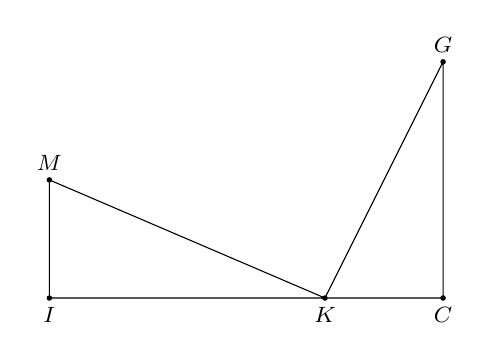
\begin{tikzpicture}[line join = round, line cap=round,>=stealth,font=\footnotesize,scale=1]
\path
(0,0) coordinate (I)
(5,0) coordinate (C)
(3.5,0) coordinate (K)
(0,1.5) coordinate (M)
(5,3) coordinate (G)
;
\draw
(G) -- (K) -- (M) -- (I) -- (C) -- (G)
;
\fill
(G) circle(1pt) node[above]{$G$}
(K) circle(1pt) node[below]{$K$}
(C) circle(1pt) node[below]{$C$}
(M) circle(1pt) node[above]{$M$}
(I) circle(1pt) node[below]{$I$}
;
\end{tikzpicture} &
\begin{tikzpicture}[line join = round, line cap=round,>=stealth,font=\footnotesize,scale=1]
\path
(0,0) coordinate (B)
(3.5,0) coordinate (I)
(0,3) coordinate (C)
($(C)!0.4!(I)$) coordinate (K)
($(B)!(K)!(I)$) coordinate (N)
($(B)!(K)!(C)$) coordinate (L)
;
\draw
(I) -- (B) -- (C) -- (I)
(L) -- (K) -- (N)
;
\fill
(C) circle(1pt) node[above]{$G$}
(K) circle(1pt) node[above]{$K$}
(I) circle(1pt) node[below]{$C$}
(L) circle(1pt) node[left]{$L$}
(B) circle(1pt) node[below]{$B$}
(N) circle(1pt) node[below]{$N$}
;
\path (B) pic[draw, angle radius=6]{right angle=I--B--C};
\path (B) pic[draw, angle radius=6]{right angle=I--N--K};
\path (B) pic[draw, angle radius=6]{right angle=K--L--C};
\end{tikzpicture}
\end{tabular}
\end{center}
Khi đó $GK + KM = \sqrt{x^2 +10^2} +\sqrt{5^2 + \left(\sqrt{73} - x \right)^2}$.\\
Ta tìm giá trị nhỏ nhất của $f(x) = \sqrt{x^2 +10^2} +\sqrt{5^2 + \left(\sqrt{73} - x \right)^2}$.\\
Theo bất đẳng thức Minkowski ta có
\[\sqrt{x^2 + 10^2} + \sqrt{\left(\sqrt{73} - x \right)^2 + 5^2} \geq \sqrt{\left(x + \sqrt{73} - x \right)^2 + \left(10+5 \right)^2} = \sqrt{298}.\]
Dấu \lq\lq $=$\rq\rq \, xảy ra khi và chỉ khi $\dfrac{x}{\sqrt{73} - x} = \dfrac{10}{5} \Leftrightarrow x = 5{,}696$.\\
Khi đường đi ngắn nhất thì $KC = 5{,}696$.\\
Kẻ $KL \perp BC$, $KN \perp BI$ $\left(L \in BC, N \in BI \right)$.\\
Ta có $\dfrac{KL}{BI} = \dfrac{KC}{CI} \Rightarrow \dfrac{KL}{3} = \dfrac{5{,}696}{\sqrt{73}} \Rightarrow KL \approx 2$ m.
\[\dfrac{KN}{BC} = \dfrac{KI}{IC} \Rightarrow = \dfrac{KI \cdot BC}{IC} = \dfrac{\left(\sqrt{73} - 5{,}696 \right) \cdot 8}{\sqrt{73}} \approx 2{,}67.\]
Vậy $D =3a + 6b = 3 \cdot 2{,}67 + 6 \cdot 2 = 20$ m.
}
\end{ex}

\begin{ex}%[1H8C5-4]
Cho hình lăng trụ đứng $ABC.A'B'C'$ có đáy $ABC$ là tam giác đều có cạnh bằng $1$ và cạnh bên $AA'=\sqrt{2}$. Tính khoảng cách giữa hai đường thẳng $A'B$ và $B'C$ (\textit{làm tròn kết quả đến hàng phần trăm}).
\par
\shortans[0]{0,47}
\loigiai{
\begin{center}
\begin{tikzpicture}[scale=1, font=\footnotesize, line join=round, line cap=round, >=stealth]
\foreach \x/\y/\z/\t in {A/0/0/180,B/4/0/-90,C/2.5/-1.5/-90,D/8/0/0,A'/0/4/90,B'/4/4/90,C'/2.5/2.5/90} {
\coordinate (\x) at (\y,\z);
\draw[fill=black] (\x) circle (1pt) ($(\x)+(\t:3mm)$) node {$\x$};
}
\coordinate (K) at ($(C)!0.5!(D)$);
\coordinate (H) at ($(B')!0.7!(K)$);
\foreach \x/\y in {K/-80,H/0} {\draw[fill=black] (\x) circle (1pt) ($(\x)+(\y:3mm)$) node {$\x$};}
\draw (A)--(A')--(B')--(D)--(C)--(A) (C)--(C')--(A') (C')--(B')--(C) (B')--(K);
\draw[dashed] (A)--(D) (A')--(B)--(B') (C)--(B)--(K) (B)--(H);
\tkzMarkRightAngles(B,K,C B,H,B')
\end{tikzpicture}
\end{center}
Gọi $D$ là điểm đối xứng với $A$ qua $B$ thì khi đó $A'B\parallel B'D$.\\
Suy ra $d\left(A'B,B'C\right)=d\left(A'B,(B'CD)\right)=d\left(B,(B'CD)\right)$.\\
kẻ $BK\perp CD$ $(K\in CD)$, ta có $BA=BC=BD$ nên $\triangle ACD$ vuông tại $C$ mà $BK\parallel AC$.\\
Mặt khác $B$ là trung điểm của $AD$ nên $K$ là trung điểm của $CD$ và $BK=\dfrac{1}{2}AC=\dfrac{1}{2}$.\\
Kẻ $BH\perp B'K$ tại $H$ thì ta suy ra được $d\left(B,(B'CD)\right)=BH$.\\
Ta có $\dfrac{1}{BH^2}=\dfrac{1}{BK^2}+\dfrac{1}{BB'^2}=\dfrac{4}{1^2}+\dfrac{1}{2\cdot 1^2}=\dfrac{9}{2}\Rightarrow BH=\dfrac{\sqrt{2}}{3}$.\\
Vậy $d\left(A'B,B'C\right)=\dfrac{\sqrt{2}}{3}\approx 0{,}47$
}
\end{ex}

\begin{ex}%[1H8C5-4]
Cho hình chóp $S.ABCD$ có $SA\perp (ABCD)$, $SA=3$, $ABCD$ là hình vuông cạnh bằng $1$. Tính khoảng cách giữa hai đường thẳng $AC$ và $SB$ (kết quả làm tròn đến hàng phần trăm).
\shortans{$0{,}69$}
\loigiai{
\begin{center}
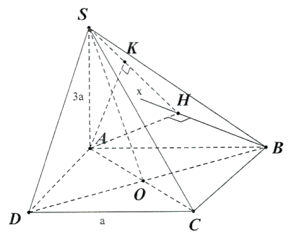
\includegraphics[scale=0.9]{images/Otc7Cau5TLN}
\end{center}
Dựng $Bx\parallel AC\Rightarrow AC\parallel (SBx)$.\\
Suy ra $\mathrm{d}(AC,SB)=\mathrm{d}(AC,(SBx))=\mathrm{d}(A,(SBx))$.\\
Dựng và chứng minh được $\mathrm{d}(A,(SBx))=AK$.\\
Ta có $\triangle AHB$ vuông cân tại $H$ nên $AH=\dfrac{AB}{\sqrt{2}}=\dfrac{1}{\sqrt{2}}$.\\
Ta có $AK=\dfrac{1}{\sqrt{\dfrac{1}{SA^2}+\dfrac{1}{AH^2}}}=\dfrac{1}{\sqrt{1}+\dfrac{1}{(3)^2}}=\dfrac{3\sqrt{19}}{19}$.\\
Vậy $\mathrm{d}(AC,SB)=\dfrac{3\sqrt{19}}{19}\approx0{,}69$.
}
\end{ex}

\begin{ex}%[1H8C5-4]
Cho hình chóp $S . A B C D$ có đáy $A B C D$ là hình vuông cạnh $a, S D=\dfrac{a \sqrt{17}}{2}$, hình chiếu vuông góc $H$ của $S$ trên mặt phẳng $(A B C D)$ là trung điểm của đoạn $A B$. Gọi $K$ là trung điểm của đoạn $A D$. Khi $a=5 \sqrt{3}$ khoảng cách $h$ giữa hai đường thẳng $H K$ và $S D$ bằng bao nhiêu?
\shortans[0]{$1$}
\loigiai{
\immini
{
Ta có $S H \perp(A B C D) \Rightarrow S H \perp H D$.\\
Suy ra $S H=\sqrt{S D^2-H D^2}=\sqrt{S D^2-\left(H A^2+D A^2\right)}=\sqrt{\dfrac{17 a^2}{4}-\left(\dfrac{a^2}{4}+a^2\right)}=a \sqrt{3}$.\\
Do $H K \parallel B D \Rightarrow H K \parallel (S B D) \Rightarrow d(H K, S D)=d(H K,(S B D))=d(H,(S B D))$ (1)\\
Kẻ $H E \perp B D(E \in B D)$, suy ra: $(S H E) \perp(S B D)$ và $(S H E) \cap(S B D)=S E$.\\
Kẻ $H F \perp S E(F \in S E)$, khi đó: $H F \perp(S B D)$.\\
Suy ra: $d(H,(S B D))=H F$ (2)\\
Xét tam giác $H E B$, ta có: $H E=H B \sin \widehat{H B E}=\dfrac{a}{2} \cdot \sin 45^\circ=\dfrac{a}{2 \sqrt{2}}$.
}
{
\begin{tikzpicture}[line join=round,line cap=round,line width=.6pt,font=\footnotesize,scale=1]
\coordinate[label=below left:$B$] (B) at (0,0);
\coordinate[label=left:$A$] (A) at (1,2);
\coordinate[label=below right:$C$] (C) at (4,0);
\coordinate[label=above right:$D$] (D) at ($(C)-(B)+(A)$);
\coordinate[label=left:$H$] (H) at ($(A)!1/2!(B)$);
\coordinate[label=above left:$S$] (S) at ($(H)+(90:4)$);
\coordinate[label=above:$K$] (K) at ($(A)!0.5!(D)$);
\coordinate[label = below right:$E$] (E) at ($(B)!1/2.5!(D)$);
\coordinate[label = right:$F$] (F) at ($(S)!2/3!(E)$);

\draw (B)--(C)--(D)--(S)--cycle (S)--(C);
\draw[dashed] (A)--(D)--(B) (H)--(S)--(A)--(B) (D)--(H)--(E)--(F)--(S) (F)--(H)--(K);
\draw ($ (H)!5pt!(A)$)--($(H)!2!($($(H)!5pt!(A)$)!.5!($(H)!5pt!(S)$)$)$)--($(H)!5pt!(S)$);
\fill (A)circle(1.5pt) (B)circle(1.5pt) (C)circle(1.5pt) (D)circle(1.5pt) (S)circle(1.5pt) (H)circle(1.5pt) (K)circle(1.5pt) (E)circle(1.5pt) (F)circle(1.5pt);
\foreach \x/\dinh/\y in {H/E/B,H/F/E} \draw[fill = gray!50] ($(\dinh)!5pt!(\x)$)--($(\dinh)!5pt!(\x)+(\dinh)!5pt!(\y)-(\dinh)$)--($(\dinh)!5pt!(\y)$)--(\dinh)--cycle;
\end{tikzpicture}

}
\noindent
Xét tam giác $S H E$, ta có $: \dfrac{1}{H F^2}=\dfrac{1}{S H^2}+\dfrac{1}{H E^2}=\dfrac{1}{3 a^2}+\dfrac{8}{a^2}=\dfrac{25}{3 a^2} \Rightarrow H F=\dfrac{a \sqrt{3}}{5}$ (3)\\
Từ (1),(2),(3) suy ra: $d(H K, S D)=\dfrac{a \sqrt{3}}{5} \xrightarrow{a=5 \sqrt{3}} d(H K, S D)=1$.
}
\end{ex}

\begin{ex}%[1H8V6-3]
Cho khối chóp $S.ABCD$ có đáy là hình bình hành, $AB=3$, $AD=4$, $\widehat{BAD} =120^\circ$. Cạnh bên $SA=2\sqrt{3}$ vuông góc với mặt phẳng đáy. Gọi $M$, $N$, $P$ lần lượt là trung điểm các cạnh $SA$, $AD$, $BC$. Tính góc giữa hai mặt phẳng $\left(SBC\right)$ và $\left(MNP\right)$.
\par\shortans{$45^\circ$}
\loigiai{
\begin{center}
\begin{tikzpicture}[scale=1, font=\footnotesize, line join=round, line cap=round, >=stealth]
\def\a{3}
\path
(0,0) coordinate (A)
(0:\a) coordinate (D)
(220:0.6*\a) coordinate (B)
($(B)+(D)$) coordinate (C)
(90:0.8*\a) coordinate (S)
($(S)!0.5!(A)$) coordinate (M)
($(A)!0.5!(D)$) coordinate (N)
($(B)!0.5!(C)$) coordinate (P)
($(S)!0.5!(B)$) coordinate (I)
($(B)!0.2!(C)$) coordinate (K)
($(S)+(P)-(C)$) coordinate (J)
($(J)!1.7!(S)$) coordinate (X)node[above]{$x$}
($(S)!1.2!(J)$) coordinate (Y)
($(S)!0.6!(K)$) coordinate (E)
;
\draw (S)--(B)--(C)--(D)--(S)--(C)(X)--(Y)(J)--(P)(S)--(K);
\draw[dashed] (S)--(A)--(B)(A)--(D)(A)--(K)(J)--(N)--(P)(I)--(M)(A)--(E);
\foreach \x/\g in {S/90,A/-60,B/180,C/-80,D/0,M/20,N/60,P/-90,I/180,J/90,K/-90,E/30}\fill[black] (\x) circle (1pt)+(\g:.3)node{$\x$};
\end{tikzpicture}
\end{center}
Ta có $\left(SAD\right)\cap\left(SBC\right)=Sx\parallel AD\parallel BC$\\
Gọi $I$ là trung điểm $SB$ suy ra $\heva{&MI\parallel NP\parallel AB\\
&MI=\dfrac{NP}{2}.}$\\
Dễ dàng chứng minh được $IP$, $MN$, $Sx$ đồng quy tại $J$.\\
Như vậy $I$ là trung điểm của $JP$, $M$ là trung điểm $JN$.\\
Gọi $\alpha $ là góc giữa hai mặt phẳng $\left(SBC\right)$ và $\left(MNP\right)$, suy ra $\sin\alpha=\dfrac{\mathrm{d}\left(M,\left(SBC\right)\right)}{\mathrm{d}\left(M,IP\right)}$.\\
Suy ra $\mathrm{d}\left(M,\left(SBC\right)\right)=\dfrac{1}{2}\mathrm{d}\left(A,\left(SBC\right)\right)$.\\
Hạ $AK\perp BC$, $AE\perp SK\Rightarrow AE\perp\left(SBC\right)\Rightarrow \mathrm{d}\left(A,\left(SBC\right)\right)=AE$.\\
$AK=AB\cdot\sin\widehat{ABK}=3\sin60^\circ=\dfrac{3\sqrt{3}}{2}$.\\
Xét $\triangle SAK$ có
\[\dfrac{1}{AE^2}=\dfrac{1}{AS^2}+\dfrac{1}{AK^2}=\dfrac{1}{12}+\dfrac{4}{27}=\dfrac{75}{324}\Rightarrow AE=\dfrac{6\sqrt{3}}{5}\Rightarrow \mathrm{d}\left(M,\left(SBC\right)\right)=\dfrac{3\sqrt{3}}{5}.\]
Ta có $\mathrm{d}\left(M,PI\right)=\dfrac{1}{2}\mathrm{d}\left(N,PI\right)$.\\
Xét $\triangle ABC$ có $AC^2=AB^2+CB^2-2AB\cdot BC\cdot \cos60^\circ=13\Rightarrow AC=\sqrt{13}$.\\
$JP=2IP=SC=\sqrt{13+12}=55,JN=2MN=SD=2\sqrt{7},PN=AB=3$.\\
$\Rightarrow{S_{\triangle JPN}}=3\sqrt{6}$.\\
Mà $S_{JPN}=\dfrac{1}{2}\mathrm{d}\left(N,JP\right)\cdot JP=\dfrac{6\sqrt{6}}{5}\Rightarrow \mathrm{d}\left(M,IP\right)=\dfrac{3\sqrt{6}}{5}$.\\
Vậy $\sin\alpha=\dfrac{\sqrt{2}}{2}\Rightarrow\alpha=45^\circ$.
}
\end{ex}

\begin{ex}%[1H8V6-5]
Cho hình chóp $S.ABC$ có đáy $ABC$ là tam giác vuông tại $A$, $(SAC)\perp (ABC)$, $AB=3$, $BC=5$. Biết rằng $SA=2\sqrt{3}$ và $\widehat{SAC}=30^\circ$. Khoảng cách (\textit{làm tròn đến hàng phần trăm}) từ $A$ đến mặt phẳng $(SBC)$ bằng
\shortans{$2{,}27$}
\loigiai{
\immini{
Kẻ $SH\perp AC$ tại $H$. Ta có\\
$\heva{&(SAC)\perp (ABC)\\&SH\perp AC\\&(SAC)\cap (ABC)=AC}\Rightarrow SH\perp (ABC)$.\\
$\triangle ABC$ vuông tại $A\Rightarrow AC=\sqrt{BC^2-AB^2}=4$.\\
$\triangle SAH$ vuông tại $H\Rightarrow AH=SA\cdot\cos 30^\circ =3\Rightarrow HC=1$ và $SH=\sqrt{3}$. Khi đó ta có \\$\dfrac{\mathrm{d}(A,(SBC))}{\mathrm{d}(H,(SBC))}=\dfrac{AC}{HC}=4\Rightarrow\mathrm{d}(A,(SBC))=4\mathrm{d}(H,(SBC))$.
}{
\begin{tikzpicture}[scale=.6, font=\footnotesize, line join=round, line cap=round, >=stealth]
\path (0,0)coordinate(A) (2.2,-2)coordinate(C) (5.5,0)coordinate(B) ($(A)!2/3!(C)$)coordinate(H) ($(B)!3/5!(C)$)coordinate(M) ($(S)!.6!(M)$)coordinate(K);
\coordinate (S) at ($(H)+(0,6.6)$);
\foreach \i/\j in {S/90,A/180,B/0,C/-90,H/190,M/-30,K/0}
\draw[fill=black] (\i)node[shift=(\j:.32)]{$\i$}circle(1pt);
\draw[dashed] (K)--(H)--(M) (A)--(B);
\draw (S)--(A)--(C)--(S)--(B)--(C) (H)--(S)--(M);
\pic[draw,angle radius=2mm] {right angle=S--H--C};
\pic[draw,angle radius=2mm] {right angle=H--K--M};
\pic[draw,angle radius=2mm] {right angle=H--M--C};
\end{tikzpicture}
}
\noindent Kẻ $HM\perp BC$ tại $M$, kẻ $HK\perp SM$ tại $K$, ta có\\
$\heva{&BC\perp HM\\&BC\perp SH}\Rightarrow BC\perp (SHM)$.\\
$\heva{&HK\perp SM\\&HK\perp BC}\Rightarrow HK\perp (SBC)\Rightarrow\mathrm{d}(H,(SBC))=HK$.\\
$\triangle MCH\backsim \triangle ACB\Rightarrow \dfrac{MH}{AB}=\dfrac{CH}{BC}\Rightarrow MH=\dfrac{CH}{BC}\cdot AB=\dfrac{3}{5}$.\\
$\triangle SHM$ vuông tại $H$ có $HK\perp SM\Rightarrow HK=\dfrac{SH\cdot HM}{\sqrt{SH^2+HM^2}}=\dfrac{3\sqrt{7}}{14}$.\\
Vậy $\mathrm{d}(A,(SBC))=4HK=4\cdot\dfrac{3\sqrt{7}}{14}=\dfrac{6\sqrt{7}}{7}\approx 2{,}27$.
}
\end{ex}

\begin{ex}%[1H8V6-3]
Cho tứ diện đều $ABCD$. Gọi $\varphi $ là góc giữa hai mặt phẳng $(BCD)$ và $(ABC)$. Tính $\cos \varphi$ (làm tròn đến hàng phầm trăm).
\shortans[]{$0{,}33$}
\loigiai{
\immini{Giả sử tứ diện đều có tất cả các cạnh bằng $x$ \\
Gọi $M$ là trung điểm $BC$ \\
Do tam giác $ABC,DBC$ đều nên $\heva{
&AM\perp BC \\
&DM\perp BC.} $ \\
Do đó $\varphi =(AM;DM)$. \\
Xét tam giác $AMD$ có $AM=DM=\dfrac{x\sqrt{3}}{2}$. \\
Mặt khác
\begin{eqnarray*}
\cos \widehat{AMD} &=&\dfrac{AM^2+MD^2-AD^2}{2\cdot AM\cdot MD}\\
&=&\dfrac{\dfrac{3x^2}{4}+\dfrac{3x^2}{4}-x^2}{2\cdot \dfrac{x\sqrt{3}}{2}\cdot \dfrac{x\sqrt{3}}{2}}\\
&=&\dfrac{\dfrac{1}{2}x^2}{\dfrac{3x^2}{2}}=\dfrac{1}{3}>0.
\end{eqnarray*}
Nên $\cos AMD=\cos (AM;MD)=\cos \varphi $. \\
Vậy $\cos \varphi =\dfrac{1}{3}\approx 0{,}33$.}{\begin{tikzpicture}[line cap=round,line join=round, >=stealth,scale=0.8]
\def \xa{3}
\def \xb{2}
\def \y{5}
\def \z{5}
\coordinate[label=left:{$B$}]  (B) at (0,0);
\coordinate[label=below:{$C$}]  (C) at ($(\xa,-\xb)$);
\coordinate[label=right:{$D$}]  (D) at (7,0);
\coordinate[label=below left:{$M$}]  (M) at ($0.5*(B)+0.5*(C)$);
\coordinate (N) at ($0.7*(M)+0.3*(D)$);
\coordinate[label=above:{$A$}]  (A) at ($(N)+(0,\z)$);
\draw [dashed] (B)--(D)--(M);
\draw[](M)--(A)--(B)--(C)--(D)--(A)--(C);
\foreach \x/\dinh/\y in {A/M/B,D/M/C} \draw[fill = gray!50] ($(\dinh)!3pt!(\x)$)--($(\dinh)!3pt!(\x)+(\dinh)!3pt!(\y)-(\dinh)$)--($(\dinh)!3pt!(\y)$)--(\dinh)--cycle;
\foreach \p in {A,B,C,D,M}
\fill (\p) circle (1.5pt);
\end{tikzpicture} } }
\end{ex}

\begin{ex}%[1H8V6-1]
\immini{Cho hình chóp $S.ABCD$ có đáy $ABCD$ là hình vuông cạnh $a$. Hình chiếu của $S$ lên mặt $(ABCD)$ là trung điểm $H$ của $AB$ và tam giác $SAB$ đều. Gọi $K$ là trung điểm của $AD$, $\alpha$ là góc giữa $SC$ và mặt phẳng $(SHK)$. $\sin \alpha=\dfrac{a}{b}$, với $\dfrac{a}{b}$ tối giản. Tính $a^2+b^2$.
\shortans{$25$}
}
{
\begin{tikzpicture}[>=stealth,line join=round,line cap=round,font=\footnotesize,scale=1]
\path
(0,0) coordinate (A) node[left]{$A$}
(-1.5,-1) coordinate (B) node[below]{$B$}
(4,0) coordinate (D) node[right]{$D$}
($(B)+(D)-(A)$) coordinate (C) node[below]{$C$}
($(A)!.5!(B)$) coordinate (H) node[below right]{$H$}
+(0,3) coordinate (S) node[above]{$S$}
($(A)!.5!(D)$) coordinate (K) node[above]{$K$}
;
\draw (S)--(B)--(C)--(D)--cycle (S)--(C);
\draw[dashed] (S)--(A)--(B) (A)--(D);
\foreach \x in{A,B,C,D,S,H,K}\draw[fill=black] (\x) circle (1pt);
\end{tikzpicture}
}
\loigiai{
\immini{Ta có $\heva{&HK\parallel BD\\&BD\perp AC}\Rightarrow AC\perp HK$.\\
Ta có $\heva{&AC\perp SH\\&AC\perp HK}\Rightarrow AC\perp (SHK)$.\\
Hình chiếu của $SC$ lên $(SHK)$ là $SM$.\\
Suy ra góc giữa $SC$ và $(SHK)$ là góc $\widehat{CSM}=\alpha$.\\
Ta có $HM=\dfrac{BD}{4}=\dfrac{a\sqrt{2}}{4}$.
}
{
\begin{tikzpicture}[>=stealth,line join=round,line cap=round,font=\footnotesize,scale=1]
\path
(0,0) coordinate (A) node[left]{$A$}
(-1.5,-1) coordinate (B) node[below]{$B$}
(4,0) coordinate (D) node[right]{$D$}
($(B)+(D)-(A)$) coordinate (C) node[below]{$C$}
($(A)!.5!(B)$) coordinate (H) node[below]{$H$}
+(0,3) coordinate (S) node[above]{$S$}
($(A)!.5!(D)$) coordinate (K) node[above]{$K$}
;
\path[name path=ac] (A)--(C);
\path[name path=hk] (H)--(K);
\path[name intersections={of= ac and hk,by=M}];
\node[below]at (M){$M$};
\draw (S)--(B)--(C)--(D)--cycle (S)--(C);
\draw[dashed] (S)--(A)--(B) (A)--(D) (A)--(C) (S)--(H)--(K) (S)--(M) (B)--(D);
\foreach \x in{A,B,C,D,S,H,K,M}\draw[fill=black] (\x) circle (1pt);
\end{tikzpicture}
}
\noindent
$SH=\dfrac{a\sqrt{3}}{2}$ với $SH$ là đường cao tam giác đều cạnh $a$.\\
$SM=\sqrt{SH^2+HM^2}=\dfrac{a\sqrt{14}}{4}$.
Ta có $MC=\dfrac{3}{4}AC=\dfrac{3a\sqrt{2}}{4}$.\\
Suy ra $SC=\sqrt{SM^2+MC^2}=a\sqrt{2}$.\\
Vậy $\sin \alpha=\dfrac{MC}{SC}=\dfrac{3}{4}$.\\
Suy ra $a^2+b^2=3^2+4^2=25$.
}
\end{ex}

\begin{ex}%[1H8V6-1]
Cho hình lăng trụ đứng $ABCD.A'B'C'D'$ có đáy $ABCD$ là hình thoi, $AC=2 AA'=2a\sqrt{3}$. Góc giữa hai mặt phẳng $\left(A'B D\right)$ và $\left(C'B D\right)$ bằng bao nhiêu?
\shortans[]{$90^{\circ}$}
\loigiai
{
\immini{
Ta có $\heva{&BD \perp AC \\ &BD \perp A'A} \Rightarrow BD \perp\left(ACC'A'\right) \Rightarrow BD \perp OA', BD \perp OC'$.\\
Suy ra góc giữa hai mặt phẳng $\left(A'BD\right)$ và $\left(C'B D\right)$ là góc giữa hai đường thẳng $OA'$ và $OC'$.\\
Theo giả thiết
$AC=2 A'A=2 a \sqrt{3}\Rightarrow AO=A'A=a \sqrt{3}\Rightarrow OA'=O C'=a \sqrt{6}$.\\
Trong tam giác $OA'C'$ có\\
\[\cos \widehat{A'OC'}=\dfrac{O A'^2+OC'^2-A'C'}{2 \cdot O A'\cdot O C'}=\dfrac{6 a^2+6 a^2-12 a^2}{2\cdot6 a^2}=0.\]
Suy ra $\widehat{A'OC'}=90^{\circ}$.\\
Vậy góc giữa hai mặt phẳng $\left(A'BD\right)$ và $\left(C'B D\right)$ bằng $90^{\circ}$.
}
{
\begin{tikzpicture}[scale=0.7, font=\footnotesize, line join=round, line cap=round,>=stealth]
\path
(0,0) coordinate (B)
(-1.3,-1.6) coordinate (A)
(3,-1.6)coordinate (D)
($(B)+(D)-(A)$) coordinate (C)
($(A)+(0,-3.5)$) coordinate (A')
($(B)+(0,-3.5)$) coordinate (B')
($(C)+(0,-3.5)$) coordinate (C')
($(D)+(0,-3.5)$) coordinate (D')
($(B)!0.5!(D)$) coordinate (O)
;
\draw (B)--(A)--(D)--(C)--(B) (A)--(A')--(D')--(C')--(C)  (D')--(D)--(B) (A')--(D) (A)--(C);
\draw[dashed] (B)--(B')--(A') (B')--(C')--(O)--(A')--(B)--(C');
\foreach \p/\q in {A/90,B/180,C/0,D/0,A'/180,B'/-60,C'/0,D'/0,O/90}
\fill[black] (\p) circle (1.0pt)node[shift={(\q:2.5mm)}]{$\p$};
\end{tikzpicture}
}
}
\end{ex}

\begin{ex}%[1H8V6-6]
Cho khối lăng trụ tam giác đều $ABC.A'B'C'$. Biết số đo góc nhị diện $[A',BC,A]$ bằng $30^\circ$ và tam giác $A'BC$ có diện tích bằng $32$. Khoảng cách giữa hai đường thẳng $AB$ và $A'C'$ bằng bao nhiêu? ({\it kết quả làm tròn đến hàng đơn vị})
\par\shortans[0]{4}
\loigiai{
\immini
{
Ta có $\heva{&AB\perp AA',\, A\in AB\\ &A'C'\perp AA', \,A'\in A'C'}$\\
nên $AA'$ là đoạn vuông góc chung của $AB$ và $A'C'\Rightarrow \mathrm{d}\left(AB, A'C'\right)=AA'$.\\
Gọi $M$ là trung điểm $BC$ nên $AM\perp BC$.\\
Mà $AA' \perp BC$ nên $BC\perp\left(AA'M\right) \Rightarrow A'M \perp BC \Rightarrow\left[A',BC, A\right]=\widehat{AMA'}=30^{\circ}$.\\
Xét tam giác $AA'M$ vuông tại $A$, ta có $\dfrac{AM}{A'M}=\cos \widehat{AMA'}=\dfrac{\sqrt{3}}{2}$.\\
Mặt khác $\dfrac{S_{ABC}}{S_{A'BC}}=\dfrac{\dfrac{1}{2} AM \cdot BC}{\dfrac{1}{2} A'M\cdot BC}=\dfrac{A M}{A'M}=\dfrac{\sqrt{3}}{2} \Rightarrow S_{ABC}=\dfrac{\sqrt{3}}{2} S_{A'BC}=16 \sqrt{3}$.\\
Ta có $S_{ABC}=\dfrac{AB^{2} \sqrt{3}}{4}=16 \sqrt{3} \Rightarrow AB=8 \Rightarrow A A'=A M \cdot \tan \widehat{AMA'}=\dfrac{8 \sqrt{3}}{2} \tan 30^{\circ}=4$.\\
Vậy $\mathrm{d}\left(AB,A'C'\right)=AA'=4$.
}
{
\begin{tikzpicture}
\def\kc{1.5}
\def\tile{.5}
\def\goc{35}
\path (0,0) coordinate (A)
+(90:2*\kc) coordinate (A')
($(A)+(-\goc:1.2*\kc)$) coordinate (B)
($(A)+(0:2*\kc)$) coordinate (C)
($(B)!1/2!(C)$) coordinate (O)
;
\foreach \p in {B,C,O} \coordinate (\p') at ([shift={($(A')-(A)$)}]\p);
\pgfresetboundingbox
\draw[densely dash dot]
(A)--(C)--(A')--(O)--(A)
;
\draw[thick] (B')--(C')--(A')--cycle (A)--(A') (B)--(B') (C)--(C') (A)--(B)--(C)
(A')--(B)
;
\foreach \p/\g/\pp in {
O/-40/M,
A/180/A,
B/-120/B,
C/0/C,
A'/180/A',
B'/-30/B',
C'/0/C'
}
\shade[shading=ball,fill=cyan](\p)circle(1.5pt)node[shift={(\g:.3)}]{$\pp$};
\end{tikzpicture}
}
}
\end{ex}

\begin{ex}%[1H8V6-1]
Cho hình chóp $ S.ABCD$ có đáy $ ABCD$ là hình thang vuông tại $ A$ và $ B$, $AD=2a$, $AB=BC=a$, $SA$ vuông góc với mặt phẳng đáy. Biết $ SC$ tạo với mặt phẳng đáy một góc $ 60^\circ $. Tính góc giữa đường thẳng $ SD$ và mặt phẳng $\left(SAC\right)$ (làm tròn đến hàng phần chục theo đơn vị độ).
\shortans{$26{,}6$}
\loigiai{
\immini{Vì $ SC\cap\left(ABCD\right)=C$ và hình chiếu của $S$ trên mặt $\left(ABCD\right)$ là $A$.\\
$\Rightarrow $ hình chiếu của $ SC$ trên mặt phẳng $\left(ABCD\right)$ là $AC$.\\
$\Rightarrow\left(SC,\left(ABCD\right)\right)=\left(SC,AC\right)=\widehat{SCA}=60^\circ $.\\
Xét tam giác $ ABC$ vuông tại $ B$ có \\$ AC=\sqrt{A{B^2}+B{C^2}}=\sqrt{a^2+a^2}=a\sqrt{2}$.\\
Xét tam giác $ SAC$ vuông tại $ A$ có\\ $ SA=AC\cdot\tan 60^\circ=a\sqrt{2}\cdot\sqrt{3}=a\sqrt{6}$ và $ SC=\sqrt{SA^2+AC^2}=2\sqrt{2}a$.}{\begin{tikzpicture}[>=stealth,line join=round,line cap=round,font=\footnotesize,scale=0.8]
\path
(0,0)coordinate(B)
(50:1.5)coordinate(A)
(2,0)coordinate(C)
($(A)+(4,0)$)coordinate(D)
($(A)+(0,3)$)coordinate(S)
($(A)!0.5!(D)$)coordinate(I)
;
\draw(S)--(B)--(C)--(D)--cycle
(S)--(C)
;
\draw[dashed](S)--(A)--(C)--(I)
(D)--(A)--(B)
;
\draw pic[draw,opacity=.5,angle radius=3mm,angle eccentricity=1.5] {angle = S--C--A}; % Cần khai báo \usetikzlibrary{angles,quotes}. Để vẽ góc định hướng thì thêm tùy chọn ->
\foreach \a/\b/\c/\t in {A/C/D/4}{\def\k{\t pt}\draw ($(\b)!\k!(\a)$)--($(\b)!2!($($(\b)!\k!(\a)$)!.5!($(\b)!\k!(\c)$)$)$)--($(\b)!\k!(\c)$);}
\foreach \x/\g in {A/180,B/-90,C/-90,D/0,S/90,I/60}\fill[black](\x)circle(1pt)+(\g:.3)node{$\x$};
\end{tikzpicture}}
\noindent
Xét tam giác $ SAD$ vuông tại $A$ có $ SD=\sqrt{S{A^2}+A{D^2}}=\sqrt{6a^2+4a^2}=a\sqrt{10}$.\\
Gọi $ I$ là trung điểm của $ AD$. Ta có $ AI=\dfrac{1}{2}AD=a\Rightarrow AI=BC$.\\
Lại có $ AI\parallel BC$ nên $ ABCI$ là hình bình hành. \\
Do đó $ CI=AB=a=\dfrac{1}{2}AD\Rightarrow\triangle ACD$ vuông tại $ C\Rightarrow CD\perp AC$ mà $ CD\perp SA$ nên $ CD\perp\left(SAC\right)$.\\
Ta có $ SD\cap\left(SAC\right)=S$ và hình chiếu của $ D$ trên mặt phẳng $\left(SAC\right)$ là $ C$.\\
$\Rightarrow $ hình chiếu của $ SD$ trên mặt phẳng $\left(SAC\right)$ là $ SC\Rightarrow\left(SD,\left(SAC\right)\right)=\left(SD,SC\right)=\widehat{DSC}$.\\
Xét tam giác $ SCD$ vuông tại $ C$ có $\cos\widehat{DSC}=\dfrac{SC}{SD}=\dfrac{2\sqrt{2}a}{a\sqrt{10}}=\dfrac{2\sqrt{5}}{5}\Rightarrow\widehat{DSC}\approx 26{,}6^\circ $.}
\end{ex}

\begin{ex}%[1H8V6-2]
Cho hình chóp $S.ABCD$ có đáy $ABCD$ là hình thang vuông tại $A$ và $B,$ cạnh bên $SA$ vuông góc với mặt đáy và  $SA=a\sqrt{2}, AD=2AB=2BC=2a.$ Tính cô-sin của góc giữa 2 mặt phẳng  $(SAD)$ và $(SCD).$
\shortans[\kindSA]{$\dfrac{1}{2}$}
\loigiai{
\begin{center}
\begin{tikzpicture}[scale=1,>=stealth, font=\footnotesize, line join=round, line cap=round]
\coordinate (A) at (0,0);
\coordinate (B) at (-2,-2);
\coordinate (D) at (6,0);
\coordinate (C) at (2,-2);
\coordinate (S) at ($(A)+(0,3.5)$);
\coordinate (K) at ($(S)!0.3!(D)$);
\coordinate (H) at ($(S)!0.6!(C)$);
\draw(S)--(B) (S)--(C) (S)--(D) (B)--(C)--(D) (H)--(K);
\draw[dashed,thin](S)--(A) (A)--(B) (K)--(A)--(D) (A)--(C) (A)--(H);
\foreach \d/\g in {S/90,A/-90,B/-90,C/-90,D/0,K/45,H/0}
\draw[fill=black](\d)circle(1pt)node[shift={(\g:0.35)}]{$\d$};
\pic[pic text= ,draw,thick,angle radius=2mm,angle eccentricity=1.5] {right angle = A--K--D};
\pic[pic text= ,draw,thick,angle radius=2mm,angle eccentricity=1.5] {right angle = A--C--D};
\end{tikzpicture}
\end{center}
Kẻ $SH\perp SC$ tại $H$ và $AK\perp SD$ tại $K.$
Dễ dàng tính được $AC=CD=\sqrt{2}a$ và $AD=2a$ nên tam giác $ACD$ vuông cân tại $C.$\\
Ta có $
\heva{
&CD\perp AC \ \text{(tam giác $ACD$ vuông tại $C$)}\\
&CD\perp SA \ (SA\perp (ABCD))
}
\Rightarrow
CD\perp(SAC).$\\
Mặt khác, $
\heva{
&AH\perp CD \ (CD\perp(SAC))\\
&AH\perp SC \ \text{(giả thiết)}}
\Rightarrow
AH\perp(SCD).$\\
Cuối cùng, $
\heva{
&SD\perp AH \ (AH\perp(SCD))\\
&SD\perp AK \ \text{(giả thiết)}}
\Rightarrow
SD\perp(AHK)\Rightarrow SD\perp HK.$\\
Vì $HK\perp SD, AK\perp AD$ và $(SAD)\cap(SCD)=SD$ nên góc giữa $(SAD)$ và $(SCD)$ là $\widehat{AKH}.$\\
Tam giác $SAB$ vuông tại $A$ có $AK$ là đường cao:\\ $\dfrac{1}{AK^{2}}=\dfrac{1}{SA^{2}}+\dfrac{1}{AD^{2}}=\dfrac{1}{(a\sqrt{2})^{2}}+\dfrac{1}{(2a)^{2}}\Rightarrow AK=\dfrac{2a\sqrt{3}}{3}.$\\
Tam giác $SAC$ vuông tại $A$ có $AH$ là đường cao:\\ $\dfrac{1}{AH^{2}}=\dfrac{1}{SA^{2}}+\dfrac{1}{AC^{2}}=\dfrac{1}{(a\sqrt{2})^{2}}+\dfrac{1}{(a\sqrt{2})^{2}}\Rightarrow AH=a.$\\
$\Rightarrow \sin{(AKH)}=\dfrac{AH}{AK}=\dfrac{\sqrt{3}}{2}\Rightarrow\cos{(AKH)}=\dfrac{1}{2}$
}
\end{ex}

\begin{ex}%[1H8V6-2]
Cho khối lăng trụ tam giác đều $ABC.A' B' C'$ có cạnh đáy bằng $2a$ và chiều cao bằng $a$. Tính số đo góc tạo bởi hai mặt phẳng $(AB' C')$ và $(ABC)$.
\shortans[\kindSA]{$30^\circ$}
\loigiai{
\immini{
Vì hai mặt phẳng $(ABC)$ và $(A'B'C')$ song song với nhau nên góc giữa mặt phẳng $(AB'C')$ với mặt phẳng $(ABC)$ cũng bằng góc giữa mặt phẳng $(AB'C')$ với mặt phẳng $(A'B'C')$.\\
Gọi $M$ là trung điểm $B'C'$.\\
Do tam giác $AB'C'$ cân tại $A$ nên $AM$ là đường cao.\\
Do tam giác $A'B'C'$ đều nên $A'M$ là đường cao.\\
Do đó góc giữa hai mặt phẳng $(AB'C')$ và $(ABC)$ là góc $\widehat{AMA'}$.\\
Ta có tam giác $A'B'C'$ đều nên $A'M=2a\cdot \dfrac{\sqrt{3}}{2}=a\sqrt{3}$.\\
Vậy $\tan \widehat{AMA'}=\dfrac{AA'}{A'M}=\dfrac{a}{a\sqrt{3}}=\dfrac{1}{\sqrt{3}} \Rightarrow \widehat{AMA'}=30^\circ$.
}
{
\begin{tikzpicture}[>=stealth,line join=round,line cap=round,font=\footnotesize,scale=1]
\def \l{4}
\def \gn{90}%góc nghiêng
\def \gd{-30}%góc đáy
\path
(0,0) coordinate (A')
(\l,0) coordinate (C')
($(A')!0.5!\gd:(C')$) coordinate (B')
($(A')!0.75!\gn:(C')$) coordinate (A)
($(A)-(A')+(C')$) coordinate (C)
($(A)-(A')+(B')$) coordinate (B)
($(B')!0.5!(C')$) coordinate (M)
;
\draw
(A)--(B)--(C)--cycle (A)--(A') (B)--(B') (C)--(C') (A')--(B')--(C') (A)--(B')
;
\draw [dashed] (A')--(C')--(A)--(M)--cycle
;
\foreach \t/\g in {A/150,B/-45,C/0,A'/150,B'/-45,C'/0,M/-30}{\draw[fill=black] (\t) circle (1pt) node[shift={(\g:7pt)},font=\scriptsize]{$ \t $};}
\end{tikzpicture}
}
}
\end{ex}

\begin{ex}%[1H8V6-7]%[Nguyễn Khánh Trọng]%[TLDT11 dot 3]
Kim tự tháp Kheops ở Ai Cập có dạng là hình chóp tứ giác đều có cạnh đáy dài $262$ (m) cạnh bên dài $230$ (m). Tính góc được tạo bởi các cạnh bên và mặt đáy (làm tròn đến hàng đơn vị của độ).
\begin{center}
\begin{tikzpicture}
\path[top color=brown!60!black,bottom color=brown] (-2.35,-0.34) coordinate (I) rectangle (3.64,0.58) coordinate (G);
\path[top color=blue!85!black,bottom color=cyan!85!blue] (G) rectangle ($(I)+(0,3)$);
\def\nhanhtrai{(0.65,2.32) coordinate (S) -- (-2,0.2) coordinate (A) -- (0,0) coordinate (B) --cycle}
\path[left color=brown!60!black,right color=yellow] \nhanhtrai;
\path[fill opacity=0.35, top color=brown!80!black,bottom color=yellow!85!black] \nhanhtrai;
\def\nhanhphai{(S) -- (3.51,0.1) coordinate (C) -- (B)};
\path[top color=brown!80!black,bottom color=yellow] \nhanhphai;
\path[fill opacity=0.65,left color=brown!60!black,right color=yellow!70!black] \nhanhphai;
\foreach \diem/\goc in {S/90, A/-90, B/-90, C/-90}{
\fill (\diem) circle (0.3pt) node[shift={(\goc:5pt)},font=\scriptsize,text=yellow]{$\diem$};
}
\end{tikzpicture}
\end{center}
\shortans[oly]{$36$}
\loigiai{
Phác họa mô hình của Kim Tự Tháp:
\begin{center}
\begin{tikzpicture}[line join=round,line cap=round,>=stealth,scale=0.6,font=\footnotesize]
\foreach \x/\y/\n in {0/0/A,6/0/D,-3/-2/B} \coordinate (\n) at (\x,\y);
\coordinate (C) at ($(B)+(D)-(A)$);
\coordinate (O) at ($(B)!0.5!(D)$);
\coordinate (S) at ($(O)+(0,5)$);
\draw (S)--(B)--(C)--(D)--(S)--(C);
\draw[dashed] (B)--(A)--(S)--(O) (B)--(D)--(A)--(C);
\foreach \t/\g in {A/180,B/180,C/0,D/0,S/90,O/-90}{
\fill (\t) circle (1pt) node[shift={(\g:8pt)}]{$ \t $};
}
\draw pic[thin,draw,angle radius=2mm] {right angle= S--O--A};
\draw pic[thin,draw,angle radius=3mm] {angle= O--A--S};
\end{tikzpicture}
\end{center}
Chiều cao của kim tự tháp: $SO=\sqrt{SA^2-AO^2}=\sqrt{230^2-\left(\dfrac{262\sqrt{2}}{2}\right)^2}\approx 136$ (m).\\
Góc tạo bởi các cạnh bên và đáy là $\widehat{SAO}$ với
$\cos\widehat{SAO}=\dfrac{AO}{SA}=\dfrac{\dfrac{262\sqrt{2}}{2}}{230}=\dfrac{131\sqrt{2}}{230}$.\\
Nên $\widehat{SAO}\approx 36^\circ $.}
\end{ex}

\begin{ex}%[De on tap CK2 lop 11]%[]%[1H8V6-2]
Kim tự tháp Memphis tại bang Tennessee (Mỹ) có dạng hình chóp đáy là hình vuông cạnh bằng $180$ m và các cạnh bên bằng nhau (mô hình hóa kim tự tháp bằng hình chóp $S.ABCD$ như hình vẽ dưới đây với $O$ là tâm của đáy). Biết $SO=98$ m và $\tan$ của góc phẳng nhị diện $[S,AB,O]$ bằng $\dfrac{a}{b}$ với $\dfrac{a}{b}$ là phân số tối giản và $a$, $b \in \mathbb{Z}$. Tính giá trị biểu thức $T=a+b$.
\begin{center}
\begin{tikzpicture}[line join = round, line cap = round,>=stealth,font=\footnotesize,scale=0.8]
\def \h{6};
\def \a{6};
\path
(0,0) coordinate (A)
(-1.5,-1.5) coordinate (B)
(\a,0) coordinate (D)
($(B)+(D)-(A)$) coordinate (C)
(intersection of A--C and B--D) coordinate (O)
($(O)+(0,\h)$) coordinate (S)
coordinate (M) at ($(A)!.5!(B)$)
;
\draw[dashed] (S) -- (A) -- (B) (A) -- (C) (A) -- (D) (B)--(D) (S)--(O) (O)--(M);
\draw (S) -- (B) -- (C) -- (D) -- (S) -- (C) (S)--(M);
\path pic[draw,black,angle radius=4mm] {angle = O--M--S};
\foreach \x/\g in {S/90,A/30,B/180,C/0,D/0,O/-90,M/-70} \fill[black](\x) circle (1pt)+(\g:4mm) node{$\x$};
\draw pic[draw,angle radius=2mm] {right angle = S--O--M};
\end{tikzpicture}
\end{center}
\shortans[0]{$94$}
\loigiai{
\begin{center}
\begin{tikzpicture}[line join = round, line cap = round,>=stealth,font=\footnotesize,scale=0.8]
\def \h{6};
\def \a{6};
\path
(0,0) coordinate (A)
(-1.5,-1.5) coordinate (B)
(\a,0) coordinate (D)
($(B)+(D)-(A)$) coordinate (C)
(intersection of A--C and B--D) coordinate (O)
($(O)+(0,\h)$) coordinate (S)
coordinate (M) at ($(A)!.5!(B)$)
;
\draw[dashed] (S) -- (A) -- (B) (A) -- (C) (A) -- (D) (B)--(D) (S)--(O) (O)--(M);
\draw (S) -- (B) -- (C) -- (D) -- (S) -- (C) (S)--(M);
\path pic[draw,black,angle radius=4mm] {angle = O--M--S};
\foreach \x/\g in {S/90,A/30,B/180,C/0,D/0,O/-90,M/-70} \fill[black](\x) circle (1pt)+(\g:4mm) node{$\x$};
\draw pic[draw,angle radius=2mm] {right angle = S--O--M};
\end{tikzpicture}
\end{center}
Ta có $SO \perp(ABCD) \Rightarrow SO \perp AB$. (1)\\
Gọi $M$ là trung điểm $A B$ thì $OM$ là đường trung bình của tam giác $ABC$, suy ra $OM=\dfrac{BC}{2}=90$ (m) và $OM \perp AB$. (2)\\
Từ (1) và (2) suy ra $\widehat{S M O}$ là góc phẳng nhị diện $[S, A B, O]$
\[\tan \widehat{S M O}=\dfrac{S O}{O M}=\dfrac{98}{90}=\dfrac{49}{45}.\]
Vậy tan góc phẳng nhị diện $[S,AB,O]$ của kim tự tháp là $\dfrac{49}{45}$ suy ra $a=49$ và $b=45$.\\
Vậy $T=49+45=94$.
}
\end{ex}

\begin{ex}%[Nguyễn Xuân Bảo]%[Dự án MathTex All-In-One]%[1H8V6-1]
Cho hình chóp $S.ABCD$ có đáy $ABCD$ là hình thoi tâm $O$, hai đường chéo $AC=2a$, $BD=2a\sqrt 3$, $SO\perp (ABCD)$; cạnh bên $SD=2a$. Gọi $\varphi$ là góc giữa đường thẳng $SO$ và mặt phẳng $(SCD)$. Tính $\varphi$ (làm tròn kết quả đến đơn vị độ).
\par
\shortans[oly]{41}
\loigiai{
Dựng $OJ$ vuông góc với $CD$ tại $J$, Dựng $OK$ vuông góc với $SJ$ tại $K$.
\immini{
Ta có $CD=\sqrt{OC^2+OD^2}=2a$.\\
Kẻ $OJ\perp CD; OK\perp SJ\Rightarrow OK\perp (SCD)$.\\
Suy ra hình chiếu của $SO$ lên $(SCD)$ là $SK$.\\
Do đó $(SO, (SCD))=(SO, SK)=\widehat{OSK}=\widehat{OSJ}$.\\
Ta có $OJ=\dfrac{OC\cdot OD}{CD}=\dfrac{a\sqrt 3}{2}$; $DJ=\sqrt{OD^2-OJ^2}=\dfrac{3a}{2}$;\\ $SJ=\sqrt{SD^2-DJ^2}=\dfrac{a\sqrt 7}{2}$.\\
$\sin\varphi=\sin\widehat{OSJ}=\dfrac{OJ}{SJ}=\dfrac{\sqrt{21}}{7}$.\\
Suy ra $\varphi=40^{\circ}53'\approx 41^{\circ}$
}{
\begin{tikzpicture}[thick, scale=0.7]
%%\draw[gray!20] (-3,-2) grid (6,5);
\path (0,0) coordinate (A)
(-2,-2) coordinate (B)
(5,0) coordinate (D)
(3,-2) coordinate (C)
(3/2,4) coordinate (S)
(3/2, -1) coordinate (O);
\path ($(C)!0.3!(D)$) coordinate (J)
($(S)!0.7!(J)$) coordinate (K);
\draw[dashed] (S)-- (A)--(B) (A)--(D) (O)--(S) (A)--(C) (B)--(D) (O)--(J) (O)--(K);
\draw (B)--(C)--(D)--(S)--(B) (S)--(C) (S)--(J);
\foreach \p/\q in {A/180, B/-90, C/-90, D/0, S/90, O/-90, J/-90, K/45}
\fill[blue] (\p) circle(2pt) node[shift={(\q:3mm)}]{\bfseries $\p$};
\tkzMarkRightAngles(S,O,A)
\tkzMarkRightAngles(O,J,C)
\tkzMarkRightAngles(S,K,O)
\end{tikzpicture}
}
}
\end{ex}

\begin{ex}%[1H8V6-7]
	Kim tự tháp Memphis tại bang Tennessee (Mỹ) có dạng hình chóp tứ giác đều với chiều cao $98$ m và cạnh đáy $180$ m. Tính số đo góc nhị diện tạo bởi mặt bên và mặt đáy của kim tự tháp đó. (đơn vị đo góc là độ, làm tròn đến hàng phần chục)
	\shortans{$47{,}4$}
	\loigiai{

	\begin{center}
		\begin{tikzpicture}
			\path
			(0,0) coordinate[label=left: A] (A)
			(-1,-1) coordinate[label=left: B] (B)
			(3,0) coordinate[label=right: D] (D)
			(2,-1) coordinate[label=right: C] (C)
			(1,3) coordinate[label=above: S] (S)
			($(A)!0.5!(C)$) coordinate[label=below: O] (O)
			;
			\draw (D)--(C)--(B);
			\draw[dashed] (B)--(A)--(D);
			\draw[dashed] (A)--(C) (D)--(B);
			\draw[dashed] (S)--(A);
			\draw (B)--(S)--(C)  (D)--(S);


		\end{tikzpicture}
	\end{center}
	Xét hình chóp tứ giác đều $S.ABCD$ có chiều cao $98$ m và cạnh đáy $180$ m.\\
	Gọi $O$ là tâm hình vuông $ABCD$ thì $SO\perp (ABCD)\Rightarrow SO\perp AB$.\hfill $(1)$\\
	Gọi $M$ là trung điểm $AB$ thì $OM$ là đường trung bình của tam giác $ABC$, \\
	Suy ra $OM=\dfrac{BC}{2}=90$ (m) và $OM\perp AB.$\hfill $(2)$\\
	Từ $(1)$ và $(2)$ suy ra $\widehat{SMO}$ là góc phẳng nhị diện $[S,AB,O]$ \\
	với \[\tan \widehat{SMO}=\dfrac{SO}{OM}=\dfrac{98}{90}=\dfrac{49}{45} \Rightarrow \widehat{SMO}\approx 47{,}44^{\circ}\]
	Vậy góc nhị diện tạo bởi mặt bên và mặt đáy của kim tự tháp xấp xỉ $47{,}44^{\circ}$.
	}
\end{ex}

\begin{ex}%[1H8V6-1]
\immini
{Cho hình chóp $S.ABCD$. Gọi $M$ là trung điểm cạnh $AB.$ Biết đáy là hình vuông cạnh $a$, $SM\perp (ABCD)$, tam giác $SAB$ đều (minh hoạt như hình vẽ). Gọi $\varphi$ là góc giữa $SD$ và mặt phẳng $(ABCD)$. Tính $\tan \varphi$ (làm tròn kết quả đến hàng phần trăm).
\shortans[]{$0{,}77$}
}
{
\begin{tikzpicture}[scale=.7, font=\footnotesize, line join=round, line cap=round, >=stealth]
\path
(0:0) coordinate (B)
++(0:3) coordinate (C)
++(30:2) coordinate (D)
($(B)+(D)-(C)$) coordinate (A)
($(A)!0.5!(B)$) coordinate (M)
(M)++(90:4) coordinate (S);
\draw[dashed]
(S)--(A)--(D)--(B)--(A)
(S)--(M)--(D);
\draw
(S)--(B)--(C)--(D)--(S)--(C);
\foreach \x/\g in {A/60,B/-135,C/-60,D/0,S/90,M/150}
{
\draw (\x)+(\g:0.3) node{$\x$};
\fill (\x) circle (1.2pt);
}
\end{tikzpicture}
}
\loigiai{
Vì $SM\perp (ABCD)$ nên $MD$ là hình chiếu vuông góc của $SD$ trên mặt phẳng $(ABCD)$.\\
Do đó góc $\varphi$ tạo bởi $SD$ và mặt phẳng $(ABCD)$ bằng góc tạo bởi $SD$ và $MD$.\\
Suy ra $\varphi=\widehat{SDM} < 90^\circ$ (do $\triangle SMD$ vuông tại $M$).\\
Ta có $SM=\dfrac{a\sqrt3}{2}$ và $MD=\sqrt{AM^2+AD^2}=\sqrt{\left(\dfrac{a}{2}\right)^2+a^2}=\dfrac{a\sqrt5}{2}$.\\
Xét $\triangle SMD$ vuông tại $M$, ta có
\[\tan \varphi=\dfrac{SM}{MD}=\dfrac{\sqrt{15}}{5}\approx 0{,}77.\]
}
\end{ex}

\begin{ex}%[Dự án Tex hoá đề Tốt nghiệp 2025 + Phát triển 05 đề]%[Viết Tường]%[1H8V6-6]
Cho hình chóp $S.ABCD$ có đáy $ABCD$ là hình thoi với $\widehat{ABC}=60^{\circ}$ và $AB=5$. Biết rằng hình chiếu vuông góc của $S$ lên mặt phẳng $(ABCD)$ là trọng tâm $H$ của $\triangle ABC$ và $SH=\sqrt{3}$. Khoảng cách giữa hai đường thẳng $AC$ và $SD$ bằng bao nhiêu (không làm tròn kết quả của các phép tính trung gian, chỉ làm tròn kết quả cuối cùng đến hàng phần trăm)?
\shortans{1,24}
\loigiai
{
\immini
{
Gọi $O=AC \cap BD$, kẻ $OF\perp SD$ với $(F \in SD)$ và kẻ $HE \parallel OF$ với $(E \in SD)$.\\
Ta có $\heva{&AC\perp BD\\&AC\perp SH}\Rightarrow AC\perp (SBD)$.\\
Suy ra $AC\perp OF$ do đó $\mathrm{d}(AC,SD)=OF$.\\
Ta có $\dfrac{OF}{HE}=\dfrac{DO}{DH}=\dfrac{3}{4} \Rightarrow OF=\dfrac{3}{4} HE$.\\ Tam giác $ABC$ đều cạnh $5\Rightarrow HB=\dfrac{5}{\sqrt{3}} \Rightarrow HD=2HB=\dfrac{10}{\sqrt{3}}$.\\
Vậy $OF=\dfrac{3}{4} HE=\dfrac{3}{4}\cdot\dfrac{SH\cdot HD}{\sqrt{SH^2+HD^2}}=\dfrac{3}{4}\cdot\dfrac{\sqrt{3}\cdot\tfrac{10}{\sqrt{3}}}{\sqrt{3+\tfrac{100}{3}}} \approx 1{,}24$.
}
{
\begin{tikzpicture}[>=stealth,line join=round,line cap=round,font=\footnotesize,scale=0.75]
\coordinate (A) at (0,0);
\coordinate (B) at (-2,-2);
\coordinate (D) at (5,0);
\coordinate (C) at ($(B)+(D)-(A)$);
\coordinate (O) at ($(A)!0.5!(C)$);
\coordinate (M) at ($(B)!.5!(C)$);
\coordinate (N) at ($(A)!.5!(B)$);
\coordinate (H) at ($(A)!2/3!(M)$);
\coordinate (S) at ($(H)+(0,5)$);
\coordinate (E) at ($(S)!.45!(D)$);
\coordinate (F) at ($(S)!.6!(D)$);
\draw (S)--(B)--(C)--(D)--(S)--(C);
\draw[dashed] (B)--(A)--(D) (A)--(S)--(H)--(E) (B)--(D) (A)--(C)--(N) (O)--(F) ;
\foreach \d/\g in {A/180,B/190,C/-50,D/0,S/90,H/-90,E/70,O/-90,F/70}
\fill[black](\d) circle (1pt)+(\g:.3)node{$\d$};
\foreach\x/\y/\z in{S/H/D, D/E/H, D/F/O}\pic[draw,angle radius=6]{right angle=\x--\y--\z};
\end{tikzpicture}
}
}
\end{ex}

\begin{ex}%[GV biên soạn: Nguyễn Tấn Đạt, GV phản biện: Nguyễn Xuân Trưởng]%[1H8C6-7]
Bác Minh có một khối gỗ có kích thước như hình vẽ. Biết $ABCD$, $A'B'C'D'$, $A'B'BA$, $CDD'C'$ là các hình chữ nhật còn $A'D'DA$, $B'C'CB$ là các hình thang vuông. Bác Minh muốn làm đẹp khối gỗ đó bằng cách cắt khối gỗ theo mặt phẳng $(P)$ đi qua $C$ và song song với mặt phẳng $(A'B'C'D')$. Khi đó, bác Minh cần đặt mép $BC$ của khối gỗ tạo với lưỡi cắt của máy cắt một góc bao nhiêu độ? \shortans{$5$}
\begin{center}
\begin{tikzpicture}[scale=.7, font=\footnotesize, line join=round, line cap=round, >=stealth]
\def\BC{12} % cạnh BC
\def\BA{2} % cạnh BA
\def\h{4} % đường cao
\def\gocB{35} % góc B của đáy
\coordinate (F) at (0,0);
\coordinate (E) at (\gocB:\BA);
\coordinate[label=below:$C$] (C) at (\BC,0);
\coordinate[label=right:$D$] (D) at ($(C)-(F)+(E)$);
\coordinate[label=above:$A'$] (A') at ($(E)+(90:\h)$);
\coordinate[label=above:$B'$] (B') at ($(F)-(E)+(A')$);
\coordinate[label=above:$C'$] (C') at ($(C)-(E)+(A')$);
\coordinate[label=above:$D'$] (D') at ($(D)-(E)+(A')$);
\coordinate[label=above left:$A$] (A) at ($(A')!1.5!(E)$); % tịnh tiến E thành A theo tỉ số 1.3
\coordinate[label=left:$B$] (B) at ($(B')!1.5!(F)$); % tịnh tiến F thành B theo tỉ số 1.3
\draw (B')--(B)--(C)--(D)--(D')--(A')--(B')--(C')--(D') (C)--(C');
\draw[dashed] (A')--(A)--(B) (A)--(D);
\path (A') -- node[above, pos=0.5] {4m} (D');
\path (D) -- node[right, pos=0.5] {65cm} (D');
\path (B) -- node[left, pos=0.5] {1m} (B');
\foreach \diem in {C,D,A',B',C',D',A,B} \fill (\diem)circle(1.5pt);
\end{tikzpicture}
\end{center}
\loigiai{
\noindent Ta có mặt phẳng cắt $(P)$ là mặt phẳng $(CDEF)$. \\
Khi đó, góc giữa mép $BC$ của khối gỗ và lưới cắt của máy cắt là góc $\widehat{BCF}$.\\
Ta có $FB=0{,}35\text{~m}$, $CF=4\text{~m}$.\\
Xét tam giác vuông $BCF$ có $\tan BCF=\dfrac{BF}{FC}=\dfrac{0{,}35}{4}=\dfrac{7}{80}\Rightarrow \widehat{BCF}\approx 5^\circ $.
\begin{center}
\begin{tikzpicture}[scale=.7, font=\footnotesize, line join=round, line cap=round, >=stealth]
\def\BC{12} % cạnh BC
\def\BA{2} % cạnh BA
\def\h{4} % đường cao
\def\gocB{35} % góc B của đáy
\coordinate[label=below left:$F$] (F) at (0,0);
\coordinate[label=above left:$E $] (E) at (\gocB:\BA);
\coordinate[label=below:$C$] (C) at (\BC,0);
\coordinate[label=right:$D$] (D) at ($(C)-(F)+(E)$);
\coordinate[label=above:$A'$] (A') at ($(E)+(90:\h)$);
\coordinate[label=above:$B'$] (B') at ($(F)-(E)+(A')$);
\coordinate[label=above:$C'$] (C') at ($(C)-(E)+(A')$);
\coordinate[label=above:$D'$] (D') at ($(D)-(E)+(A')$);
\coordinate[label=left:$A$] (A) at ($(A')!1.5!(E)$); % tịnh tiến E thành A theo tỉ số 1.3
\coordinate[label=left:$B$] (B) at ($(B')!1.5!(F)$); % tịnh tiến F thành B theo tỉ số 1.3
\draw (B')--(F)--(C)--(D)--(D')--(A')--(B')--(C')--(D') (C)--(C') (F)--(B)--(C);
\draw[dashed] (A')--(E)--(D) (B)--(A)--(E)--(F) (A)--(D);
\path (A')-- node[above, pos=0.5] {4m} (D');
\path (D)-- node[right, pos=0.5] {65cm} (D');
\path (B)-- node[left, pos=0.5] {1m} (B');
\foreach \diem in {E,F,C,D,A',B',C',D',A,B} \fill (\diem)circle(1.5pt);
\end{tikzpicture}
\end{center}
}
\end{ex}

\begin{ex}%[1H8C6-7]
Một nhà sử học đến du lịch Đại Kim Tự Tháp Giza (Ai Cập). Hướng dẫn viên du lịch cung cấp thông tin về Đại Kim Tự Tháp này có dạng hình chóp tứ giác đều, với chiều cao $146{,}6$ m và độ nghiêng của nó là $51^\circ50'40''$ (tức là số đo góc phẳng nhị diện tạo bởi mặt bên và mặt đáy). Nhà sử học rất muốn thông tin chi tiết hơn nữa về góc phẳng nhị diện tạo bởi hai mặt bên kề nhau của Đại Kim Tự Tháp. Hãy giúp nhà sử học này tính số đo của góc phẳng nhị diện trên (làm tròn đến đơn vị độ).
% TODO: \usepackage{graphicx} required
% \begin{center}
% \includegraphics[width=0.5\linewidth]{screenshot001}
% \end{center}
\shortans{112}
\loigiai{
\begin{center}
\begin{tikzpicture}[scale=1, font=\footnotesize, line join=round,line cap=round, >=stealth]
\def\a{5}
\def\b{2}
\def\h{4}
\path
(0,0) coordinate (A)
(A)+(\a,0) coordinate (B)
(A)+(-2,-\b) coordinate (D)
(D)+(\a,0) coordinate (C)
($(A)!.5!(C)$) coordinate (O)
($(B)!.5!(C)$) coordinate (M)
(O)+(0,\h) coordinate (S)
($(S)!.65!(C)$) coordinate (I)
;
\draw[dashed] (D)--(A)--(B) (A)--(C) (A)--(S)--(O) (B)--(D) (O)--(M);
\draw (D)--(C)--(B)--(S)--(C) (S)--(D) (S)--(M) (D)--(I)--(B);
\foreach \i/\g in {A/-90,B/-90,C/-90,D/-90,O/-90,M/-90,S/90,I/60} \fill (\i) circle(1pt) + (\g:0.3) node{$\i$};
\draw pic[draw,angle radius=0.3cm]{right angle=B--I--C};
\draw pic[draw,angle radius=0.2cm]{right angle=D--I--C};
\end{tikzpicture}
\end{center}
Biểu diễn kim tự tháp bởi hình chóp tứ giác đều $S.ABCD$ như hình vẽ, $O=AC \cap BD, M$ là trung điểm của $BC$.  \\
Khi đó góc nhị diện tạo bởi mặt bên $(SBC)$ và mặt đáy $(ABCD)$ là $[S{,}BC{,}O]$.
Ta có $SM \perp BC$ và $OM \perp BC$, suy ra $\widehat{SMO}$ là góc phẳng nhị diện $[S{,}BC{,}O]$.  \\
Xét tam giác $SMO$, ta có:
\[\tan \widehat{SMO} = \dfrac{SO}{OM} \Rightarrow AB = 2OM = \dfrac{2SO}{\tan \widehat{SMO}} \approx 230{,}36\, (\text{m}).\]
Kẻ $BI \perp SC$, lại có $SC \perp BD$ (vì $BD \perp (SAC)$), từ đó suy ra $SC \perp DI$.  \\
Vậy góc phẳng nhị diện $[B{,}SC{,}D]$ là góc $\widehat{BID}$.\\
Ta có $\triangle SBC = \triangle SCD \Rightarrow BI = DI  \Rightarrow \triangle IBD$ cân tại $I$.  \\
Đặt $a = AB = 230{,}36$; $h = SO = 146{,}6$.  \\
Ta có
\[BD = a\sqrt{2} \Rightarrow OB=\dfrac{a\sqrt{2}}{2} \Rightarrow SB =\sqrt{SO^2 + OB^2} = \sqrt{h^2 + \dfrac{a^2}{2}};\]
\[SM = \sqrt{SO^2 + OM^2} = \sqrt{h^2 + \dfrac{a^2}{4}}.\]
Trong tam giác cân $SBC$, ta có
\begin{eqnarray*}
& S_{\triangle SBC} = \dfrac{1}{2} BI \cdot SC = \dfrac{1}{2} SM \cdot BC \Rightarrow BI = \dfrac{SM \cdot BC}{BI} = \dfrac{\sqrt{h^2 + \dfrac{a^2}{4}} \cdot a}{\sqrt{h^2 + \dfrac{a^2}{2}}}, \\
& \cos \widehat{BID} = \dfrac{BI^2 + DI^2 - BD^2}{2 \cdot BI \cdot DI} = \dfrac{2a^2 \left[\dfrac{4h^2 + a^2}{2 \cdot (2h^2 + a^2)}\right]- 2a^2}{2 \cdot \dfrac{4h^2 + a^2}{2 \cdot (2h^2 + a^2)} \cdot a^2} = \dfrac{-a^2}{4h^2 + a^2}.
\end{eqnarray*}
Thay số: $a = 230{,}36; h = 146{,}6.$\\
Ta suy ra được $\widehat{BID} \approx 112^\circ 26' 16''$.  \\
Số đo của góc phẳng nhị diện (làm tròn đến độ) là: $112^\circ$.
}
\end{ex}

\begin{ex}%[1H8C6-2]
Cho hình hộp chữ nhật $ABCD.A'B'C'D'$ có $AB=AD=a\sqrt{2}$, $AA'=b$. Gọi $M$ là
trung điểm của $CC'$. Khi số đo góc phẳng nhị diện $[A', BD, M]=135^{\circ}$ thì giá trị $\dfrac{a}{b}=\dfrac{m+\sqrt{n}}{2}$
với $m$, $n\in\mathbb{Z^*}$. Hỏi giá trị của $m+n$ bằng bao nhiêu?
\shortans{$10$}
\loigiai{
\begin{center}
\begin{tikzpicture}[line join=round, line cap=round,>=stealth,font=\footnotesize,scale=0.6]
\def\d{4} \def\r{2} \def\h{3} \def\g{60}
\path
(0,0) coordinate (A)
(0:\d) coordinate (D)
(\g:\r) coordinate (B)
($(D)+(B)-(A)$) coordinate (C)
($(A)!0.5!(C)$) coordinate (O)
(C)++(90:\h/2) coordinate (M)
;
\foreach \i in {A,B,C,D}{\coordinate (\i') at ($(\i)+(90:\h)$);}
\draw (A')--(B')--(C')--(D')--(A')--(A)--(D)--(C)--(C') (D')--(D) (A')--(D)--(M);
\draw[dashed] (A)--(C) (B)--(D) (A')--(O)--(M)--(B)--(A') (B')--(B) (A)--(B)--(C);
\foreach \i/\g in {A/-90,B/-90,C/-0,D/-90,A'/180,B'/90,C'/90,D'/90,O/-90,M/0}{\draw[fill=black](\i) circle (1pt) ($(\i)+(\g:3mm)$) node[scale=1]{$\i$};}
\end{tikzpicture}
\end{center}
Vì tứ giác $ABCD$ là hình vuông nên $AC\perp BD$, mà $BD\perp A'A$.\\
Suy ra $BD\perp (ACC'A') \Rightarrow \heva{&A'O\perp BD\\&MO\perp DB.}$\\
Hay
\begin{eqnarray*}
& & \left[ A',BD,M\right]=\widehat{A'OM}=135^\circ\\
&\Rightarrow & \widehat{A'OA}+\widehat{MOC}=45^\circ\\
&\Rightarrow & \tan \left(\widehat{A'OA}+\widehat{MOC} \right) =1\\
&\Rightarrow & \dfrac{\tan \widehat{A'OA}+\tan \widehat{MOC}}{1-\tan \widehat{A'OA}\cdot\tan \widehat{MOC}}=1.
\end{eqnarray*}
Mà ta có $\heva{&\tan \widehat{A'OA}=\dfrac{AA'}{AO}=\dfrac{b}{a}\\&\tan \widehat{MOC}=\dfrac{MC}{OC}=\dfrac{b}{2a} .}$\\
Suy ra
\begin{eqnarray*} &&\dfrac{\dfrac{b}{a}+\dfrac{b}{2a}}{1-\dfrac{b^2}{2a^2}}=1\\
&\Rightarrow& \dfrac{3b}{2a}=1-\dfrac{b^2}{2a^2}\\
&\Rightarrow& \left(\dfrac{b}{a} \right)^2+3\dfrac{b}{a}-1=0\\
&\Rightarrow&\dfrac{b}{a}=\dfrac{-3+\sqrt{13}}{2}\quad \left(\text{vì } \dfrac{b}{a}>0\right ).
\end{eqnarray*}
Vậy $m+n=10$.
}
\end{ex}

\begin{ex}%[1H8C6-2]%[tex hóa đề ck2 - form 2025 - đợt 2 - Ngô Tất Thành]
\immini{
Kim tự tháp Memphis tại bang Tennessee (Mỹ) có dạng hình chóp đáy là hình vuông cạnh bằng $180$ m và các cạnh bên bằng nhau (mô hình hóa kim tự tháp bằng hình chóp $S.ABCD$ như hình vẽ dưới đây với $O$ là tâm của đáy). Biết $SO=98$ m và tan của góc phẳng nhị diện $[S,AB,O]$ bằng $\dfrac{a}{b}$ với $\dfrac{a}{b}$ là phân số tối giản và $a,b \in \mathbb{Z}$. Tính giá trị biểu thức $T=a+b$}
{\begin{tikzpicture}[scale=0.7,line join=round,line cap=round,font=\footnotesize,>=stealth]
\def\a{4}
\def\h{4.5}
\path 	(0:0) coordinate (D)
++(0:\a) coordinate (A)
++(-140:\a/2) coordinate (B)
($(D)+(B)-(A)$) coordinate (C)
(intersection of D--B and C--A) coordinate (O)
($(O)+(90:\h)$) coordinate (S)
($(A)!0.5!(B)$) coordinate (M);
\draw pic[draw=red,angle radius=2mm]{right angle=D--O--S};%Theo chiều dương
\draw pic[draw=red,fill=cyan,angle radius=2mm]{angle=S--M--O};
\draw[dashed,thick] 	(C)--(D)--(A)	(D)--(S)
(D)--(B)	(C)--(A)	(S)--(O)node[pos=0.5,above=-1mm,sloped]{$98$ m}--(M)	;
\draw[thick] 			(C)--(B)--(A)
(C)--(S)	(B)--(S)	(A)--(S)--(M);
\foreach \x/\g in {A/0,B/-90,C/-90,D/160,S/90,O/-90,M/-30}
\fill[black] 	(\x) circle (1.5pt)
($(\g:3mm)+(\x)$) node {$\x$};
\node[below] at ($(B)!0.5!(C)$) {$180$ m};
\end{tikzpicture}}
\shortans[0]{$94$}
\loigiai{
Ta có $SO\perp(ABCD)\Rightarrow SO\perp AB \qquad(1)$.\\
Gọi $M$ là trung điểm $AB$ thì $OM$ là đường trung bình của tam giác $ABC$, \\
suy ra $OM=\dfrac{BC}{2}=90$ (m) và $OM\perp AB \qquad(2)$.\\
Từ $(1)$ và $(2)$ suy ra $\widehat{SMO}$ là góc phẳng nhị diện $[S,AB,O]$\\
$\tan\widehat{SMO}=\dfrac{SO}{OM}=\dfrac{98}{90}=\dfrac{49}{45}$.\\
Vậy tan góc phẳng nhị diện $[S,AB,O]$ của kim tự tháp là $\dfrac{49}{45}\Rightarrow \heva{
&a=49\\
&b=45}
\Rightarrow T=49+45=94$.
}
\end{ex}

\begin{ex}%[1H8V7-8]%[DuAnC-dot3, Đoàn Hùng]
Từ một quả cầu bằng đá trắng sứ bán kính bằng $1 \, \text{dm}$, người ta khoan rút lõi ngay “chính giữa” quả cầu (trục đối xứng của lõi và quả cầu trùng nhau) như hình sau với đường kính mũi khoan là $1 \, \text{dm}$. Tính thể tích $V$ của vật thể thu được ({\it đơn vị: $\text{dm}^3$, kết quả làm tròn đến hai chữ số thập phân}).
\begin{center}
\begin{tikzpicture}[line join=round,font=\footnotesize,scale=0.8]
\draw[fill=gray!30] (0.519,0.734)
.. controls (0.474,0.613) and (0.502,0.576).. (0.632,0.618);
\draw[fill=gray!30] (1.787,0.412)
.. controls (1.831,0.363) and (1.872,0.313).. (1.915,0.265)
.. controls (1.967,0.206) and (2,0.211).. (2.063,0.231)
.. controls (2.276,0.301) and (2.281,0.289).. (2.216,0.5);
\draw[fill=gray!30] (0.488,1.157)
.. controls (0.488,1.072) and (0.488,1.072).. (0.488,0.84)
.. controls (0.488,0.597) and (0.96,0.4).. (1.544,0.4)
.. controls (2.128,0.4) and (2.601,0.597).. (2.601,0.84)
.. controls (2.601,0.98) and (2.601,0.98).. (2.601,1.158);
\draw[fill=gray!30] (0.725,1.411)
.. controls (0.57,1.335) and (0.488,1.265).. (0.488,1.157)
.. controls (0.488,0.914) and (0.961,0.718).. (1.544,0.717)
.. controls (2.128,0.717) and (2.601,0.914).. (2.601,1.157)
.. controls (2.601,1.258) and (2.486,1.349).. (2.348,1.424);
\draw[fill=gray!30] (0.723,1.7)
.. controls (0.724,1.533) and (0.724,1.533).. (0.726,1.411)
.. controls (1.13,0.994) and (2.233,1.094).. (2.348,1.424)
.. controls (2.363,1.549) and (2.363,1.549).. (2.377,1.668);
\draw[fill=gray!30] (0.759,1.769)
.. controls (0.734,1.746) and (0.641,1.67).. (0.909,1.517)
.. controls (1.291,1.332) and (1.929,1.376).. (2.193,1.507)
.. controls (2.458,1.639) and (2.371,1.723).. (2.335,1.74);
\draw[ball color = white!15,opacity=40] (1.57,3.03) circle (1.5);
\begin{scope}[shift={(5,1)}]
\draw[fill=gray!20] (0,0) to [bend left=35] (0,2)--(4,2) to [bend left=35] (4,0) -- cycle;
\draw[dashed] (0,0) arc (-90:90:.1 and 1)
(4,0) arc (-90:90:.1 and 1);
\draw (4,2) arc (90:270:.1 and 1)
(0,0) arc (-90:-270:.1 and 1);
\end{scope}
\end{tikzpicture}
\end{center}
\par\shortans[0]{1{,}47}
\loigiai{
Chia vật thể thành hai phần bao gồm khối trụ và hai chỏm cầu.\\
Gọi $V_1$ là thể tích của khối trụ và $V_2$ là thể tích của chỏm cầu.\\
Nửa chiều cao của khối trụ là $\ell=\sqrt{1^2-(0{,}5)^2}=\dfrac{\sqrt{3}}{2}$ nên ta có thể suy ra chiều cao của chỏm cầu là $h=1-\dfrac{\sqrt{3}}{2}$.\\
Thể tích khối trụ là $V_1=\pi\cdot R^2\cdot H=\pi\cdot R^2\cdot2 l=\dfrac{\pi\sqrt{3}}{4}$.\\
Thể tích chỏm cầu được tính bằng công thức $V_2=\pi h^2\left(R-\dfrac{h}{3}\right)$.\\
Thay số ta suy ra được thể tích của chỏm cầu là $V_2=\pi\left(\dfrac{2}{3}-\dfrac{3\sqrt{3}}{8}\right)$.\\
Khi đó thể tích của khối cần tìm là $V=V_1+2V_2=\dfrac{\pi\sqrt{3}}{4}+\pi\left(\dfrac{2}{3}-\dfrac{3\sqrt{3}}{8}\right)=\dfrac{8-3\sqrt{3}}{6}\pi$\,(dm$^3$).
}
\end{ex}

\begin{ex}%[HSA-L1-2526, Huỳnh Xuân Tín]%[1H8V7-9]
Một hộp quà hình lập phương chứa một mô hình đồ chơi đặc ruột có dạng hình chóp tứ giác đều mà đỉnh của hình chóp đó trùng với tâm của một mặt chiếc hộp, giả sử hình vuông đáy của hình chóp trùng với một mặt của chiếc hộp (mặt này cùng với mặt chứa đỉnh hình chóp là hai mặt đối nhau). Biết cạnh của chiếc hộp bằng $30$ cm. Thể tích phần không gian bên trong chiếc hộp không bị chiếm bởi mô hình đồ chơi dạng hình chóp bằng bao nhiêu dm$^3$?
\par \shortans{18}
\loigiai{
\begin{center}
\begin{tikzpicture}[scale=1, font=\footnotesize, line join=round, line cap=round, >=stealth]
\def\a{3.5}
\path 	(0:0) coordinate (A)
++(0:\a) coordinate (D)
++(-130:\a/2) coordinate (C)
($(A)+(C)-(D)$) coordinate (B)
($(A)+(90:\a)$) coordinate (A')
($(B)+(90:\a)$) coordinate (B')
($(C)+(90:\a)$) coordinate (C')
($(D)+(90:\a)$) coordinate (D');
\coordinate (O) at ($(A')!0.5!(C')$);
\draw[dashed,thick] 	(B)--(A)--(D)--(O)--(B)	(A')--(A)--(O)--(C);
\draw[thick] 	(C)--(C') 	(D)--(D') 	(B)--(B') 	(B)--(C)--(D) (A')--(B')--(C')--(D')--cycle;
%	\foreach \x/\g in {A/180,B/180,C/0,D/0,A'/180,B'/180,C'/0,D'/0}
%			\fill[black] 	(\x) circle (1pt)
%			($(\g:4mm)+(\x)$) node {$\x$};
\end{tikzpicture}
\end{center}
Thể tích hộp quà lập phương là $V_1=30^3=27\,000\,\left(\mathrm{cm}^3\right)$.\\
Xét đồ chơi có dạng hình chóp tứ giác đều, chiều cao của hình chóp bằng với một cạnh của hình lập phương, hay $h=30\mathrm{~cm}$, đáy của hình chóp có diện tích $S=30^2=900\left(\mathrm{~cm}^2\right)$.\\
Thể tích khối đồ chơi (khối chóp tứ giác đều) là $V_2=\dfrac{1}{3} Sh=\dfrac{1}{3} \cdot 900\cdot 30=9\,000\left(\mathrm{~cm}^3\right)$.\\
Thể tích phần không gian bên trong chiếc hộp không bị chiếm bởi mô hình đồ chơi dạng hình chóp \[V=V_1-V_2=27\,000-9\,000=18\,000=18\,\left(\mathrm{dm}^3\right).\]}
\end{ex}

\begin{ex}%[Hoàng Thanh Phương, 24-25 K10-K11]%[1H8V7-9]
Một người muốn xây một cái bể chứa nước, dạng một khối hộp chữ nhật không nắp có thể tích bằng $\dfrac{256}{3}$m$^3$, đáy bể là hình chữ nhật có chiều dài gấp đôi chiều rộng. Giá thuê nhân công để xây bể là $500\,000$ đồng/m$^2$. Nếu người đó biết xác định các kích thước của bể hợp lí thì chi phí thuê nhân công sẽ thấp nhất. Hỏi người đó trả chi phí thấp nhất để thuê nhân công xây dựng bể đó là bao nhiêu? .
\shortans{48}
\loigiai{
\immini{
Gọi $a,b,c$ là chiều dài ba kích thước, trong đó $a$ là chiều rộng, ($a,b,c>0$).\\
Theo giả thiết ta có $V=abc=\dfrac{256}{3}=2a^2\cdot c\Rightarrow c=\dfrac{256}{6a^2}$.\\
Diện tích các mặt bên và diện tích đáy \\
$S=2ac+2a^2+4ac=6ac+2a^2=\dfrac{256}{a}+2a^2$.\\
Chi phí thuê nhân công thấp nhất nếu diện tích $S$ là nhỏ nhất.\\
Ta có $\dfrac{256}{a}+2a^2=\dfrac{128}{a}+\dfrac{128}{a}+2a^2\ge 3\cdot 32=96$.\\
Vậy chi phí thấp nhất để thuê nhân công là $500000\cdot 96=48\,000\,000$ đồng.}
{
\begin{tikzpicture}	[scale=0.8, line join=round, line cap=round,>=stealth]
\path
(0,0) coordinate (O)
(1,-1) coordinate (A)
(4,1) coordinate (C)
($(A)+(C)-(O)$) coordinate (B)
($(O)+(0,3)$) coordinate (E)
($(E)+(A)-(O)$) coordinate (F)
($(E)+(B)-(O)$) coordinate (G)
($(E)+(C)-(O)$) coordinate (H)
;
\draw (O)--(A)node[pos=0.5, below left]{\footnotesize $a$}--(B)--(G)--(F)--(A) (G)--(H)--(E)--(F) (O)--(E)node[left,pos=0.5]{\footnotesize $c$};
\draw[dashed] (H)--(C)--(B) (O)--(C)node[pos=0.5, above]{\footnotesize $b$};
\foreach \d in{O,A,B,C,E,F,G,H}
\draw[fill=black](\d)circle(1pt);
\end{tikzpicture}}
}
\end{ex}

\begin{ex}%[1H8V7-6]%[tex hóa ck2-form 2025-dot 2-Nguyễn Chín Em]
Cho hình chóp cụt đều $ ABC.A'B'C'$ có $ AB=4\sqrt {3}a$, $ AA'=3a$, góc giữa cạnh bên $AA'$ và mặt đáy $\left(ABC\right)$ bằng $ 60^\circ $. Thể tích khối chóp cụt đều đã cho bằng $V=\dfrac{m}{n}{a^3}$ với $\dfrac{m}{n}$ là phân số tối giản và. Tính giá trị biểu thức $ T=m+24n$.
\shortans[0]{$393$}
\loigiai{
\immini{
Diện tích tam giác $ABC$ là\\
$S_{ABC}=\dfrac{AB^2\sqrt {3}}{4}=\dfrac{\left(4\sqrt{3}a\right)^2\sqrt {3}}{4}=12\sqrt{3}a^2$.\\
Gọi $E, E’$ tương ứng là trung điểm của các đoạn thẳng $BC, B’C’; H$ và $H$ tương ứng là tâm của các tam giác đều $ABC$ và $A’B’C’; M$ là hình chiếu vuông góc của $A’$ trên mặt phẳng $(ABC)$.\\
Ta có $AM$ là hình chiếu vuông góc của $AA’$ trên mặt phẳng $(ABC)$.\\
Suy ra góc giữa cạnh bên $ AA'$ và mặt đáy $\left(ABC\right)$ bằng góc giữa $AA’$ và $AM$. Do đó $\widehat{A'AM}=60^\circ $.\\
$\sin\widehat{A'AM}=\dfrac{A'M}{AA'}\Rightarrow A'M=AA'\cdot \sin\widehat{A'AM}=3a\cdot\sin 60^\circ=\dfrac{3\sqrt {3}}{2}a$.\\
Chiều cao $ HH'=A'M=\dfrac{3\sqrt 3}{2}a$.\\
}
{
\begin{tikzpicture}[>=stealth,line width=0.5pt,scale=1]
\def\h{4}
\coordinate (A) at (0,0);
\coordinate (B) at (1.2,-2);
\coordinate (C) at (5,0);
\coordinate (S) at (2,5);
\coordinate (A') at ($(A)!0.5!(S)$);
\coordinate (B') at ($(B)!0.5!(S)$);
\coordinate (C') at ($(C)!0.5!(S)$);
\coordinate (E') at ($(B')!0.5!(C')$);
\coordinate (E) at ($(B)!0.5!(C)$);
\coordinate (H') at ($(A')!0.66!(E')$);
\coordinate (H) at ($(A)!0.66!(E)$);
\coordinate (M) at ($(A)!0.33!(E)$);
\draw (A)--(B)--(C)--(C')--(A')--(B')--(C')--(A')--(A) (B)--(B') (C)--(C') (A')--(E') ;
\draw[dashed](A)--(C) (A)--(E) (A')--(M) (H')--(H);
\foreach \x/\g in {A/180,B/-90,C/-90,A'/180, B'/210, C'/0, E'/-90,E/-90, H'/40,M/-90,H/-90}\fill[black](\x) circle (1pt)($(\x)+(\g:2.5mm)$) node{$\x$};
\end{tikzpicture}}
\noindent
$AE$ là đường trung tuyến của tam giác đều $ABC$ nên $AE=\dfrac{AB\sqrt {3}}{2}=\dfrac{4\sqrt{3}a.\sqrt 3}{2}=6a$.\\
$\cos\widehat{A'AM}=\dfrac{AM}{AA'}\Rightarrow AM=AA'\cdot\cos\widehat{A'AM}=3a\cdot\cos 60^\circ=\dfrac{3}{2}a$.\\
Ta có $ MH=AE-AM-HE=6a-\dfrac{3}{2}a-\dfrac{1}{3}\cdot 6a=\dfrac{5}{2}a$.\\
Suy ra $ A'H'=MH=\dfrac{5}{2}a\Rightarrow A'E'=\dfrac{3}{2}A'H'=\dfrac{3}{2}\cdot\dfrac{5}{2}a=\dfrac{15}{4}a$.\\
Mặt khác $ A'E'=\dfrac{A'B'\sqrt 3}{2}\Rightarrow A'B'=\dfrac{2}{\sqrt 3}\cdot A'E'=\dfrac{2}{\sqrt 3}\cdot\dfrac{15}{4}a=\dfrac{5\sqrt 3}{2}a$.\\
Diện tích tam giác $A’B’C’$ là\\
$S_{A'B'C'}=\dfrac{A'B'{^2}\sqrt 3}{4}=\dfrac{\left(\dfrac{5\sqrt 3}{2}a\right)^2.\sqrt 3}{4}=\dfrac{75\sqrt 3}{16}{a^2}$.\\
Thể tích khối chóp cụt đều đã cho là $ V=\dfrac{1}{3}\left(S_{ABC}+S_{A'B'C'}+\sqrt{S_{ABC}\cdot S_{A'B'C}}\right)\cdot HH'$\\
$=\dfrac{1}{3}\left(12\sqrt 3a^2+\dfrac{75\sqrt 3}{16}{a^2}+\sqrt{12\sqrt 3a^2\cdot \dfrac{75\sqrt 3}{16}{a^2}}\right)\cdot\dfrac{3\sqrt 3}{2}a=\dfrac{1161}{32}{a^3}$.\\
Vậy $\heva{&m=1161\\&n=32}$. Suy ra $T=1161-24\cdot 32=393$.
}
\end{ex}

\begin{ex}%[HSA-L1-2526, Huỳnh Xuân Tín]%[1H8V7-6]
Một hình chóp cụt đều $ABC.A' B' C'$ có cạnh đáy lớn bằng $4$, cạnh đáy nhỏ bằng $2$ và chiều cao của nó bằng $\dfrac{3}{2}$. Thể tích của khối chóp cụt đều đó bằng bao nhiêu, làm tròn đến hàng phần mười.
\par \shortans{6,1}
\loigiai{
\immini{	Gọi $O$, $I$ theo thứ tự là tâm của đáy lớn $ABC$ và đáy bé $A' B' C'$; $K$, $J$ theo thứ tự là trung điểm của $BC$ và $B' C'$.\\
Ta có $h=IO=\dfrac{3}{2}$ là chiều cao của hình chóp cụt đều $ABC.A' B' C'$.\\
Diện tích hai đáy hình chóp cụt đều là
\[S_1=S_{\triangle ABC}=\dfrac{4^2\sqrt{3}}{4}=4\sqrt{3}; S_2=S_{\triangle A' B' C'}=\dfrac{2^2\sqrt{3}}{4}=\sqrt{3}.\]
Thể tích khối chóp cụt đều là \\$V=\dfrac{1}{3} h\left(S_1+\sqrt{S_1 S_2}+S_2\right)=\dfrac{7\sqrt{3}}{2} \approx 6{,}1$.}{\begin{tikzpicture}[scale=1, font=\footnotesize, line join=round, line cap=round, >=stealth]
\clip (-1,-2) rectangle (6,3);
\path
(0,0) coordinate (A)
(5,0) coordinate (C)
(2,-1.5) coordinate (B)
(0,5) coordinate (x);
%			\tkzDefPoints{0/0/A,5/0/C,2/-1.5/B,0/5/x}
\coordinate (K) at ($(B)!0.5!(C)$);
\coordinate (O) at ($(A)!2/3!(K)$);
\coordinate (S) at ($(O)+(x)$);
\coordinate (A') at ($(S)!0.5!(A)$);
\coordinate (B') at ($(S)!0.5!(B)$);
\coordinate (C') at ($(S)!0.5!(C)$);
\coordinate (J) at ($(B')!0.5!(C')$);
\coordinate (I) at ($(S)!0.5!(O)$);
\coordinate (H) at ($(A)!0.5!(O)$);
\draw  (B)--(A)--(A')--(B')--(B)--(C)--(C')--(A')	(B')--(C') (A')--(J);
\draw[dashed] (C)--(A)--(K) (A')--(H) (I)--(O);
\foreach \x/\g in {A/180,B/-90,C/0,A'/150,C'/30,B'/-150,H/-60,K/-40,O/-90,I/-150,J/-50} \fill[black] (\x) circle (1pt) +(\g:0.3)node{$\x$};
\end{tikzpicture}}
}
\end{ex}

\begin{ex}%[Hoàng Thanh Phương, 24-25 K10-K11]%[1H8V7-9]
Cho một cây nến hình lăng trụ lục giác đều có chiều cao và độ dài cạnh đáy lần lượt là $15$ cm và $5$ cm. Người ta xếp cây nến trên vào trong một hộp có dạng hình hộp chữ nhật sao cho cây nến nằm khít trong hộp. Thể tích của chiếc hộp đó bằng $a\sqrt{b}$ với $b$ là số nguyên tố. Tính giá trị biểu thức $a-10b$. \\
\shortans{720}
\loigiai{
\immini
{
Chiều cao khối hộp bằng chiều cao của lăng trụ lục giác đều $\Rightarrow h=15$ cm.\\
Vì cạnh của lục giác đều bằng $5$ nên $AD=10$\\
$\Rightarrow B'C'=10\Rightarrow BB'=CC'=\dfrac{5}{2}.$\\
Đặt $AB'=x>0\Rightarrow AB'^2+BB'^2=AB^2$\\
$\Leftrightarrow x^2+\left(\dfrac{5}{2}\right)^2=5^2\Leftrightarrow x=\dfrac{5\sqrt{3}}{2}$\\
$\Rightarrow A'B'=5\sqrt{3}.$\\
Thể tích khối hộp là $V=5\sqrt{3}\cdot 10\cdot 15=750\sqrt{3}$. \\
Vậy $a=750$, $b=3$, suy ra $a-10b=720$.
}
{
\begin{tikzpicture}[scale=.7]
\path
(0,0) coordinate (A')
(6,0) coordinate (D')
(-2.5,-2) coordinate (B')
($(B')+(D')-(A')$) coordinate (C')
($(A')+(0,5)$) coordinate (A_1)
($(B')+(0,5)$) coordinate (B_1)
($(C')+(0,5)$) coordinate (C_1)
($(D')+(0,5)$) coordinate (D_1)
%lục giác đáy dưới
($(A')!0.5!(B')$) coordinate (A)
($(C')!0.5!(D')$) coordinate (D)
($(A')!1/3!(D')$) coordinate (F)
($(A')!2/3!(D')$) coordinate (E)
($(B')!1/3!(C')$) coordinate (B)
($(B')!2/3!(C')$) coordinate (C)
%lục giác đáy trên
($(A)+(0,5)$) coordinate (A_2)
($(B)+(0,5)$) coordinate (B_2)
($(C)+(0,5)$) coordinate (C_2)
($(D)+(0,5)$) coordinate (D_2)
($(E)+(0,5)$) coordinate (E_2)
($(F)+(0,5)$) coordinate (F_2)
;
\draw (B_1)--(B')--(C')--(C_1)--(B_1)--(A_1)--(D_1)--(D')--(C')--(C_1)--(D_1) (A_2)--(B_2)--(C_2)--(D_2)--(E_2)--(F_2)--(A_2);
\draw[dashed] (B')--(A')--(D') (A_1)--(A') (A)--(B)--(C)--(D)--(E)--(F)--(A) (A)--(A_2) (B)--(B_2) (C)--(C_2) (D)--(D_2) (E)--(E_2) (F)--(F_2);
\foreach \d/\g in{A_1/90,B_1/180,C_1/-135,D_1/45,A'/45,B'/180,C'/-90,D'/0,A/180,B/-90,C/-90,D/0,E/90,F/75}
\draw[fill=black](\d)circle(1pt)node[shift={(\g:0.35)}]{$\d$};
\end{tikzpicture}
}
}
\end{ex}

\begin{ex}.%[1H8V7-9]
\immini{
Một cái hộp hình lập phương, bên trong nó đựng một mô hình đồ chơi có dạng hình chóp tứ giác đều mà đỉnh của hình chóp đó trùng với tâm của một mặt chiếc hộp, giả sử hình vuông đáy của hình chóp trùng với một mặt của chiếc hộp. Biết cạnh của chiếc hộp bằng $30$ cm, hãy tính thể tích phần không gian bên trong chiếc hộp không bị chiếm bởi mô hình đồ chơi dạng hình chóp (đơn vị dm$^3$).
\shortans{$18$}
}{
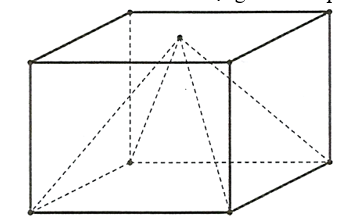
\includegraphics[scale=0.7]{images/Otc7Cau4TLN}
}
\loigiai{
Thể tích cái hộp là $V_1=30^3=27000$ (cm$^3$).\\
Xét đồ chơi có dạng hình chóp tứ giác đều, chiều cao của hình chóp bằng với một cạnh của hình lập phương, hay $h=30$ cm, đáy của hình chóp có diện tích $S=30^2=900$ cm$^2$.\\
Thể tích khối đồ chơi là
$V_2=\dfrac{1}{3}Sh=\dfrac{1}{3}\cdot 900\cdot 30=9000$ (cm$^3$).\\
Thể tích phần không gian bên trong chiếc hộp không bị chiếm bởi mô hình đồ chơi dạng hình chóp $V=V_1-V_2=27000-9000=18000$ (cm$^3$)$=18$ (dm$^3$).}
\end{ex}

\begin{ex}%[1H8V7-6]
Bạn An muốn làm các viên nước đá có dạng khối chóp cụt tứ giác đều có đáy lớn bằng $3 \mathrm{~cm}$, đáy nhỏ bằng $1,5 \mathrm{~cm}$ và cao $3 \mathrm{~cm}$ bằng cách dùng khay đá, mỗi khay sẽ tạo được $ 6 $ viên đá. Hỏi bạn An cần ít nhất bao nhiêu khay để chứa đồng thời $ 2 $ lít nước?
\shortans[0]{$22$}
\loigiai{
Ta có: $2 l=2000 \mathrm{~cm}^3$.\\
Thể tích: $V=\dfrac{1}{3} \cdot h \cdot\left(S+S'+\sqrt{S \cdot S'}\right)=\dfrac{1}{3} \cdot 3 \cdot\left(3^2+1,5^2+\sqrt{3^2 \cdot 1,5^2}\right)=\dfrac{63}{4} \mathrm{~cm}^3$.\\
Từ $ 2 $ lít nước có thể tạo ra số viên đá là: $\dfrac{2000}{\dfrac{63}{4}} \approx 127$ (viên).\\
Ta có: $127\colon 6 \approx 21,2$ (khay đá).\\
Vậy cần ít nhất $ 22 $ khay nước để chứa đồng thời $ 2 $ lít nước.
}
\end{ex}

\begin{ex}%[1H8V7-6]%[Dự án 2-Đúng Sai - CK2 NH23-24 - Mui Doan]
Bạn My muốn làm các viên nước đá có dạng khối chóp cụt tứ giác đều có đáy lớn bằng $3$ cm, đáy nhỏ bằng $1{,}5$ cm và cao $3$ cm bằng cách dùng khay đá, mỗi khay sẽ tạo được $6$ viên đá. Hỏi bạn An cần ít nhất bao nhiêu khay để chứa đồng thời $2$ lít nước?
\shortans[0]{$22$}
\loigiai{
Ta có $2\ell=2\,000$ cm$^3$.\\
Thể tích $V=\dfrac{1}{3}h\left(S+S'+\sqrt{SS'}\right)=\dfrac{1}{3}\cdot 3\cdot \left(3^2+1{,}5^2+\sqrt{3^2\cdot 1{,}5^2}\right)=\dfrac{63}{4}$ cm$^3$.\\
Từ $2$ lít nước có thể tạo ra số viên đá là $\dfrac{2\,000}{\dfrac{63}{4}}\approx 127$ (viên).\\
Ta có $127:6\approx 21{,}2$ (khay đá).\\
Vậy cần ít nhất $22$ khay nước để chứa đồng thời $2$ lít nước.
}
\end{ex}

\begin{ex}%[1H8V7-2]
Cho hình chóp $S\cdot ABC$ có đáy $ABC$ là tam giác đều cạnh $a$, $SA=9a$ và $SA\perp (ABC)$. Gọi $O$ là trọng tâm của tam giác $ABC$; $P$, $Q$ lần lượt là hai điểm thuộc cạnh $SB$ và $SC$ thỏa $\dfrac{SP}{SB}=\dfrac{SQ}{SC}=\dfrac{1}{3}$. Khi $a=\sqrt{3}$ thì thể tích khối tứ diện $AOPQ$ bằng bao nhiêu?
\shortans[0]{$1$}
\loigiai{
\begin{center}
\begin{tikzpicture}
\def\a{4} %Khai báo cạnh
\def\h{4}
\path 	(0:0) coordinate (A)
++(0:\a) coordinate (B)
++(-150:4*\a/5) coordinate (C)
($(A)+(90:\h)$) coordinate (S);
\coordinate (I) at ($(C)!0.5!(B)$);
\coordinate (O) at ($(A)!2/3!(I)$);
\coordinate (H) at ($(A)!2/3!(C)$);
\coordinate (P) at ($(S)!1/3!(C)$);
\coordinate (Q) at ($(S)!1/3!(B)$);
\draw[thick] 	(A)--(C)--(B)
(A)--(S)	(B)--(S)	(C)--(S) (H)--(P)--(Q) (A)--(P);
\draw[dashed,thick] 	(A)--(B) (A)--(I) (O)--(H) (Q)--(O) (A)--(Q) (O)--(P);
\foreach \x /\goc in {A/180,B/0,C/-135,S/90,I/-35,O/40,H/190,P/55,Q/50}
\fill[black] (\x) circle (1.5pt)
($(\x)+(\goc:3mm)$) node {$\x$};
\draw pic[draw,angle radius=2mm]{right angle=B--A--S};%Theo chiều dương
\end{tikzpicture}
\end{center}
Ta có $V_{S.ABC}=\dfrac{1}{3}\cdot SA\cdot S_{ABC}=\dfrac{1}{3}\cdot 9a\cdot \dfrac{\sqrt{3}}{4} a^2=\dfrac{3\sqrt{3}}{4} a^3$.\\
Kẻ $OH\parallel BC$, cắt $AB$ tại $H$.\\ Ta có $\dfrac{AH}{AB}=\dfrac{AO}{AI}=\dfrac{2}{3}$.
\[V_{O.APQ}=V_{H.APQ}=V_{Q.APH}=\dfrac{1}{3} d\left(Q,(SAB)\right)\cdot S_{\triangle APH}.\]
Mà $\dfrac{S_{\triangle APH}}{S_{\triangle ASB}}=\dfrac{d\left(P,AH\right)\cdot AH}{d\left(S,AB\right)\cdot AB}=\dfrac{2}{3}\cdot \dfrac{2}{3}=\dfrac{4}{9}$ và $\dfrac{d\left(Q,(SAB)\right)}{d\left(C,(SAB)\right)}=\dfrac{QA}{CA}=\dfrac{1}{3}$.\\
Suy ra $V_{Q.APH}=\dfrac{1}{3} d\left(Q,SAB\right)\cdot S_{\triangle APH}=\dfrac{4}{27}\cdot \dfrac{3\sqrt{3}}{4} a^3=\dfrac{\sqrt{3}}{9} a^3$.\\
Thay ${a=\sqrt{3}}$ nên $V_{Q.APH}=1$.
}
\end{ex}

\begin{ex}%[Ex-Ôn tập 2025, Hiếu Phan]%[1H8V7-9]
\immini{
Từ một tấm bìa mỏng hình vuông cạnh $6$ dm, bạn Hoa cắt bỏ bốn tam giác cân bằng nhau có cạnh đáy là cạnh của hình vuông ban đầu và đỉnh là đỉnh của một hình vuông nhỏ phía trong rồi gập lên, ghép lại tạo thành một khối chóp tứ giác đều như hình bên. Thể tích của khối chóp có giá trị lớn nhất bằng bao nhiêu decimét khối (làm tròn kết quả đến hàng phần mười)?
\shortans[]{$7{,}3$}
}
{\begin{tikzpicture}[scale=0.9, font=\footnotesize, line join=round, line cap=round, >=stealth]
\def\R{3} \def\r{0.45*\R}
\path (0,0) coordinate(O);
\foreach \i [count=\j from 0] in {B,A,D,C} \path ({90*\j+45}:\R) coordinate(\i);
\foreach \t [count=\k from 0] in {N,M,Q,P} \path ({90*\k}:\r) coordinate(\t);
\draw (A)--(B)node[midway, above]{$6$ dm}--(C)--(D)--cycle
(M)--(N)--(P)--(Q)--cycle
(A)--(M)--(B)--(N)--(C)--(P)--(D)--(Q)--(A);
\end{tikzpicture}}
\loigiai
{Giả sử miếng bìa là hình vuông $ABCD$, đáy của hình chóp tứ giác đều là hình vuông $MNPQ$ tâm $O$ có cạnh bằng $x$ dm ($0<x<6 \sqrt{2}$) như hình vẽ. Gọi $H$, $K$ lần lượt là trung điểm của $MQ$ và $NP$.
\begin{center}
\begin{tikzpicture}[scale=1, font=\footnotesize, line join=round, line cap=round, >=stealth]
\def\R{3} \def\r{0.45*\R}
\path (0,0) coordinate(O);
\foreach \i [count=\j from 0] in {B,A,D,C} \path ({90*\j+45}:\R) coordinate(\i);
\foreach \t [count=\k from 0] in {N,M,Q,P} \path ({90*\k}:\r) coordinate(\t);
\path ($(Q)!1/2!(M)$) coordinate(H)
($(P)!1/2!(N)$) coordinate(K);
\draw (A)--(B)node[midway, above]{$6$ dm} --(C)--(D)--cycle
(M)--(N)node[midway, sloped, above]{$x$ dm} --(P)--(Q)--cycle
(A)--(M)--(B)--(N)--(C)--(P)--(D)--(Q)--(A)
(A)--(C);
\foreach \p/\q in {A/135, B/45, C/-45, D/225, M/90, N/0, P/-90, Q/180, O/45, H/90, K/-90} {\fill (\p) node[shift={(\q:0.3)}]{$\p$} circle(1pt);}
\end{tikzpicture}
\hspace*{1cm}
\begin{tikzpicture}[scale=1, font=\footnotesize,line join=round, line cap=round, >=stealth]
\def\h{3}
\path (0,0) coordinate (N)
(-1.7,-1.2) coordinate (P)
++(4,0) coordinate (Q)
($(N)+(Q)-(P)$) coordinate(M)
($(M)!1/2!(P)$) coordinate(O)
++(0,\h) coordinate(A)
($(M)!1/2!(Q)$) coordinate(H)
($(N)!1/2!(P)$) coordinate(K);
\draw (A)--(P)--(Q)--(M)--(A)--(Q) (A)--(H);
\draw[dashed] (A)--(N)--(P) (N)--(M) (H)--(K) (A)--(O);
\foreach \diem/\pos in {A/90, N/160, P/-100, Q/-80, M/0, O/-90, K/-90, H/-70} \fill (\diem) node[shift={(\pos:0.3)}] {$\diem$} circle(1pt);
\path pic[draw,angle radius=0.2cm]{right angle=A--O--H};
\end{tikzpicture}
\end{center}
Vì $ABCD$ là hình vuông cạnh bằng $6$ dm nên $AC=6\sqrt{2}$ dm, $HK=x$ dm.\\
Ta có $AH=\dfrac{AC-HK}{2}=3\sqrt{2}-\dfrac{x}{2}$ dm.\\
Đường cao của hình chóp tứ giác đều là
\[h=AO=\sqrt{AH^2-OH^2}=\sqrt{\left(3\sqrt{2}-\dfrac{x}{2}\right)^2-\left(\dfrac{x}{2}\right)^2}=\sqrt{18-3\sqrt{2}x}.\]
Để tạo thành hình chóp thì đường cao $AO>0$, hay $x<3\sqrt{2}$.\\
Thể tích khối chóp là
\[V=\dfrac{1}{3}hx^2=\dfrac{1}{3}x^2\sqrt{18-3\sqrt{2}x}=\dfrac{1}{3}\sqrt{x^4\left(18-3\sqrt{2}x\right)}.\]
Để tìm giá trị lớn nhất của $V$ ta đi tìm giá trị lớn nhất của hàm số
\allowdisplaybreaks
\begin{eqnarray*}
f(x)=x^4\left(18-3\sqrt{2}x\right)\;\text{với}\;0<x<3\sqrt{2}.
\end{eqnarray*}
Ta có $f'(x)=x^3\left(-15 \sqrt{2} x+72\right)$, $f'(x)=0$ khi $x=0$ hoặc $x=\dfrac{12 \sqrt{2}}{5}$.\\
Bảng biến thiên của $f(x)$ như sau
\begin{center}
\begin{tikzpicture}[>=stealth,line join=round,line cap=round,font=\footnotesize,scale=1]
\tkzTabInit[nocadre=false,lgt=1.2,espcl=3.5,deltacl=.55]
{$x$/0.7, $f'(x)$/0.7, $f(x)$/2.5}
{$0$,$\dfrac{12\sqrt{2}}{5}$,$3\sqrt{2}$}
\tkzTabLine{$0$,+,0,-,}
\tkzTabVar{-/$0$,+/$f\left(\dfrac{12\sqrt{2}}{5}\right)$,-/$0$}
\end{tikzpicture}
\end{center}
Từ bảng biến thiên ta có $\max\limits_{(0; 3 \sqrt{2})}f(x)=f\left(\dfrac{12 \sqrt{2}}{5}\right)\approx 477{,}76$.\\
Vậy thể tích của khối chóp có giá trị lớn nhất bằng
\allowdisplaybreaks
\begin{eqnarray*}
V_{\max}\approx\dfrac{1}{3}\sqrt{477{,}76}\approx7{,}3\,\left(\text{dm}^3\right).
\end{eqnarray*}
}
\end{ex}

\begin{ex}%[1H8V7-9]%[Dự án toán Từ Tâm đợt 3]%[Nguyễn Ngọc Duy]
\immini{Một cái hộp hình lập phương, bên trong nó đựng một mô hình đồ chơi có dạng hình chóp tứ giác đều mà đỉnh của hình chóp đó trùng với tâm của một mặt chiếc hộp, giả sử hình vuông đáy của hình chóp trùng với một mặt của chiếc hộp (mặt này cùng với mặt chứa đỉnh hình chóp là hai mặt đối nhau). Biết cạnh của chiếc hộp bằng $30$ cm, thể tích phần không gian bên trong chiếc hộp không bị chiếm bởi mô hình đồ chơi dạng hình chóp (mô hình đồ chơi được làm bởi chất liệu nhựa đặc bên trong) đạt bao nhiêu dm$^3$?}
{\begin{tikzpicture}[declare function={r=2.5;},font = \footnotesize, line join=round, line cap=round, >=stealth, scale=1]
\path (0:0) coordinate (A)
(0:r) coordinate (B)
++(37:{0.65*r}) coordinate (C)
++(180:r) coordinate (D)
\foreach \x in {A,B,C,D}{(\x)++(90:r) coordinate (\x_1)};
\path ($(C_1)!0.5!(A_1)$) coordinate (E);
\draw[dashed] (D_1)--(D)--(A)--(E)--(D)--(C)--(E)--(B);
\draw (A)--(B)--(C) (A)--(A_1) (B)--(B_1) (C)--(C_1)(A_1)--(B_1)--(C_1)--(D_1)--cycle;
\fill (E) circle (1pt);
\end{tikzpicture}}
\par
\shortans{$18$}
\loigiai{
Thể tích cái hộp (khối lập phương) là $V_1=30^3=27\,000$ (cm$^3$).\\
Xét đồ chơi có dạng hình chóp tứ giác đều, chiều cao của hình chóp bằng với một cạnh của hình lập phương, hay $h=30$ cm, đáy của hình chóp có diện tích $S=30^2=900$ cm$^2$.\\
Thể tích khối đồ chơi (khối chóp tứ giác đều) là
\[V_2=\dfrac{1}{3} Sh=\dfrac{1}{3} \cdot 900\cdot 30=9\,000\, (\text{cm}^3).\]
Thể tích phần không gian bên trong chiếc hộp không bị chiếm bởi mô hình đồ chơi dạng hình chóp
\[V=V_1-V_2=27\,000-9\,000=18\,000\,(\text{cm}^3)=18\,(\text{dm}^3).\]
}
\end{ex}

\begin{ex}:%[1H8V7-9]
\immini{Một chiếc lồng đèn kéo quân có hình lăng trụ lục giác đều với cạnh đáy $8$ cm. Biết tổng diện tích các mặt bên của chiếc lồng đèn này bằng $1536$ cm$^2$. Tính thể tích của chiếc lồng đèn đó, kết quả làm tròn đến hàng đơn vị.}
{\begin{tikzpicture}[scale=0.7, font=\footnotesize, line join=round, line cap=round, >=stealth]
\path (0,0)coordinate (O)
($(O)+(10:2cm and 1cm)$)coordinate (A)
($(O)+(70:2cm and 1cm)$)coordinate (B)
($(O)+(130:2cm and 1cm)$)coordinate (C)
($(O)+(190:2cm and 1cm)$)coordinate (D)
($(O)+(-50:2cm and 1cm)$)coordinate (F)
($(O)+(-110:2cm and 1cm)$)coordinate (E)
($(A)+(0,4)$)coordinate (A')
($(B)+(0,4)$)coordinate (B')
($(C)+(0,4)$)coordinate (C')
($(D)+(0,4)$)coordinate (D')
($(E)+(0,4)$)coordinate (E')
($(F)+(0,4)$)coordinate (F')
;
\fill[color=blue!20](A)--(F)--(E)--(D)--(D')--(E')--(F')--(A')--(A);
\draw (A)--(A')(D)--(D')(E)--(E')(F)--(F');
\draw (D)--(E)--(F)--(A) (A')--(B')--(C')--(D')--(E')--(F')--(A');
\draw[dashed] (A)--(B)--(C)--(D)(B)--(B')(C)--(C');
\end{tikzpicture}}
\shortans{$5321 $}
\loigiai{
Gọi $h$ là chiều cao của chiếc lồng đèn. \\
Theo đề $6\cdot 8\cdot h=1536\Rightarrow h=32$ cm.\\
Diện tích mặt đáy của chiếc lồng đèn là $S=6\cdot \dfrac{8^2\sqrt{3}}{4}=96\sqrt{3}$ cm$^2$.\\
Thể tích của chiếc lồng đèn đó là $V=96\sqrt{3}\cdot 32\approx 5321$ cm$^3$.
}
\end{ex}

\begin{ex}%[1H8V7-9]
\immini
{
Cho một chậu nước hình chóp cụt đều (hình vẽ) có chiều cao bằng $3$ dm, đáy là lục giác đều, độ dài cạnh đáy lớn bằng $2$ dm và độ dài cạnh đáy nhỏ bằng $1$ dm. Tính thể tích của chậu nước (tính chính xác đến hàng phần mười của dm$^3$).
}
{
\begin{tikzpicture}[line join=round, line cap=round]
\def\a{2}
\def\b{3}
\draw[fill=cyan!50] (0:0) coordinate (A)  --++(0:\a)coordinate (B)--++(45:\a)coordinate (C)--++(135:\a)coordinate (D)--++(180:\a)coordinate (E)--++(225:\a)coordinate (F)--cycle;
\draw (-0.5,-3) coordinate (M) --++(0:\b)coordinate (N)--++(45:\b)coordinate (P)--++(135:\b)coordinate (Q)--++(180:\b)coordinate (K)--++(225:\b)coordinate (L)--cycle;
\draw[thick] (A)--(M) (B)--(N) (C)--(P) (D)--(Q) (E)--(K) (F)--(L);
\draw[pattern=horizontal lines light gray] (A)--(M)--(L)--(F)--cycle
(A)--(M)--(N)--(B)--cycle (B)--(C)--(P)--(N)--cycle
;
\draw[fill=cyan!50,opacity=.8] (0:0) coordinate (A)  --++(0:\a)coordinate (B)--++(45:\a)coordinate (C)--++(135:\a)coordinate (D)--++(180:\a)coordinate (E)--++(225:\a)coordinate (F)--cycle;
\end{tikzpicture}
}
\shortans{$18{,}2$}
\loigiai
{
Diện tích hai đáy của chậu bằng $S_1=6\left(\dfrac{2^2 \sqrt{3}}{4}\right)=6 \sqrt{3}$; $S_2=6\left(\dfrac{1^2 \sqrt{3}}{4}\right)=\dfrac{3 \sqrt{3}}{2}$.\\
Chiều cao của chậu bằng $h=3$.\\
Thể tích của chậu bằng
\[V=\frac{h}{3}\left(S_1+S_2+\sqrt{S_1 S_2}\right)=\dfrac{21\sqrt{3}}{2}\approx18{,}2 \ \left(\mathrm{dm}^3\right).\]
}
\end{ex}

\begin{ex}%[HSA-Lần 1, Đình Nguyên]%[1H8V7-4]
Cho hình lăng trụ đứng $ABC.A'B'C'$ có đáy $ABC$ là tam giác vuông tại $A$, $\widehat{ACB}=30^{\circ}$, biết góc giữa $B'C$ và mặt phẳng $(ACC'A')$ bằng $\alpha$ thỏa mãn $\sin\alpha = \dfrac{1}{2\sqrt{5}}$. Cho khoảng cách giữa hai đường thẳng $A'B$ và $CC'$ bằng $\sqrt{3}$. Thể tích $V$ của khối lăng trụ $ABC.A'B'C'$ bằng bao nhiêu? (Kết quả làm tròn đến hàng phần trăm)
\shortans{3,46}
\loigiai{
\immini{
Ta có $CC' \parallel AA' \Rightarrow CC' \parallel (AA'B'B)$.\\
Mà $A'B \subset (AA'B'B)$, nên
\[\mathrm{d}(CC', A'B) = \mathrm{d}(CC', (AA'B'B)) = C'A' = \sqrt{3}.\]
Xét $\triangle ABC$ vuông tại $A$ (do lăng trụ đứng nên $\triangle A'B'C'$ cũng vuông tại $A'$):
\begin{itemize}
\item $AC = A'C' = \sqrt{3}$.
\item $AB = A'B' = A'C' \cdot \tan 30^{\circ} = \sqrt{3} \cdot \dfrac{1}{\sqrt{3}} = 1$.
\end{itemize}
Suy ra diện tích đáy: $S_{ABC} = \dfrac{1}{2}AB \cdot AC = \dfrac{\sqrt{3}}{2}$.
}{
\begin{tikzpicture}[scale=1, font=\footnotesize, line join=round, line cap=round, >=stealth]
% Định nghĩa các điểm
\coordinate (A) at (0,3.5);
\coordinate (C) at (2.5,4.7);
\coordinate (B) at (-1.5,4.7);
\coordinate (A') at (0,0);
\coordinate (C') at (2.5,1.2);
\coordinate (B') at (-1.5,1.2);

% Vẽ các cạnh khuất
\draw[dashed] (C)--(B')--(C');

% Vẽ các cạnh thấy
\draw (A)--(C)--(B)--(A)--(A')--(C')--(C) (A')--(B)--(B')--(B)--(C) (B')--(A');

% Điểm
\foreach \p/\pos in {A/left, B/above, C/right, A'/left, B'/below, C'/right}
\fill[black] (\p) circle (1.5pt) node[\pos] {$\p$};
\end{tikzpicture}
}
Ta có $A'B' \perp A'C'$ (tam giác vuông) và $A'B' \perp AA'$ (lăng trụ đứng) nên $A'B' \perp (ACC'A')$.\\
Do đó, hình chiếu vuông góc của $B'$ lên mặt phẳng $(ACC'A')$ là điểm $A'$.\\
Góc giữa $B'C$ và mặt phẳng $(ACC'A')$ là góc $\widehat{B'CA'} = \alpha$.\\
Xét tam giác vuông $A'B'C$ (vuông tại $A'$ vì $A'B' \perp (ACC'A') \Rightarrow A'B' \perp A'C$):
\[ \sin\alpha = \dfrac{A'B'}{B'C} = \dfrac{1}{B'C} = \dfrac{1}{2\sqrt{5}} \Rightarrow B'C = 2\sqrt{5}. \]
Xét tam giác vuông $B'C'C$ (vuông tại $C'$):
\[ CC' = \sqrt{B'C^2 - B'C'^2} = \sqrt{(2\sqrt{5})^2 - (A'B'^2 + A'C'^2)}= \sqrt{20 - (1^2 + (\sqrt{3})^2)}=4. \]
Vậy thể tích khối lăng trụ là $ V = S_{ABC} \cdot CC' = \dfrac{\sqrt{3}}{2} \cdot 4 = 2\sqrt{3} \approx 3{,}46$.
}
\end{ex}

\begin{ex}%[Thái Văn Sang]%[MathTex_TN THPT 2026]%[1H8C7-9]
Cho một tấm bìa hình vuông có cạnh $2$ m. Từ tấm bìa này làm một mô hình kim tự tháp Ai Cập, người ta cắt bỏ bốn tam giác cân bằng nhau có cạnh đáy là các cạnh của hình vuông rồi gấp lên và ghép lại thành một hình chóp tứ giác đều. Thể tích của mô hình lớn nhất khi cạnh đáy của mô hình bằng $\dfrac{a\sqrt{2}}{b}$ m ($a$, $b \in \mathbb{Z}$; $a$, $b$ nguyên tố cùng nhau). Tính tổng $a^2+b^2$?
\shortans{$41$}
\loigiai{
\textbf{Phương pháp:}\\
Gọi độ dài cạnh đáy của hình chóp là $x$ (m). Tính thể tích theo $x$ và khảo sát hàm số tìm giá trị lớn nhất.\\
\textbf{Cách giải:}

\begin{center}
\begin{tikzpicture}[scale=0.6, font=\footnotesize, line join=round, line cap=round, >=stealth]
\path (0,0)coordinate(Q)
--++(-2,-2) coordinate(M)
--++(5,0) coordinate(N)
(Q)--+(5,0) coordinate (P)
(Q)--(N)coordinate[pos=0.5](O)
(O)--+(0,5) coordinate (S)
(M)--(N)coordinate[pos=0.5](K)
;
\draw (S)--(M)--(N)--(P)--cycle (S)--(N);
\draw[dashed] (O)--(S)--(Q) (Q)--(M) (Q)--(P) (Q)--(N) (M)--(P) (O)--(K);
\draw (S)--(K);
\draw pic[draw, angle radius=0.2cm]{right angle=S--O--N};
\draw pic[draw, angle radius=0.2cm]{right angle=O--K--N};
\foreach \p/\q in {Q/40,M/-90,N/-90,P/40,S/90,O/-90,K/-90}{
\path (\p) node[shift={(\q:3mm)}]{$\p$};
\fill[black] (\p) circle (1.2pt);}
\end{tikzpicture}
\end{center}
Gọi độ dài cạnh đáy của hình chóp là $x$ (m).\\
Do $MN < IJ = \sqrt{2} \Rightarrow x \in (0;\sqrt{2})$.\\
Ta có $OK = \dfrac{x}{2}; OA = \dfrac{AC}{2} = \sqrt{2} \Rightarrow SK = AK = \sqrt{2} - \dfrac{x}{2}$.\\
Do vậy: $SO = \sqrt{SK^2-OK^2} = \sqrt{\left(\sqrt{2}-\dfrac{x}{2}\right)^2 - \dfrac{x^2}{4}} = \sqrt{2-\sqrt{2}x}$.\\
Khi đó thể tích khối chóp là $V = \dfrac{1}{3}x^2\sqrt{2-\sqrt{2}x}$.\\
Xét $f(x) = \dfrac{1}{3}x^2\sqrt{2-\sqrt{2}x}$ với $x \in (0;\sqrt{2})$, ta có

\begin{eqnarray*}
f'(x) &=& \dfrac{1}{3}\left(2x\sqrt{2-\sqrt{2}x} - x^2 \dfrac{\sqrt{2}}{2\sqrt{2-\sqrt{2}x}}\right)\\
&=& \dfrac{1}{3}\left(\dfrac{4x(2-\sqrt{2}x) - \sqrt{2}x^2}{2\sqrt{2-\sqrt{2}x}}\right) = \dfrac{8x-5\sqrt{2}x^2}{6\sqrt{2-\sqrt{2}x}}.
\end{eqnarray*}
$f'(x) = 0 \Leftrightarrow 8x - 5\sqrt{2}x^2 = 0 \Leftrightarrow \left[ \begin{aligned} & x=0 \\ & x = \dfrac{4\sqrt{2}}{5} \end{aligned} \right.$.\\
Ta có bảng biến thiên:
\begin{center}
\begin{tikzpicture}
\tkzTabInit[lgt=1.2,espcl=3] % lgt: độ cao hàng, espcl: độ rộng cột
{$x$ /1, $f'(x)$ /1, $f(x)$ /2}
{$0$, $\dfrac{4\sqrt{2}}{5}$, $\sqrt{2}$}
\tkzTabLine{,+,0,-}
\tkzTabVar{-/ , +/ , -/ }
\end{tikzpicture}
\end{center}
Ta thấy thể tích của mô hình lớn nhất khi cạnh đáy của mô hình là \\
$x = \dfrac{4\sqrt{2}}{5} \Rightarrow a=4, b=5 \Rightarrow a^2+b^2 = 4^2+5^2 = 16+25 = 41$.
}
\end{ex}

\begin{ex}%[DuAnC-dot3, Đoàn Hùng]%[1H8C7-9]
Cho một tấm nhôm hình lục giác đều cạnh $90$ cm. Người ta cắt ở mỗi đỉnh của tấm nhôm hai hình tam giác vuông bằng nhau, biết cạnh góc vuông nhỏ bằng $x$ cm (cắt phần tô đậm của tấm nhôm) rồi gập tấm nhôm như hình vẽ để được một hình lăng trụ lục giác đều không có nắp. Tìm $x$ để thể tích của khối lăng trụ lục giác đều trên là lớn nhất. ({\it kết quả làm tròn đến hàng đơn vị})
\par\shortans[0]{15}
\begin{center}
\begin{tikzpicture}
\pgfmathsetmacro\n{6} % Số cạnh
\pgfmathsetmacro\r{2} % Bán kính
\pgfmathsetmacro{\goc}{360/\n}
\pgfmathsetmacro{\nn}{\n-1}
\path (0,0) coordinate (O);
\foreach \x in {0,...,\nn}
{
\pgfmathsetmacro{\xx}{int(\x+1)}
\path[fill=black] ($(O)+(\goc*\x:\r)$) coordinate (A\xx) circle (1pt)node[shift={(\goc*\x:9pt)}]{};
\path ($(O)!1/2!(A\xx)$) coordinate (a\xx);
\draw[rotate=\goc*\x] (0:\r)--(\goc:\r);
\draw (O)--(A\xx);
}
\path
(A6) coordinate (A0)
(A1) coordinate (A7)
;
\foreach \x in {1,...,\n}
{
\pgfmathsetmacro{\xx}{int(\x+1)}
\pgfmathsetmacro{\y}{int(\x-1)}
\path[fill=black]
($(A\x)!(a\x)!(A\y)$) coordinate (a\x\y) circle (1pt)
($(A\x)!(a\x)!(A\xx)$) coordinate (a\x\xx) circle (1pt)
;
\fill[pattern=north west lines]
(a\x)--(a\x\y)--(A\x)--(a\x\xx)--cycle;
\draw[rotate=\goc*\x] (0:\r/2)--(\goc:\r/2);
\draw (a\x\xx)--(a\x)--(a\x\y);
}
\path (current bounding box.south) node[below]{\bfseries Hình 1};
\end{tikzpicture}
\begin{tikzpicture}
\pgfmathsetmacro\n{6} % Số cạnh
\pgfmathsetmacro\r{2} % Bán kính
\pgfmathsetmacro{\goc}{360/\n}
\pgfmathsetmacro{\nn}{\n-1}
\path (0,0) coordinate (O);
\foreach \x in {0,...,\nn}
{
\pgfmathsetmacro{\xx}{int(\x+1)}
\path[fill=black] ($(O)+(\goc*\x:\r)$) coordinate (A\xx);
\path ($(O)!1/2!(A\xx)$) coordinate (a\xx);
%				\draw[rotate=\goc*\x] (0:\r)--(\goc:\r);
\draw (O)--(a\xx);
}
\path
(A6) coordinate (A0)
(A1) coordinate (A7)
;
\foreach \x in {1,...,\n}
{
\pgfmathsetmacro{\xx}{int(\x+1)}
\pgfmathsetmacro{\y}{int(\x-1)}
\path[fill=black]
($(A\x)!(a\x)!(A\y)$) coordinate (a\x\y)
($(A\x)!(a\x)!(A\xx)$) coordinate (a\x\xx)
;
%				\draw[rotate=\goc*\x](0:\r)--(\goc:\r);
%				\fill[white](a\x)--(a\x\y)--(A\x)--(a\x\xx)--cycle;
}
\path
(a1) coordinate (a7)
(a10) coordinate (a76)
;
\foreach \x in {1,...,\n}
{
\pgfmathsetmacro{\xx}{int(\x+1)}
\pgfmathsetmacro{\y}{int(\x-1)}
\draw[rotate=\goc*\x] (0:\r/2)--(\goc:\r/2);
\draw
(a\x\y)--(a\x)
(a\x\xx)--(a\x)
(a\x\xx)--(a\xx\x)
;
}
\path (current bounding box.south) node[below]{\bfseries Hình 2};
\end{tikzpicture}
\begin{tikzpicture}
\def\h{1.2}
\path
(0,0) coordinate (O)
+(180:1.5) coordinate (C)
++(150:1) coordinate (D)
+(0:1.3) coordinate (E)
($(O)!-1!(C)$) coordinate (F)
($(O)!-1!(D)$) coordinate (A)
($(O)!-1!(E)$) coordinate (B)
;
\foreach \p in {A,B,C,D,E,F}
\path ($(\p)+(90:\h)$) coordinate (\p');
\pgfresetboundingbox
\draw
(F)--(A)--(B)--(C)
(D')--(E')--(F')--(A')--(B')--(C')--cycle
;
\foreach \p/\q in {A/A',B/B',C/C',F/F'}
\draw (\p)--(\q)
;
\draw[dashed] (C)--(D)--(E)--(F) (D)--(D')
(E)--(E')
;
\path (current bounding box.south) node[below]{\bfseries Hình 3};
\end{tikzpicture}
\end{center}
\loigiai{
\begin{center}
\begin{tikzpicture}[font=\footnotesize]
\pgfmathsetmacro\n{6} % Số cạnh
\pgfmathsetmacro\r{2} % Bán kính
\pgfmathsetmacro{\goc}{360/\n}
\pgfmathsetmacro{\nn}{\n-1}
\path (0,0) coordinate (O);
\foreach \x in {0,...,\nn}
{
\pgfmathsetmacro{\xx}{int(\x+1)}
\path[fill=black] ($(O)+(\goc*\x:\r)$) coordinate (A\xx);
\path ($(O)!1/2!(A\xx)$) coordinate (a\xx);
%				\draw[rotate=\goc*\x] (0:\r)--(\goc:\r);
\draw (O)--(a\xx);
}
\path
(A6) coordinate (A0)
(A1) coordinate (A7)
;
\foreach \x in {1,...,\n}
{
\pgfmathsetmacro{\xx}{int(\x+1)}
\pgfmathsetmacro{\y}{int(\x-1)}
\path[fill=black]
($(A\x)!(a\x)!(A\y)$) coordinate (a\x\y)
($(A\x)!(a\x)!(A\xx)$) coordinate (a\x\xx)
;
%				\draw[rotate=\goc*\x](0:\r)--(\goc:\r);
%				\fill[white](a\x)--(a\x\y)--(A\x)--(a\x\xx)--cycle;
}
\path
(a1) coordinate (a7)
(a10) coordinate (a76)
;
\foreach \x in {1,...,\n}
{
\pgfmathsetmacro{\xx}{int(\x+1)}
\pgfmathsetmacro{\y}{int(\x-1)}
\draw[rotate=\goc*\x] (0:\r/2)--(\goc:\r/2);
\draw
(a\x\y)--(a\x)
(a\x\xx)--(a\x)
(a\x\xx)--(a\xx\x)
;
}
\path
(a5) node[below left]{$A$}
(a6) node[below right]{$B$}
(a56) node[below]{$H$}
(a65) node[below]{$K$}
;
\end{tikzpicture}
\end{center}
Điều kiện $0<x<45$.\\
Cạnh đáy của lăng trụ lục giác đều $AB=HK=90-2x$\\
Chiều cao của lăng trụ lục giác đều $HA=MH\cdot\tan 60^\circ=x\sqrt{3}$.\\
Diện tích đáy của lăng trụ lục giác đều $S_{ABCDEF}=6S_{ABO}=6\cdot\dfrac{\sqrt{3}}{4}{\left(90-2x\right)^2}$.\\
Thể tích của khối lăng trụ lục giác đều
\[V(x)=HA\cdot S_{ABCDEF}=\dfrac{9}{2}x{\left(90-2x\right)^2}\,\,
\text{hay}\,\, V(x)=18x^3-1620x^2+36450x.\]
Xét hàm số $V(x)=18x^3-1620x^2+36450x$ trên khoảng $\left(0;45\right)$.
\begin{align*}
V'(x)=& 54x^2-3240x+36450 =0\\
\Leftrightarrow &\, 54x^2-3240x+36450=0\\
\Leftrightarrow&\, \hoac{&x=15\\&x=45\ \text{(loại)}. }
\end{align*}
Bảng biến thiên
\begin{center}
\begin{tikzpicture}[>=stealth]
\tkzTabInit[nocadre=false,lgt=1.5,espcl=3,deltacl=1]{$x$/.7 ,$V'(x)$/.7,$V(x)$/2}
{$0$ , $15$ , $45$}
\tkzTabLine{ , + , $0$ , - , }
\tkzTabVar{-/$0$ , +/$243\,000$ , -/$0$}
\end{tikzpicture}
\end{center}
Từ bảng biến thiên ta có $\max\limits_{(0;45)}V(x)=243\,000$ (cm$^3$) khi và chỉ khi $x=15$ cm.\\
Vậy thể tích của khối lăng trụ lục giác đều lớn nhất khi và chỉ khi $x=15$ cm.
}
\end{ex}

\begin{ex}%[1H8C7-9]
Từ một tấm tôn hình vuông cạnh $16$ dm, bác Dũng cắt bỏ bốn phần như nhau ở bốn góc, sau đó bác hàn các mép lại để được một chiếc thùng (không có nắp) là một hình chóp cụt như hình vẽ. Hỏi thùng có thể chứa được nhiều nhất bao nhiêu lít? (Làm tròn kết quả đến hàng đơn vị).

\begin{center}
\begin{tikzpicture}[scale=0.5, font=\footnotesize, line join=round, line cap=round, >=stealth]
\path
(0,0) coordinate (E)
++ (0:8) coordinate (F)
++ (90:8) coordinate (G)
++ (180:8) coordinate (H)
(2,2) coordinate (A)
++ (0:4) coordinate (B)
++ (90:4) coordinate (C)
++ (180:4) coordinate (D)
(1,0) coordinate (A')
(7,0) coordinate (B')
(8,1) coordinate (J)
(8,7) coordinate (K)
(7,8) coordinate (C')
(1,8) coordinate (D')
(0,7) coordinate (L)
(0,1) coordinate (I)
(4,4) coordinate (O)
(9,0) coordinate (R)
(9,8) coordinate (Q)
;
\draw (A)--(B)--(C)--(D)--cycle;
\draw (E)--(F)--(G)--(H)--cycle;
\draw[dashed] (E)--(G) (F)--(H) (A)--(A') (A)--(I) (B)--(B') (B)--(J) (C)--(C') (C)--(K) (D)--(D') (D)--(L);
\draw[<->] (R)--(Q) node[sloped, pos=0.5, shift={(-90:3mm)}] {$16$ dm};
\draw (H)--(D') node[sloped, pos=0.5, shift={(90:3mm)}] {$2$ dm};
\draw (L)--(H) node[sloped, pos=0.5, shift={(90:3mm)}] {$2$ dm};
\draw (D)--(C) node[sloped, pos=0.5, shift={(90:3mm)}] {$8$ dm};
\foreach \i/\j in {O/-90, A/120, B/30, C/-30, D/-120, A'/-90, B'/-90, C'/90, D'/60, H/120, L/-150}{
\draw[fill=black] (\i) circle(0.5pt) node[shift={(\j:6mm)}] {$\i$};
}
\end{tikzpicture}

\begin{tikzpicture}[scale=0.5, font=\footnotesize, line join=round, line cap=round, >=stealth]
\path
(0,0) coordinate (E)
++ (0:8) coordinate (F)
++ (90:8) coordinate (G)
++ (180:8) coordinate (H)
(2,2) coordinate (A)
++ (0:4) coordinate (B)
++ (90:4) coordinate (C)
++ (180:4) coordinate (D)
(1,0) coordinate (A')
(7,0) coordinate (B')
(8,1) coordinate (J)
(8,7) coordinate (K)
(7,8) coordinate (C')
(1,8) coordinate (D')
(0,7) coordinate (L)
(0,1) coordinate (I)
(4,4) coordinate (O)
(9,0) coordinate (R)
(9,8) coordinate (Q)
;
\draw (A)--(B)--(C)--(D)--cycle;
\draw (A)--(A')--(B')--(B)-- (J)--(K)--(C)-- (C')--(D')--(D)-- (L)--(I)--(A);

\foreach \i/\j in {A/120, B/30, C/-30, D/-120, A'/-90, B'/-90, C'/90, D'/60, L/-150}{
\draw[fill=black] (\i) circle(0.5pt) node[shift={(\j:5mm)}] {$\i$};
}
\end{tikzpicture}
\begin{tikzpicture}[scale=0.5, font=\footnotesize, line join=round, line cap=round, >=stealth]
\path
(1,1) coordinate (A')
++ (0:6) coordinate (B')
++ (90:6) coordinate (C')
++ (180:6) coordinate (D')
(2,2) coordinate (A)
++ (0:4) coordinate (B)
++ (90:4) coordinate (C)
++ (180:4) coordinate (D)
;
\draw (A)--(B)--(C)--(D)--cycle;
\draw (A')--(B')--(C')--(D')--cycle;
\draw (A)--(A') (B)--(B') (C)--(C') (D)--(D');

\foreach \i/\j in {A/120, B/30, C/-30, D/-120, A'/-90, B'/-90, C'/90, D'/60}{
\draw[fill=black] (\i) circle(0.5pt) node[shift={(\j:3mm)}] {$\i$};
}
\end{tikzpicture}
\end{center}
\shortans{$351$}
\loigiai
{
\begin{center}
\begin{tikzpicture}[scale=0.7, font=\footnotesize, line join=round, line cap=round, >=stealth]
\path
(0,0) coordinate (E)
++ (0:8) coordinate (F)
++ (90:8) coordinate (G)
++ (180:8) coordinate (H)
(2,2) coordinate (A)
++ (0:4) coordinate (B)
++ (90:4) coordinate (C)
++ (180:4) coordinate (D)
(1,0) coordinate (A')
(7,0) coordinate (B')
(8,1) coordinate (J)
(8,7) coordinate (K)
(7,8) coordinate (C')
(1,8) coordinate (D')
(0,7) coordinate (L)
(0,1) coordinate (I)
(4,4) coordinate (O)
(9,0) coordinate (R)
(9,8) coordinate (Q)
(0.5,7.5) coordinate (M)
;
\draw (A)--(B)--(C)--(D)--cycle;
\draw (E)--(F)--(G)--(H)--cycle;
\draw[dashed] (E)--(G) (F)--(H) (A)--(A') (A)--(I) (B)--(B') (B)--(J) (C)--(C') (C)--(K) (D)--(D') (D)--(L)--(D');
\draw[<->] (R)--(Q) node[sloped, pos=0.5, shift={(-90:3mm)}] {$16$ dm};
\draw (H)--(D') node[sloped, pos=0.5, shift={(90:3mm)}] {$2$ dm};
\draw (L)--(H) node[sloped, pos=0.5, shift={(90:3mm)}] {$2$ dm};
\draw (D)--(C) node[sloped, pos=0.5, shift={(90:3mm)}] {$8$ dm};
\foreach \i/\j in {O/-90, A/120, B/30, C/-30, D/-120, A'/-90, B'/-90, C'/90, D'/60, H/120, L/-150, F/-30}{
\draw[fill=black] (\i) circle(0.5pt) node[shift={(\j:5mm)}] {$\i$};
}
\draw[fill=black] (M) circle(0.5pt) node[shift={(0:3mm)},font=\scriptsize] {$M$};
\pic[draw,angle eccentricity=1.8,angle radius=2mm]{right angle=L--M--D};
\end{tikzpicture}
\end{center}
Ta có $HM = MD' = \dfrac{2\sqrt{2}}{2} = \sqrt{2}$.\\
$HD = \dfrac{HF-DB}{2} = \dfrac{16\sqrt{2} - 8\sqrt{2}}{2} = 4\sqrt{2}$.\\
$\Rightarrow MD = HD - HM = 4\sqrt{2} - \sqrt{2} = 3\sqrt{2}$.\\
Áp dụng Định lí Pi-ta-go trong $\triangle D'MD$ vuông tại $M$.\\
$\Rightarrow D'D = \sqrt{D'M^2 + MD^2} = \sqrt{\sqrt{2}^2 + (3\sqrt{2})^2} = 2\sqrt{5}$.\\
Vì đây là hình chóp cụt đều nên \\
$CC' = DD' = AA' = BB' = 2\sqrt{5}$.\\
Lật ngược hình chóp cụt này lại.\\
\begin{center}
\begin{tikzpicture}[scale=1, font=\footnotesize, line join=round, line cap=round, >=stealth]
\path
(4,7) coordinate (S)
(0,0) coordinate (A')
(7,0) coordinate (B')
(8,3) coordinate (C')
(1,3) coordinate (D')
($(S)!1/3!(A')$) coordinate (A)
($(S)!1/3!(B')$) coordinate (B)
($(S)!1/3!(C')$) coordinate (C)
($(S)!1/3!(D')$) coordinate (D)
($(A)!1/2!(C)$) coordinate (O)
($(A')!1/2!(C')$) coordinate (O')
($(O')!1/3!(C')$) coordinate (E)

;
\draw (A)--(B)--(C)--(D)--cycle;
\draw (D')--(A')--(B')--(C') (A)--(C) (B)--(D);
\draw[dashed] (A')--(C')--(D')--(B') (O)--(O') (C)--(E);
\draw (A)--(A') (B)--(B') (C)--(C') (D)--(D');
\foreach \i/\j in {O/90, O'/-90, A/-170, B/-120, C/30, D/120, A'/-120, B'/-60, C'/0, D'/180, E/-90}{
\draw[fill=black] (\i) circle(0.5pt) node[shift={(\j:3mm)}] {$\i$};
}
\pic[draw,angle eccentricity=1.8,angle radius=2mm]{right angle=O--O'--C'};
\pic[draw,angle eccentricity=1.8,angle radius=2mm]{right angle=C--E--C'};
\draw (C)--(C') node[sloped, pos=0.5, shift={(90:3mm)}] {$2\sqrt{5}$ dm};

\end{tikzpicture}
\end{center}
Kẻ $CE \perp A'C'$ tại $E$. Khi đó $O'OCE$ là hình chữ nhật.\\
$\Rightarrow O'E = OC = \dfrac{AC}{2} = \dfrac{8\sqrt{2}}{2} = 4\sqrt{2}$.\\
Và $O'C = \dfrac{A'C'}{2} = \dfrac{A'B'\sqrt{2}}{2} = \dfrac{12\sqrt{2}}{2} = 6\sqrt{2}$.\\
$\Rightarrow EC'=O'C - O'E = 6\sqrt{2} - 4\sqrt{2} = 2\sqrt{2}$.\\
Áp dụng Định lí Pi-ta-go trong $\triangle CEC'$ vuông tại $E$.\\
$CE = \sqrt{CC'^2 - EC'^2} = \sqrt{(2\sqrt{5})^2 - (2\sqrt{2})^2} = 2\sqrt{3}$.\\
Đường cao của hình chóp cụt trên là \\
$OO' = CE = 2\sqrt{3}$.\\
Thể tích của hình chóp cụt là\\
\begin{align*}
V_{ABCD.A'B'C'D'} &= \dfrac{1}{3}(S_{ABCD} + S_{A'B'C'D'} + \sqrt{S_{ABCD}\cdot S_{A'B'C'D'}})\cdot OO' \\
&= \dfrac{1}{3}(8\cdot 8 + 12\cdot 12 + \sqrt{8\cdot 8 \cdot 12 \cdot 12})\cdot 2\sqrt{3} \\
&= \dfrac{608\sqrt{3}}{3}\\
&\approx 351.
\end{align*}
Vậy thể tích của thùng xấp xỉ là $351$ lít.
}
\end{ex}

\begin{ex}%[Dự án BG 10-11-LVH_Nguyễn Văn Hồng]%[1H8C7-9]
\immini{Giá đỡ ba chân đang được mở sao cho ba gốc chân cách đều nhau, góc giữa hai chân là $30^{\circ}$, các chân của giá đỡ dài $130$ $\mathrm{cm}$ (tham khảo hình vẽ). Chiều cao của giá đỡ là bao nhiêu $\mathrm{cm}$? (làm tròn đến hàng đơn vị).}
{
\definecolor{battleshipgrey}{rgb}{0.8, 0.8, 0.8}
\definecolor{mau2}{rgb}{0.52, 0.52, 0.51}
\definecolor{arsenic}{rgb}{0.23, 0.27, 0.29}
\begin{tikzpicture}[scale=1,>=stealth, font=\footnotesize, line join=round, line cap=round,declare function={h=5;k=0.05;r=0.3;}]
\path
(0,0) coordinate (C)
(1,-1) coordinate (B)
(5,-0.3) coordinate (A)
(barycentric cs:A=1,C=1,B=1)coordinate(H)
(H)+(90:h) coordinate (T)
($(T)!k!(A)$) coordinate (D)
($(T)!k!(B)$) coordinate (E)
($(T)!k!(C)$) coordinate (F)
($(T)!k!(H)$) coordinate (S)
(S)+(r,0) coordinate (l)
\foreach \i/\t/\p in{A/At/Ap,B/Bt/Bp,C/Ct/Cp,D/Dt/Dp,E/Et/Ep,F/Ft/Fp}{
($(\i)+(-0.07,0)$) coordinate (\t)
($(\i)+(0.07,0)$) coordinate (\p)
}
(intersection of At--Dt and Bp--Ep) coordinate (T')

;
\foreach \x/\y/\u/\v in{At/Ap/Dp/Dt,Ct/Cp/Fp/Ft,Bt/Bp/Ep/Et}{
\draw [fill=battleshipgrey](\x)--(\y)--(\u)--(\v)--cycle;
}
;
\draw[fill=mau2] (l) arc (0:360:r-0.01 and 0.45*r);
%			\draw[dashed] (S)--(H)--(A);
\draw (A)--(B)node[midway,sloped,pos=0.5,scale=0.6]{$||$};
\draw (A)--(C)node[midway,sloped,pos=0.5,scale=0.6]{$||$};
\draw (B)--(C)node[midway,sloped,pos=0.5,scale=0.6]{$||$};
\draw[fill=arsenic] ($(A)+(0.15,-0.05)$)-++(-0.08,0.1)-++(-0.3,0.15)-++(-0.4,0)--cycle;
\draw[fill=arsenic] ($(C)+(-0.15,-0.05)$)-++(0.08,0.1)-++(0.3,0.15)-++(0.4,0)--cycle;
\draw[fill=arsenic] ($(B)+(-0.03,-0.05)$)-++(0.05,0.1)-++(0.1,0.15)-++(0.2,0.1)--cycle;
\draw[fill=arsenic] ($(B)+(-0.15,-0.02)$)-++(0.05,0.1)-++(0.08,0.12)-++(0.07,0.05)--cycle;
\draw[fill=arsenic] ($(B)+(-0.03,-0.05)$)-++(-0.12,0.03)-++(-0.08,0.04)-++(0,0.02)--cycle;
\pic[draw,angle radius=20]{angle=Bp--T'--At};
\path (T') node[shift={(-75:1)},scale=1]{$30^{\circ}$};
%			\pic[draw,angle radius=5]{right angle=S--H--A};
\path($(A)!0.5!(D)$) node[shift={(30:.6)},scale=1]{$130~\mathrm{cm}$};
%			\foreach \p/\g in{A/-90,B/-90,C/-100,S/90,H/-120}
%			\shade[shading=ball](\p)circle(.03)node[shift={(\g:.3)},scale=1]{$\p$};
\end{tikzpicture}
}
\shortans{$124$}
\loigiai{
\begin{center}
\definecolor{battleshipgrey}{rgb}{0.8, 0.8, 0.8}
\definecolor{mau2}{rgb}{0.52, 0.52, 0.51}
\definecolor{arsenic}{rgb}{0.23, 0.27, 0.29}
\begin{tikzpicture}[scale=1,>=stealth, font=\footnotesize, line join=round, line cap=round,declare function={h=5;k=0.05;r=0.3;}]
\path
(0,0) coordinate (C)
(1,-1) coordinate (B)
(5,-0.3) coordinate (A)
(barycentric cs:A=1,C=1,B=1)coordinate(H)
(H)+(90:h) coordinate (T)
($(T)!k!(A)$) coordinate (D)
($(T)!k!(B)$) coordinate (E)
($(T)!k!(C)$) coordinate (F)
($(T)!k!(H)$) coordinate (S)
(S)+(r,0) coordinate (l)
\foreach \i/\t/\p in{A/At/Ap,B/Bt/Bp,C/Ct/Cp,D/Dt/Dp,E/Et/Ep,F/Ft/Fp}{
($(\i)+(-0.07,0)$) coordinate (\t)
($(\i)+(0.07,0)$) coordinate (\p)
}
(intersection of At--Dt and Bp--Ep) coordinate (T')

;
\foreach \x/\y/\u/\v in{At/Ap/Dp/Dt,Ct/Cp/Fp/Ft,Bt/Bp/Ep/Et}{
\draw [fill=battleshipgrey](\x)--(\y)--(\u)--(\v)--cycle;
}
;
\draw[fill=mau2] (l) arc (0:360:r-0.01 and 0.45*r);
\draw[dashed] (S)--(H)--(A);
\draw (A)--(B)node[midway,sloped,pos=0.5,scale=0.6]{$||$};
\draw (A)--(C)node[midway,sloped,pos=0.5,scale=0.6]{$||$};
\draw (B)--(C)node[midway,sloped,pos=0.5,scale=0.6]{$||$};
\draw[fill=arsenic] ($(A)+(0.15,-0.05)$)-++(-0.08,0.1)-++(-0.3,0.15)-++(-0.4,0)--cycle;
\draw[fill=arsenic] ($(C)+(-0.15,-0.05)$)-++(0.08,0.1)-++(0.3,0.15)-++(0.4,0)--cycle;
\draw[fill=arsenic] ($(B)+(-0.03,-0.05)$)-++(0.05,0.1)-++(0.1,0.15)-++(0.2,0.1)--cycle;
\draw[fill=arsenic] ($(B)+(-0.15,-0.02)$)-++(0.05,0.1)-++(0.08,0.12)-++(0.07,0.05)--cycle;
\draw[fill=arsenic] ($(B)+(-0.03,-0.05)$)-++(-0.12,0.03)-++(-0.08,0.04)-++(0,0.02)--cycle;
\pic[draw,angle radius=20]{angle=Bp--T'--At};
\path (T') node[shift={(-75:1)},scale=1]{$30^{\circ}$};
\pic[draw,angle radius=5]{right angle=S--H--A};
\path($(A)!0.5!(D)$) node[shift={(30:.6)},scale=1]{$130~\mathrm{cm}$};
\foreach \p/\g in{A/-90,B/-90,C/-100,S/90,H/-120}
\shade[shading=ball](\p)circle(.03)node[shift={(\g:.3)},scale=1]{$\p$};
\end{tikzpicture}
\end{center}
Xét $\triangle SAB$ là tam giác cân tại $S$. Khi đó, $\widehat{SBA}=\dfrac{180^{\circ} -30^{\circ}}{2}=75^{\circ}$.\\
Áp dụng định lí sin ta có\\
$\dfrac{AB}{\sin\widehat{BSA}}=\dfrac{SA}{\sin\widehat{SBA}}$ $\Leftrightarrow$ $\dfrac{AB}{\sin 30^{\circ}}=\dfrac{SA}{\sin 75^{\circ}}$ $\Leftrightarrow$ $AB=\dfrac{SA\cdot \sin 30^{\circ}}{\sin 75^{\circ}}\approx 67{,}29$ $\mathrm{cm}$.\\
Nhận xét rằng $H$ là trọng tâm tam giác đều $ABC$.\\
$AH=\dfrac{2}{3}\dfrac{AB\sqrt{3}}{2}=\dfrac{AB\sqrt{3}}{3}$ $\mathrm{cm}$.\\
$SH=\sqrt{SA^2-AH^2}\approx\sqrt{130^2-\dfrac{(67{,}29)^2}{3}}\approx 124$ $\mathrm{cm}$.
}
\end{ex}

\begin{ex}%[Dự án BG 10-11-LVH_Nguyễn Văn Hồng]%[1H8C7-9]
\immini[thm]{Một công ty sản xuất một chiếc gối dành cho người bị bệnh trào ngược dạ dày có hình dạng là một khối lăng trụ tam giác có kích thước như hình vẽ. Khối lăng trụ có thể tích bằng bao nhiêu dm$^3$ (làm tròn kết quả điến hàng phần chục của dm$^3$)?}
{\begin{tikzpicture}[>=stealth,line join=round,line cap=round,font=\footnotesize,scale=0.65]
\path (0,0) coordinate (O)
(0,2) coordinate (A)
(-3,-2) coordinate (o)
(4,0) coordinate (B)
($(A)+(o)-(O)$) coordinate (a)
($(B)+(o)-(O)$) coordinate (b)
;
\draw (A)--(a)--(o)--(b)--(B)--(A) (a)--(b);
\draw[dashed] (A)--(O)--(o) (O)--(B);
\foreach \p in {O,A,B,o,a,b}
\fill (\p) circle (1.2pt);
\node at (-1,-2.5) {$65$ cm};
\node at (3.2,-1.5) {$60$ cm};
\node at (-3.8,-1) {$16$ cm};
\pic[draw,angle radius=2mm,angle eccentricity=1.5] {right angle = a--o--b};
\end{tikzpicture}}
\shortans{$31{,}2$}
\loigiai{Diên tích đáy của khối lăng trụ là $S=\dfrac{1}{2}\cdot1{,}6\cdot6{,}5=5{,}2$ dm$^2$.\\
Thể tích của gối là $V=5{,}2\cdot6=31{,}2$ dm$^3$.}
\end{ex}

\begin{ex}%[Dự án BG 10-11-LVH_Nguyễn Văn Hồng]%[1H8C7-9]
Cho một tấm nhôm hình vuông có cạnh $1$ m như hình vẽ dưới đây. Người ta cắt phần tô đậm của tấm nhôm rồi gập thành hình chóp tứ giác đều có cạnh đáy bằng $\dfrac{\sqrt{2}}{3}$\,(m). Khoảng cách từ đỉnh $ S$ tới đáy $\left(ABCD\right)$ bằng $\dfrac{a\sqrt{6}}{b}$ (m), với $ a,\,b$ là các số nguyên dương và phân số $\dfrac{a}{b}$ tối giảng. Tính giá trị của $b^2-a^2$?
\begin{center}
\begin{tikzpicture}[line join=round, line cap=round,thick]
\coordinate (E) at (1,5);
\coordinate (F) at (1,1);
\coordinate (G) at (5,5);
\coordinate (K) at ($(G)-(E)+(F)$);
\coordinate (A) at (2,3);
\coordinate (B) at (3,2);
\coordinate (C) at (4,3);
\coordinate (D) at (3,4);
\draw(E)--(F)--(K)--(G)--cycle;
\fill[pattern=north east lines](E)--(F)--(A)--cycle;
\fill[pattern=north east lines](F)--(K)--(B)--cycle;
\fill[pattern=north east lines](K)--(G)--(C)--cycle;
\fill[pattern=north east lines](G)--(E)--(D)--cycle;
\draw (E)--(D)--(G)--(C)--(C)--(K)--(B)--(F)--(A)--(E)  (A)--(B)--(C)--(D)--(A);
\end{tikzpicture}
\begin{tikzpicture}[line join=round,line cap=round,line width=.6pt,font=\footnotesize,scale=1]
\coordinate (B) at (0,0);
\coordinate (A) at (1,1);
\coordinate (C) at (4,0);
\coordinate (D) at ($(C)-(B)+(A)$);
\coordinate(O) at ($(A)!.5!(C)$);
\coordinate (S) at ($(O)+(90:4)$);
\draw (B)--(C)--(D)--(S)--cycle (S)--(C);
\draw[dashed] (C)--(A)--(D)--(B) (O)--(S)--(A)--(B) (S);


\foreach \i/\g in {	A/40,  B/-150, C/-20, D/10,  O/-80, S/90	}
\fill (\i) circle (1pt)+(\g:3mm) node {$\i$};
\end{tikzpicture}
\end{center}
\shortans{35}
\loigiai{
\begin{center}
\begin{tikzpicture}[line join=round, line cap=round,thick]
\coordinate (E) at (1,5);
\coordinate (F) at (1,1);
\coordinate (G) at (5,5);
\coordinate (K) at ($(G)-(E)+(F)$);
\coordinate (A) at (2,3);
\coordinate (B) at (3,2);
\coordinate (C) at (4,3);
\coordinate (D) at (3,4);
\draw(E)--(F)--(K)--(G)--cycle;
\draw (F) node[left]{$S'$};
\draw (G) node[right]{$S$};
\coordinate (L) at (intersection of A--B and G--F);
\coordinate (H) at (intersection of C--D and G--F);
\draw (E)--(D)--(G)--(C)--(C)--(K)--(B)--(F)--(A)--(E)  (A)--(B)--(C)--(D)--(A)--(C)  (B)--(D)  (F)--(G)  (E)--(K);
\foreach \i/\g in {H/0,L/0,A/180,B/-90,C/0,D/90}{\draw[fill=white](\i) circle (1.5pt) ($(\i)+(\g:3mm)$) node[scale=1]{$\i$};}
\end{tikzpicture}
\begin{tikzpicture}[line join=round,line cap=round,line width=.6pt,font=\footnotesize,scale=1]
\coordinate (B) at (0,0);
\coordinate (A) at (1,1);
\coordinate (C) at (4,0);
\coordinate (D) at ($(C)-(B)+(A)$);
\coordinate (O) at ($(A)!.5!(C)$);
\coordinate (S) at ($(O)+(90:4)$);
\coordinate (H) at ($(C)!0.5!(D)$);
\draw (B)--(C)--(D)--(S)--cycle (S)--(C)  (H)--(S);
\draw[dashed] (C)--(A)--(D)--(B) (O)--(S)--(A)--(B)  (O)--(H);


\foreach \i/\g in {	A/40,  B/-150, C/-20, D/10,  O/-80, S/90, H/0	}
\fill (\i) circle (1pt)+(\g:3mm) node {$\i$};
\end{tikzpicture}
\end{center}
Khi gập tấm nhôm ta thấy $S\equiv{S}'$.\\
Dễ thấy $S'L=LH=HS=\dfrac{\sqrt{2}}{3}$; $ OH=\dfrac{1}{2}HL=\dfrac{\sqrt{2}}{6}$, $SO=\sqrt{S{H^2}-O{H^2}}=\dfrac{\sqrt{6}}{6}$ (m).\\
Với $ a=1,\,b=6$ thì $b^2-a^2$ đạt giá trị bằng $35$.}
\end{ex}

\begin{ex}%[24 - 24 giảng K10 - K11, Dat Tien Pham]%[1H8C7-9]
Người ta muốn xây một bể bơi hình hộp chữ nhật có thể tích là $125$ m$^3$. Đáy bể bơi là hình chữ nhật có chiều dài gấp ba lần chiều rộng. Tính chiều rộng của đáy bể bơi để khi thi công tiết kiệm được nguyên liệu nhất (làm tròn đến hai chữ số thập phân).
\shortans{$3,82$}
\loigiai{
\begin{itemize}
\item Gọi chiều rộng đáy là $a$, chiều rộng là $b$, chiều dài là $3a$. Theo bài ra ta có $3a^2\cdot b =125\Rightarrow b=\dfrac{125}{3a^2}$.
\item Diện tích toàn phần: $2(3a+a)\cdot b+a\cdot 3a=8a\cdot \dfrac{125}{3a^2}+3a^2=\dfrac{125\cdot 8}{3a}+3a^2$ (chỉ có 1 mặt đáy).
\item Ta có: $\dfrac{125\cdot 8}{3a}+3a^2=\dfrac{125\cdot 4}{3a}+\dfrac{125\cdot 4}{3a}+3a^2\ge 3 \sqrt[3]{\dfrac{125\cdot 4}{3a}\cdot \dfrac{125\cdot 4}{3a}\cdot 3a^2}=10\sqrt[3]{12}$.\\ Dấu \lq\lq$=$\rq\rq \ xảy ra khi: $\dfrac{125\cdot 4}{3a}=3a^2\Rightarrow a=5\cdot \sqrt[3]{\dfrac{4}{9}}\approx 3,82$.
\end{itemize}
}
\end{ex}

\begin{ex}%[24 - 24 giảng K10 - K11, Dat Tien Pham]%[1H8C7-9]
\immini
{
Bể cá hai ngăn không có nắp phía trên thể tích là $1{,}296$ cm$^3$ bằng cách cắt các tấm kính thành hình hộp chữ nhật có các kích thước $a$, $b$, $c$ (xem hình vẽ). Tính $a+b+c$ để tiết kiệm chi phí nhất.
\shortans{$3,6$}
}
{\vspace*{-0.5cm}
\begin{tikzpicture}[scale=0.5, font=\footnotesize, line join=round, line cap=round, >=stealth]
\path
(5,-3)coordinate(A)
(8,-2)coordinate(B)
(7,-4)coordinate(D)
(11,-1)coordinate(C)
(10,-3)coordinate(E)
(13,-2)coordinate(F)
(8,3)coordinate(G)
(5,2)coordinate(H)
(7,1)coordinate(I)
(10,2)coordinate(J)
(11,4)coordinate(K)
(13,3)coordinate(L)
(5.9,-3.2)coordinate(O)node[right]{$b$}
(11,-2.2)coordinate(P)node[right]{$a$}
(12.2,0.58)coordinate(Q)node[right]{$c$}
;
\draw
(A)--(D)--(F)--(L)--(K)--(H)--(I)--(L)(G)--(J)
(D)--(I)(A)--(H)(E)--(J)
;
\draw[dashed]
(A)--(C)--(K)(B)--(G)(B)--(E)(C)--(F)
;
\end{tikzpicture}
}
\loigiai
{
Thể tích bể cá là $V=abc=1{,}296$.\\
Diện tích tổng các miếng kính là $S=ab+2ac+3bc$ (kể cả miếng ở giữa).\\
Ta có $\dfrac{S}{abc}=\dfrac{1}{c}+\dfrac{2}{b}+\dfrac{3}{a}\geqslant3\sqrt[3]{\dfrac{1}{c}\cdot\dfrac{2}{b}\cdot{3}{a}}=\dfrac{3\sqrt[3]{6}}{\sqrt{abc}}=\dfrac{3\sqrt[3]{6}}{1{,}296}$.\\
Dấu \lq\lq$=$\rq\rq\ xảy ra khi $\heva{ & \dfrac{1}{c}=\dfrac{2}{b}=\dfrac{3}{a}\\ & abc=1{,}296}\Leftrightarrow \heva{ & a=1{,}8\\ & b=1{,}2\\ & c=0{,}6}$.
}
\end{ex}

\begin{ex}%[1H8C7-9]%[tex hóa đề ck2 - form 2025 - đợt 2 - Hồ Văn Trung]
Một tấm kẽm hình vuông $ABCD$ có cạnh bằng $30$ cm. Người ta gập tấm kẽm theo hai cạnh $EF$ và $GH$ cho đến khi $AD$ và $BC$ trùng nhau như hình vẽ bên để được một hình lăng trụ khuyết hai đáy. Khi thể tích khối lăng trụ lớn nhất thì khoảng cách từ $A$ đến mặt phẳng $(EFGH)$ bằng $a\sqrt{b}$ (cm) với $a,b$ là các số nguyên dương. Tính $T=a+2024b$.
\begin{center}
\begin{tikzpicture}[smooth,samples=300,scale=0.8,y=0.8cm,>=stealth,font=\footnotesize]
\draw (0,0)--(0,4) (1,4)--(1,0) (2.5,0)--(2.5,4) (3.5,0)--(3.5,4) (0,0)--(3.5,0) (0,4)--(3.5,4) (5,0)--(5,4)--(6.5,4)--(6.5,0)--(5.8,-0.5)--(5,0) (5,4)--(5.8,3.5)--(6.5,4) (5.8,-0.5)--(5.8,3.5);
\draw[dashed] (5,0)--(6.5,0);
\path[] (0,0) node[below]{$D$} (1,0) node[below]{$F$} (5,0) node[left]{$D$} (2.5,0) node[below]{$H$} (3.5,0) node[below]{$C$} (0,4) node[above]{$A$} (1,4) node[above]{$E$} (2.5,4) node[above]{$G$} (3.5,4) node[above]{$B$} (5,4) node[above]{$E$} (6.5,4) node[above]{$G$} (6.5,0) node[right]{$C$} (5.8,-0.5) node[left]{$F$} node[right]{$H$} (5.8,3.5) node[left]{$A$} node[right]{$B$} (0.5,0) node[below]{$x$} (3,0) node[below]{$x$};
\end{tikzpicture}
\end{center}
\shortans[0]{$6077$}
\loigiai{
Thể tích khối lăng trụ là $V=BC \cdot S_{\triangle AEG}=30S_{\triangle AEG}$. Theo giả thiết ta có $2x<30 \Leftrightarrow x<15$.\\
Ta có $\triangle AEG$ có độ dài các cạnh là $AE=AG=x$ (cm), $EG=30-2x$ (cm) nên diện tích là
\begin{center}
$S=\sqrt{15(15-x)(15-x)[15-(30-2x)]}=\sqrt{15(15-x)(15-x)(2x-15)}$ (cm$^2$).
\end{center}
Áp dụng bất đẳng thức Cô-si cho ba số $\sqrt{15-x},\;\sqrt{15-x},\;\sqrt{2x-15}$ ta được
\begin{center}
$\sqrt{(15-x)(15-x)(2x-15)} \leq \sqrt{\left(\dfrac{(15-x)+(15-x)+(2x-15)}{3} \right) }=\sqrt{5^3}$
\end{center}
Giá trị lớn nhất của thể tích đạt được khi và chỉ khi diện tích $S_{\triangle AEG}$ đạt giá trị lớn nhất khi đó $\heva{&15-x=2x-15\\&0<x<15} \Leftrightarrow x=10$.\\
Vì $x=10$ nên tam giác $AEG$ đều do đó $\mathrm{d}(A,EG)=\dfrac{10\sqrt{3}}{2}=5\sqrt{3}$.\\
Do $(AEG)$ vuông góc với $(EFGH)$ nên khoảng cách từ $A$ đến $(EFGH)$ bằng độ dài đường cao kẻ từ $A$ đến $EG$.\\
Vậy $\mathrm{d}(A,(EFGH))=5\sqrt{3}$ (cm) $\Rightarrow \heva{&a=5\\&b=3} \Rightarrow T=a+2024b=5+2024 \cdot 3=6077$.
}
\end{ex}

\begin{ex}%[1H8C7-7]
Cho hình chóp $S.ABCD$ có đáy là hình thoi tâm $O$ cạnh $a$, $\widehat{BAD} = 135^\circ$. Biết $SA = 2a$ và tạo với mặt phẳng đáy một góc $60^\circ$. Gọi $I$ là trung điểm của $SO$, $(P)$ là mặt phẳng đi qua $BI$ và song song với cạnh $AC$, $(P)$ chia hình chóp $S.ABCD$ thành hai phần. Biết thể tích của phần nhỏ hơn là $\dfrac{a^3\sqrt{n}}{m}$, với $m, n \in \mathbb{N}^*$; $m+n < 60$. Tính giá trị của biểu thức $T = \dfrac{m}{n^2}$.
\shortans{$1$}
\loigiai{
\begin{center}
\begin{tikzpicture}[line join=round, line cap=round, >=stealth, font=\footnotesize, scale=1]
\path
(0,0) coordinate (A)
(-2,-3) coordinate (B)
(4,-3) coordinate (C)
(6,0) coordinate (D)
(0.5,4.5) coordinate (S)
($(A)!1/2!(C)$) coordinate (O)
($(S)!1/2!(O)$) coordinate (I)
($(B)!1.5!(I)$) coordinate (X)
(intersection of B--X and S--D) coordinate (P)
($(B)!1.5!(I)$) coordinate (X)
($(I)+(C)-(O)$) coordinate (Y)
(intersection of I--Y and S--C) coordinate (N)
($(I)+(A)-(O)$) coordinate (Z)
(intersection of I--Z and S--A) coordinate (M)
($(P)!1/2!(D)$) coordinate (K)
;
\draw (B)--(C) (C)--(D) (S)--(B) (S)--(D) (S)--(C) (B)--(N) (P)--(N);
\draw[dashed] (A)--(B) (A)--(D) (A)--(S) (A)--(C) (B)--(D) (S)--(O) (B)--(I) (M)--(N) (M)--(P) (M)--(B) (I)--(P) (O)--(K);
\foreach \i/\j in {A/180, B/-90, C/-90, D/0, S/90, M/180, N/0, O/-90, I/180, P/0, K/45} \fill (\i) node[shift={(\j:0.3)}]{$\i$} circle(1pt);
\end{tikzpicture}
\end{center}
Mặt phẳng $(P)$ cắt $SA$, $SC$, $SD$ lần lượt tại $M$, $N$, $P$.\\
Do $(P) \parallel AC \Rightarrow MN \parallel AC$ mà $I$ là trung điểm của $SO$ nên $M$, $N$ lần lượt là trung điểm của $SA$, $SC$.\\
Gọi $K$ là trung điểm $PD$.\\
Xét tam giác $BPD$ có $O, K$ lần lượt là trung điểm $DB, DP$ nên $OK \parallel BP$.\\
Xét tam giác $SOK$ có $I$ là trung điểm $SO$, mà $IP \parallel OK$ nên $P$ là trung điểm $SK \Rightarrow SP = PK = KO$.\\
Có
$\heva{&\dfrac{V_{S.PBN}}{V_{S.DBC}} = \dfrac{SN}{SC} \cdot \dfrac{SP}{SD} = \dfrac{1}{2} \cdot \dfrac{1}{3} = \dfrac{1}{6}\\&\dfrac{V_{S.PBM}}{V_{S.DBA}} = \dfrac{SM}{SA} \cdot \dfrac{SP}{SD} = \dfrac{1}{2} \cdot \dfrac{1}{3} = \dfrac{1}{6}} \Rightarrow \dfrac{V_{S.BNPM}}{V_{S.ABCD}} = \dfrac{1}{6}$.\\
Chiều cao của hình chóp $h = SA \cdot \cos (\widehat{SA, (ABCD)}) = 2a \cdot \cos 60^\circ = a$.\\
$\Rightarrow V_{S.ABCD} = \dfrac{1}{3} S_{ABCD} \cdot h = \dfrac{1}{3} \cdot a \cdot a \cdot \sin 135^\circ \cdot a\sqrt{3} = \dfrac{a^3\sqrt{6}}{6}$.\\
$\Rightarrow V_{SBNPM} = \dfrac{1}{6} V_{S.ABCD} = \dfrac{1}{6} \cdot \dfrac{a^3\sqrt{6}}{6} = \dfrac{a^3\sqrt{6}}{36}$.\\
Từ đó $n=6$, $m=36$.\\
Suy ra $m+n = 36+6 = 42 < 60$.\\
Do đó, giá trị của biểu thức $T = \dfrac{m}{n^2} = \dfrac{36}{6^2} = 1$.
}
\end{ex}

\begin{ex}%[1H8C7-7]
Cho hình chóp $S.ABCD$ có đáy là hình thoi tâm $O$ cạnh $a$, $\widehat{BAD} = 135^\circ$. Biết $SA = 2a$ và tạo với mặt phẳng đáy một góc $60^\circ$. Gọi $I$ là trung điểm của $SO$, $(P)$ là mặt phẳng đi qua $BI$ và song song với cạnh $AC$, $(P)$ chia hình chóp $S.ABCD$ thành hai phần. Biết thể tích của phần nhỏ hơn là $\dfrac{a^3\sqrt{n}}{m}$, với $m, n \in \mathbb{N}^*$; $m+n < 60$. Tính giá trị của biểu thức $T = \dfrac{m}{n^2}$.
\shortans{$1$}
\loigiai{
\begin{center}
\begin{tikzpicture}[line join=round, line cap=round, >=stealth, font=\footnotesize, scale=1]
\path
(0,0) coordinate (A)
(-2,-3) coordinate (B)
(4,-3) coordinate (C)
(6,0) coordinate (D)
(0.5,4.5) coordinate (S)
($(A)!1/2!(C)$) coordinate (O)
($(S)!1/2!(O)$) coordinate (I)
($(B)!1.5!(I)$) coordinate (X)
(intersection of B--X and S--D) coordinate (P)
($(B)!1.5!(I)$) coordinate (X)
($(I)+(C)-(O)$) coordinate (Y)
(intersection of I--Y and S--C) coordinate (N)
($(I)+(A)-(O)$) coordinate (Z)
(intersection of I--Z and S--A) coordinate (M)
($(P)!1/2!(D)$) coordinate (K)
;
\draw (B)--(C) (C)--(D) (S)--(B) (S)--(D) (S)--(C) (B)--(N) (P)--(N);
\draw[dashed] (A)--(B) (A)--(D) (A)--(S) (A)--(C) (B)--(D) (S)--(O) (B)--(I) (M)--(N) (M)--(P) (M)--(B) (I)--(P) (O)--(K);
\foreach \i/\j in {A/180, B/-90, C/-90, D/0, S/90, M/180, N/0, O/-90, I/180, P/0, K/45} \fill (\i) node[shift={(\j:0.3)}]{$\i$} circle(1pt);
\end{tikzpicture}
\end{center}
Mặt phẳng $(P)$ cắt $SA$, $SC$, $SD$ lần lượt tại $M$, $N$, $P$.\\
Do $(P) \parallel AC \Rightarrow MN \parallel AC$ mà $I$ là trung điểm của $SO$ nên $M$, $N$ lần lượt là trung điểm của $SA$, $SC$.\\
Gọi $K$ là trung điểm $PD$.\\
Xét tam giác $BPD$ có $O, K$ lần lượt là trung điểm $DB, DP$ nên $OK \parallel BP$.\\
Xét tam giác $SOK$ có $I$ là trung điểm $SO$, mà $IP \parallel OK$ nên $P$ là trung điểm $SK \Rightarrow SP = PK = KO$.\\
Có
$\heva{&\dfrac{V_{S.PBN}}{V_{S.DBC}} = \dfrac{SN}{SC} \cdot \dfrac{SP}{SD} = \dfrac{1}{2} \cdot \dfrac{1}{3} = \dfrac{1}{6}\\&\dfrac{V_{S.PBM}}{V_{S.DBA}} = \dfrac{SM}{SA} \cdot \dfrac{SP}{SD} = \dfrac{1}{2} \cdot \dfrac{1}{3} = \dfrac{1}{6}} \Rightarrow \dfrac{V_{S.BNPM}}{V_{S.ABCD}} = \dfrac{1}{6}$.\\
Chiều cao của hình chóp $h = SA \cdot \cos (\widehat{SA, (ABCD)}) = 2a \cdot \cos 60^\circ = a$.\\
$\Rightarrow V_{S.ABCD} = \dfrac{1}{3} S_{ABCD} \cdot h = \dfrac{1}{3} \cdot a \cdot a \cdot \sin 135^\circ \cdot a\sqrt{3} = \dfrac{a^3\sqrt{6}}{6}$.\\
$\Rightarrow V_{SBNPM} = \dfrac{1}{6} V_{S.ABCD} = \dfrac{1}{6} \cdot \dfrac{a^3\sqrt{6}}{6} = \dfrac{a^3\sqrt{6}}{36}$.\\
Từ đó $n=6$, $m=36$.\\
Suy ra $m+n = 36+6 = 42 < 60$.\\
Do đó, giá trị của biểu thức $T = \dfrac{m}{n^2} = \dfrac{36}{6^2} = 1$.
}
\end{ex}

\begin{ex}%[1H8C7-7]
Cho hình chóp $S.ABCD$ có đáy là hình thoi tâm $O$ cạnh $a$, $\widehat{BAD} = 135^\circ$. Biết $SA = 2a$ và tạo với mặt phẳng đáy một góc $60^\circ$. Gọi $I$ là trung điểm của $SO$, $(P)$ là mặt phẳng đi qua $BI$ và song song với cạnh $AC$, $(P)$ chia hình chóp $S.ABCD$ thành hai phần. Biết thể tích của phần nhỏ hơn là $\dfrac{a^3\sqrt{n}}{m}$, với $m, n \in \mathbb{N}^*$; $m+n < 60$. Tính giá trị của biểu thức $T = \dfrac{m}{n^2}$.
\shortans{$1$}
\loigiai{
\begin{center}
\begin{tikzpicture}[line join=round, line cap=round, >=stealth, font=\footnotesize, scale=1]
\path
(0,0) coordinate (A)
(-2,-3) coordinate (B)
(4,-3) coordinate (C)
(6,0) coordinate (D)
(0.5,4.5) coordinate (S)
($(A)!1/2!(C)$) coordinate (O)
($(S)!1/2!(O)$) coordinate (I)
($(B)!1.5!(I)$) coordinate (X)
(intersection of B--X and S--D) coordinate (P)
($(B)!1.5!(I)$) coordinate (X)
($(I)+(C)-(O)$) coordinate (Y)
(intersection of I--Y and S--C) coordinate (N)
($(I)+(A)-(O)$) coordinate (Z)
(intersection of I--Z and S--A) coordinate (M)
($(P)!1/2!(D)$) coordinate (K)
;
\draw (B)--(C) (C)--(D) (S)--(B) (S)--(D) (S)--(C) (B)--(N) (P)--(N);
\draw[dashed] (A)--(B) (A)--(D) (A)--(S) (A)--(C) (B)--(D) (S)--(O) (B)--(I) (M)--(N) (M)--(P) (M)--(B) (I)--(P) (O)--(K);
\foreach \i/\j in {A/180, B/-90, C/-90, D/0, S/90, M/180, N/0, O/-90, I/180, P/0, K/45} \fill (\i) node[shift={(\j:0.3)}]{$\i$} circle(1pt);
\end{tikzpicture}
\end{center}
Mặt phẳng $(P)$ cắt $SA$, $SC$, $SD$ lần lượt tại $M$, $N$, $P$.\\
Do $(P) \parallel AC \Rightarrow MN \parallel AC$ mà $I$ là trung điểm của $SO$ nên $M$, $N$ lần lượt là trung điểm của $SA$, $SC$.\\
Gọi $K$ là trung điểm $PD$.\\
Xét tam giác $BPD$ có $O, K$ lần lượt là trung điểm $DB, DP$ nên $OK \parallel BP$.\\
Xét tam giác $SOK$ có $I$ là trung điểm $SO$, mà $IP \parallel OK$ nên $P$ là trung điểm $SK \Rightarrow SP = PK = KO$.\\
Có
$\heva{&\dfrac{V_{S.PBN}}{V_{S.DBC}} = \dfrac{SN}{SC} \cdot \dfrac{SP}{SD} = \dfrac{1}{2} \cdot \dfrac{1}{3} = \dfrac{1}{6}\\&\dfrac{V_{S.PBM}}{V_{S.DBA}} = \dfrac{SM}{SA} \cdot \dfrac{SP}{SD} = \dfrac{1}{2} \cdot \dfrac{1}{3} = \dfrac{1}{6}} \Rightarrow \dfrac{V_{S.BNPM}}{V_{S.ABCD}} = \dfrac{1}{6}$.\\
Chiều cao của hình chóp $h = SA \cdot \cos (\widehat{SA, (ABCD)}) = 2a \cdot \cos 60^\circ = a$.\\
$\Rightarrow V_{S.ABCD} = \dfrac{1}{3} S_{ABCD} \cdot h = \dfrac{1}{3} \cdot a \cdot a \cdot \sin 135^\circ \cdot a\sqrt{3} = \dfrac{a^3\sqrt{6}}{6}$.\\
$\Rightarrow V_{SBNPM} = \dfrac{1}{6} V_{S.ABCD} = \dfrac{1}{6} \cdot \dfrac{a^3\sqrt{6}}{6} = \dfrac{a^3\sqrt{6}}{36}$.\\
Từ đó $n=6$, $m=36$.\\
Suy ra $m+n = 36+6 = 42 < 60$.\\
Do đó, giá trị của biểu thức $T = \dfrac{m}{n^2} = \dfrac{36}{6^2} = 1$.
}
\end{ex}